\documentclass{article}
\usepackage[margin=40px]{geometry}
\usepackage{color}
\usepackage{float}
\usepackage{pagecolor,lipsum}
\usepackage[export]{adjustbox}
\usepackage{array}
\definecolor{pwnable-purple}{RGB}{97,40,86}
\definecolor{sky}{RGB}{146,165,241}
\definecolor{ubuntuback}{RGB}{45,9,34}
\definecolor{string}{RGB}{230,219,116}
\definecolor{comment}{RGB}{117, 113, 94}
\definecolor{normal}{RGB}{248, 248, 242}
\definecolor{identifier}{RGB}{166, 226, 46}
\definecolor{periwinkle}{RGB}{121, 119, 184}

\renewcommand{\familydefault}{\sfdefault}
\pagecolor{pwnable-purple}
\color{white}
\usepackage{graphicx}
\usepackage[hidelinks]{hyperref}
\usepackage{etoolbox}
\usepackage{atbegshi,ifthen}
\usepackage{listings}
\usepackage{wrapfig}
\usepackage{tikz}
\usetikzlibrary{backgrounds}

\hypersetup{
    colorlinks,
    linkcolor={sky},
    citecolor={white},
    urlcolor={sky}
}

\lstset{
  aboveskip=3mm,
  belowskip=3mm,
  breaklines=true,
  breakatwhitespace=true,
  showstringspaces=false,
  columns=fullflexible,
  numbers=none,
  numberstyle=\color{gray}\ttfamily,
  basicstyle=\color{normal}\ttfamily,
  keywordstyle=\color{magenta}\ttfamily,
  commentstyle=\color{comment}\ttfamily,
  stringstyle=\color{string}\ttfamily,
  emph={format_string, eff_ana_bf, permute, eff_ana_btr},
  emphstyle=\color{identifier}\ttfamily
  tabsize=4,
  backgroundcolor=\color{ubuntuback}\ttfamily,
  linewidth=\textwidth,
  frame=tb,
  }

\makeatletter

\tikzset{%
  fancy quotes/.style={
    text width=\fq@width pt,
    align=justify,
    inner sep=1em,
    anchor=north west,
    minimum width=\linewidth,
  },
  fancy quotes width/.initial={.8\linewidth},
  fancy quotes marks/.style={
    scale=8,
    text=white,
    inner sep=0pt,
  },
  fancy quotes opening/.style={
    fancy quotes marks,
  },
  fancy quotes closing/.style={
    fancy quotes marks,
  },
  fancy quotes background/.style={
    show background rectangle,
    inner frame xsep=0pt,
    background rectangle/.style={
      fill=periwinkle,
      rounded corners,
    },
  }
}

\newenvironment{fancyquotes}[1][]{%
\noindent
\tikzpicture[fancy quotes background]
\node[fancy quotes opening,anchor=north west] (fq@ul) at (0,0) {``};
\tikz@scan@one@point\pgfutil@firstofone(fq@ul.east)
\pgfmathsetmacro{\fq@width}{\linewidth - 2*\pgf@x}
\node[fancy quotes,#1] (fq@txt) at (fq@ul.north west) \bgroup}
{\egroup;
\node[overlay,fancy quotes closing,anchor=east] at (fq@txt.south east) {''};
\endtikzpicture}

\newcommand{\quotestart}[0] {
    \begin{fancyquotes}
}

\newcommand{\quoteend}[0] {
    \end{fancyquotes}
}

\newcommand{\displayimage}[1] {
\begin{figure}[H]
    \centering
    \includegraphics[max size={\textwidth}{0.3\textheight}]{#1} 
\end{figure}
}

\newcommand{\displayimagecap}[2] {
\begin{figure}
    \centering
    \includegraphics[max size={\textwidth}{0.5\textheight}]{#1} 
    \caption{#2}
\end{figure}
}

\newcommand{\displayimagecaphere}[2] {
    \begin{figure}[H]
    \centering
    \includegraphics[max size={\textwidth}{0.5\textheight}]{#1} 
    \caption{#2}
\end{figure}
}

\newcommand{\wrapimagerightcap}[2] {
    \begin{wrapfigure}{r}{0.3\textwidth}\begin{center}\includegraphics[max size={0.3\textwidth}{\textheight}]{#1}\end{center}\caption{#2}\end{wrapfigure}}

\newcommand{\wrapimageleftcap}[2] {\begin{wrapfigure}{l}{0.3\textwidth}\begin{center}\includegraphics[max size={0.3\textwidth}{\textheight}]{#1}\end{center}\caption{#2}\end{wrapfigure}
}

\newcommand{\wrapimageright}[1] {
    \begin{wrapfigure}{r}{0.3\textwidth}
        \begin{center}
            \includegraphics[max size={0.3\textwidth}{\textheight}]{#1} 
        \end{center}
    \end{wrapfigure}
}

\newcommand{\wrapimageleft}[1] {
    \begin{wrapfigure}{l}{0.3\textwidth}
        \begin{center}
            \includegraphics[max size={0.3\textwidth}{\textheight}]{#1} 
        \end{center}
    \end{wrapfigure}
}

\newcommand{\xcode}[2]{\colorbox{ubuntuback}{\lstinline[language=#1]|#2|}}
\newcommand{\asm}[1]{\xcode{{[x86masm]assembler}}{#1}}
\newcommand{\code}[1]{\colorbox{ubuntuback}{\texttt{#1}}}
\newcommand{\arm}[1]{\code{#1}}
\newcommand{\gdb}[1]{\xcode{C}{#1}}
\newcommand{\exerciseopen}[2]{
\begin{tabular}{c p{0.9\textwidth}}
    \includegraphics[max size={0.1\textwidth}{\textheight}]{#1} & \quotestart #2 \quoteend
\end{tabular}
}


\title{%
    A First Introduction to System Exploitation \\ 
    \large With Georgia Tech's "pwnable" challenges \\
    \large Ben Herzog (benhe@checkpoint.com)
    }

\begin{document}
\date{}
\maketitle
\begin{figure}[H]
    \centering
    
\includegraphics[max size={\textwidth}{\textheight}]{./images/cpr.png} 
\end{figure}

\begin{figure}[H]
    \centering
    
\includegraphics[max size={\textwidth}{\textheight}]{./images/pwnable_splash.png} 
\end{figure}
\begin{figure}[H]
    \centering
    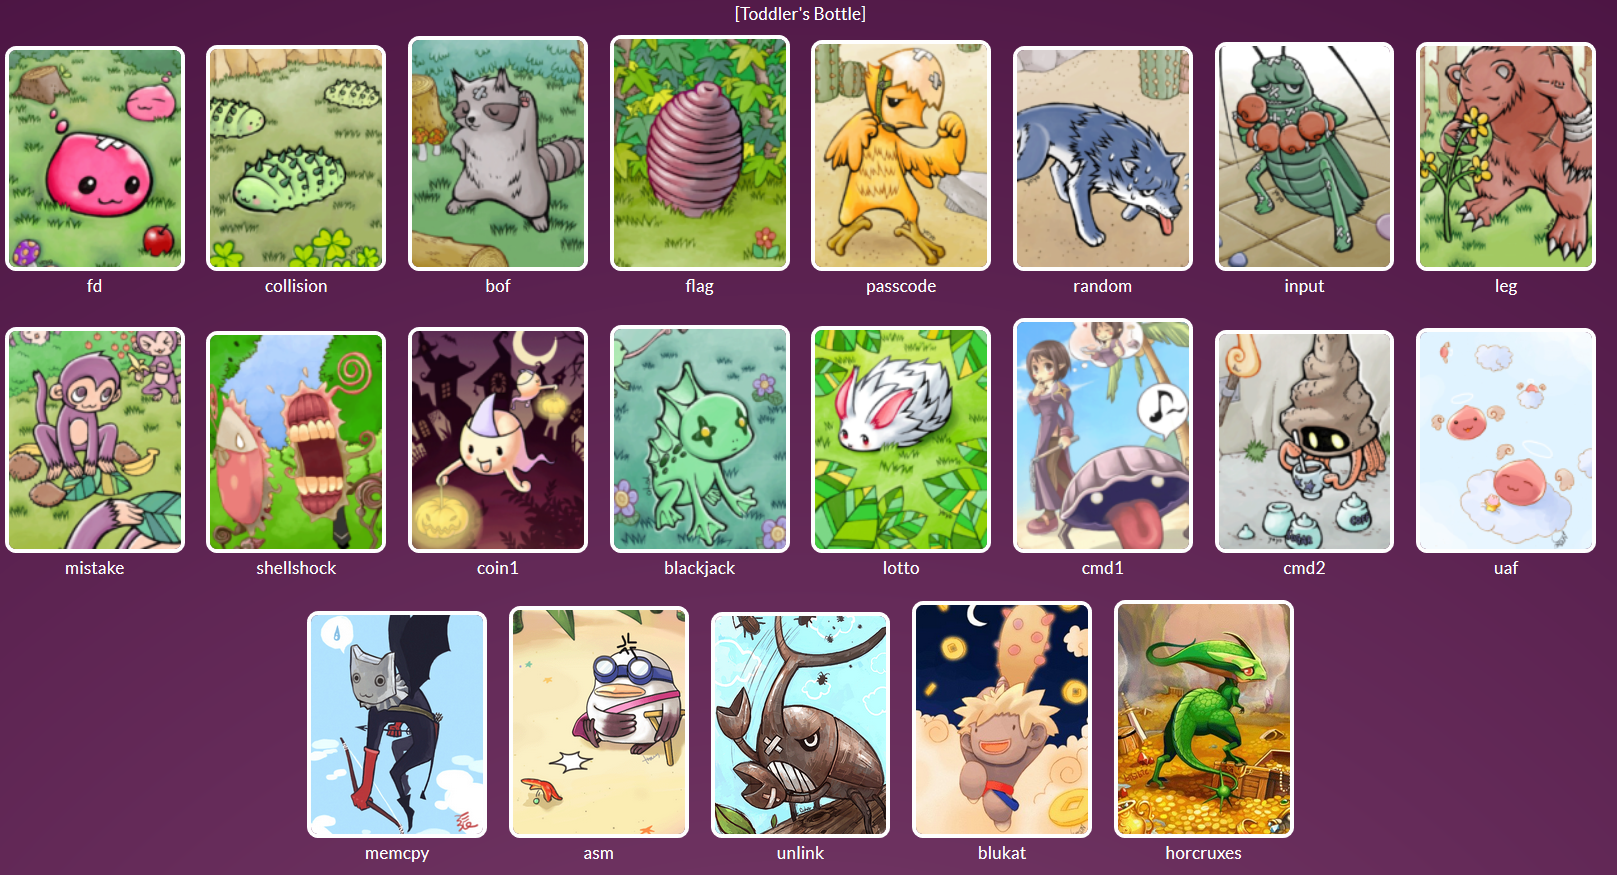
\includegraphics[max size={\textwidth}{\textheight}]{./images/all_challenges.png} 
\end{figure}

\newpage
\tableofcontents
\newpage

\parskip 1.5ex
\renewcommand{\baselinestretch}{1.33}

\section{What is this?}

\wrapimagerightcap{./images/pizza_hack.jpg}{You're not "supposed to" do that.}

It's an introduction to that part of information security that your parents warned you about.

The field doesn't have a proper name, exactly, but we know it when we see it. Systems are understood in terms of naked primitives; convenient abstractions are stripped away, or are unavailable to begin with. The narrative about \href{https://en.wikipedia.org/wiki/functional_fixedness}{how the system is "supposed to" behave} is ignored with prejudice. These systems are then understood in more detail than before, and may even be made to behave in ways that they shouldn't. Terms like "reverse engineering", "exploitation", and the by-now-kitschy "hacking" seem to figure into it. 

Unfortunately, abstractions are intuitive and legible, whereas the primitives they abstract away are neither of these things. This means that looking past abstractions is a terrible experience all around.  Still, every now and then an excited newbie hears of the above and says, "that sounds great! Where do I get started?". An embarrassed expert then answers that there is no royal road, and they should probably follow this and that person on Twitter, and "go practice, like with CTFs or something idk".

This is sound advice, but we've seen people who follow it have a bad time. There's a pervasive mentality in the field that the tao that can be taught is not the true tao, and that the only way to learn is to \href{https://www.offensive-security.com/offsec/say-try-harder/}{Try Harder\textsuperscript{\textregistered}}. As a result, exercises challenge, but don't educate. They demand would-be solvers to summon a grab-bag of disparate knowledge, to surmount minor technical gotchas that a beginner won't recognize as such, and to know how to deal with pure caprice. Solutions -- if they exist -- are provided by third parties, are unbearably terse, and are devoid of any connection to a larger picture. Most of all, they fail to answer the most pertinent question: "How was \textit{I} supposed to think of that?". The student's only recourse is to search for an easier problem and pray vigorously that, working through it, they will finally grok the general principle. It's Try Harder\textsuperscript{\textregistered} all the way down.

\wrapimageleftcap{./images/complications.png}{Barrier to entry. Also, that $\left(\frac{N}{m}\right)$ should be ${N \choose m}$.}

The upside of this is that it's realistic. Reality is not a learning opportunity; it does demand disparate information, it does frustrate with minor technical gotchas and pure caprice, and it does often leave the student no choice but to Try Harder\textsuperscript{\textregistered}. Students should be ready to deal with problems in these harsh terms, which is why we have the ageless academic tradition of final exams. Still, imagine a course comprised entirely of final exams. No theory, no guided solutions, not even proper homework problems -- just the hapless student vs. their own ignorance. People would run for the hills at such a proposal, and for good reason. No one likes being told to run before they've walked.

The buck has to stop somewhere, with a teaching moment that doesn't assume that deep down the student already knows all the answers. Georgia Tech's "Toddler's Bottle" exercises are the closest thing we've found to the missing homework problems: exercises which distil a concept, simplify its presentation, and filter out distractions. This guide, then, is an attempt to complete the puzzle: the missing guided solutions and lecture notes that walk the reader through the challenges, and try to provide context and perspective.

The buck stops here. Hopefully.

\section{What do I Need to Know Coming in?}

\wrapimagerightcap{./images/ubuntu.png}{Ubuntu Linux Desktop}

We tried to trim the list of prerequisites as much as possible and as much as time allowed. Still, some pieces of knowledge turned out to be too fundamental to route around, and too hefty to be transmitted in a digression. Throughout this document, we assume that:

\begin{itemize}
    \item You have a working \textbf{Virtual Machine} with a working \textbf{Linux Distribution}, such as \href{https://ubuntu.org}{Ubuntu Linux}, installed
    \item You know \textbf{C language} at the 101 level -- enough to know when to use \code{\&var} instead of \code{var} and how 2's complement works
    \item You know \textbf{C++ language} at the 101 level -- enough to know what polymorphism is, what inheritance is and what virtual functions are for
    \item You know enough \textbf{Python} to comfortably read it and write in it
    \item You know about \textbf{binary and hexadecimal representation}, and how to convert between those and decimal
\end{itemize}

Probably the biggest hurdle not on this list is knowing how to use a debugger and a disassembler. We tried, we \textit{really} tried, to put together a proper tutorial to bring the reader up to speed on how to use both; but these are very hefty subjects, and if you've had zero experience with a disassembler or a debugger up until now, some of the exercises may get somewhat frustrating. If mid-exercise you feel that this is the bottleneck holding you back, you probably want to put aside the problem and first complete a dedicated tutorial on these subjects.

\section{Basic Linux Commands}


In our Linux VM, let's create a new terminal (\code{ctrl+shift+t}), then try out the commands below and get a feel for how they work.

\wrapimagerightcap{./images/sandwich.png}{\href{https://xkcd.com/149/}{xkcd \#149, "sandwich"}} 

\begin{itemize}
    \item \xcode{bash}{pwd} - print the current working directory.
    \item \xcode{bash}{ls} - list files and directories in the current directory.
    \item \xcode{bash}{cd dirname} - "enter" the directory \code{dirname}, so it becomes the new current directory. To go back up in the directory structure, use the command \xcode{bash}{cd ..}. It's also possible to \xcode{bash}{cd} directly to a completely different path, e.g. \xcode{bash}{cd /tmp}; to go back to the home directory, do \xcode{bash}{cd \~}.
    \item \xcode{bash}{cat filename} - print the contents of the file \code{filename} to the terminal. 

        Can be given several files (\xcode{bash}{cat file1 file2 file3...}) and will print all of them in succession.    
    \item \xcode{bash}{cp filename1 filename2} - create a copy of \code{filename1}; the copy will have the name \code{filename2}.
    \item \xcode{bash}{mv filename1 filename2} - move the file \code{filename1} to a new location \code{filename2}.
    \item \xcode{bash}{mkdir dirname} - create a new empty directory with the name \code{dirname}. The directory will be created in the current working directory.
    \item \xcode{bash}{rm filename} - delete the file \code{filename}.
    \item \xcode{bash}{vim} - a powerful text editor which has a "write mode" and a "command mode". To start typing, press \xcode{bash}{i}; this starts write mode. To use commands (such as save, quit, etc) go back into command mode by pressing \code{esc}. Once in command mode, to save do: \xcode{bash}{:w} + return and to quit do: \xcode{bash}{:q!} + return. If \xcode{bash}{vim} is a bit too much, try \xcode{bash}{nano} instead.
    \item \xcode{bash}{chmod a+x filename} - add execution privileges to a file for everyone, so that any user can execute the file. \xcode{bash}{chmod} can also be used to add/remove read privileges (+r, -r) and write privileges (+w, -w); and can be used to modify permissions only for the file owner or file group (with u+ or g+ instead of a+). More on this below, under "access control". 
    \item \xcode{bash}{sudo} - execute a command with administrator privileges. Using this command causes the OS to prompt for the current user's account password.
    \item \xcode{bash}{groups} - print the list of groups the current user belongs to.
    \item \xcode{bash}{sudo apt install python3} - installs Python3 on the machine (chances are it's installed already, and the command will quit with a note explaining this). Other programs can be installed similarly, by specifying their name instead of \code{python3}. Since it invokes \xcode{bash}{sudo}, this command requires the current user to be admin on the machine, and will prompt for the account password. \code{apt} is the package manager for Ubuntu, Linux Mint and Debian; users of other Linux distributions (such as Arch Linux) should use whichever package manager is included with it.
    \item \xcode{bash}{python3} - starts a python shell. Try \code{2+2} and see how the shell responds. It's possible to exit the shell by typing \code{quit()}. It's also possible to do \xcode{bash}{python3 filename.py}; this will run all the commands in \code{filename.py} through the Python interpreter.
\end{itemize}

Before we're done, one neat trick that's useful to know is backtick substitution. If a bash command is placed in backticks (\xcode{bash}{`}), bash will replace it with the output it generates if itself invoked as a bash command. So, for example, in the command \xcode{bash}{cp /bin/cat `pwd`}, bash will expand \xcode{bash}{`pwd`} to the actual current directory, and create a copy of \xcode{bash}{/bin/cat} there.

\section{SSH and SCP}

It is possible to connect from a linux machine $M_1$ to another linux machine $M_2$, and run commands on $M_2$ as if sitting at the keyboard of $M_2$ in person. To do this, one must know $M_2$'s IP address, know which port its SSH server is running on, and have valid credentials for an $M_2$ user account.

This is done by going to $M_1$ and executing: \xcode{bash}{ssh user@1.2.3.4 -p 1001} where \code{1.2.3.4} should be $M_2$'s IP address, \code{1001} the SSH port and \code{user} the username at $M_2$. The remote machine will issue a password prompt for \code{user}. If verification is successful, an SSH session is established and the user at $M_1$ can now issue commands remotely to $M_2$. To stop issuing commands to $M_2$ and go back to the $M_1$ command line, one should use the command \xcode{bash}{exit}.

Apart from starting an SSH session, it is also possible to copy files from $M_1$ to $M_2$ and back, by using $M_1$'s command line. This is done using the \xcode{bash}{scp} command. To copy the file \code{/home/bob/grocery\_list.txt} from $M_2$ to $M_1$, execute the command \xcode{bash}{scp -P 1001 1.2.3.4:/home/bob/grocery\_list.txt ./grocery\_list.txt}. To copy the file back to the remote $M_2$, execute: \xcode{bash}{scp -P 1001 ./grocery\_list.txt 1.2.3.4:/home/bob/grocery\_list.txt}.

\wrapimageleft{./images/ssh.png}
The server at \code{pwnable.kr} runs an SSH server in port 2222; one of the accounts on that machine has username \code{fd} and password \code{guest}. Try to establish an SSH session using that server and that account:

\xcode{bash}{ssh fd@pwnable.kr -p 2222}

When prompted for a password, write "guest" and hit return (the password will not appear on screen).  Verify that the SSH session has been successfully established. Create a directory under \code{/tmp/}:

\xcode{bash}{mkdir /tmp/an\_original\_dir\_name}

(use something original instead of \code{an\_original\_dir\_name}; the command will fail if someone else has already created a directory by that name)

Exit the session with \xcode{bash}{exit}.

Now, try to copy the file \code{/home/fd/fd.c} from the remote server to the current directory:

\xcode{bash}{scp -P 2222 fd@pwnable.kr:/home/fd/fd.c .}

Another password prompt will appear (it's still \code{guest}). Verify that a copy of \code{fd.c} is now present on the local machine.

Try to send a file back to the pwnable server. 
\begin{lstlisting}[language=bash]
echo "testing" > test.txt
scp -P 2222 ./test.txt fd@pwnable.kdr:/tmp/an_original_dir_name/test.txt
\end{lstlisting}

Start another SSH session and verify that a copy of \code{test.txt} is really there.

We wish we could just breezily explain how to troubleshoot network issues, \textit{just in case} there are any. Alas, if we started, we'd get to the actual material on page 50 or so. If an SSH connection fails and you've never resolved a similar issue on your own before, go ask someone for help. 

\section{Access Control}

Nearly every challenge on pwnable.kr is of the form: "here's a program; get clever with it and make it access the flag". If you honestly don't care why you can't just read the flag directly on your own, and you're willing to deal with plenty of trial and error when trying to read/create files and directories, then in theory you can go ahead and skip this section. In practice, we suggest you don't.

\subsection{File Permissions}

\wrapimageright{./images/file_permissions.png}
As we've mentioned above, the concept of \textit{boundaries} is deeply interwoven into digital system best practices. By default, Alice should not have access to documents created by Bob. By default, if Bob visits a website the website should not have the ability to meddle with Bob's \code{My Documents} folder, and his web browser should not have the ability to install another operating system on his machine. In its most idealized form, this is called the \textbf{Principle of Least Privilege} (PLP): entities should have exactly the privileges necessary to carry out their duties, and no more.

We live in the real, non-idealized world, where violations of the PLP are a fact of life. Still, most digital systems do have a form of access control -- a system for determining who has the right to do what. In the real world, entities do not always have the least possible privilege, but they are typically subject to just enough limitations to prevent anything outright insane.

Linux, in particular, has a certain system in place that limits access to files. This may not sound like much, except in Linux everything is a file, so it's really more accurate to say that this system limits access to everything.

To see this system in action, on the Linux machine, execute the following mysterious commands. Each invocation of \xcode{bash}{sudo} might require your admin account password, which you picked when you installed the OS.
\begin{lstlisting}[language=bash]
cd ~
mkdir ac_test
cd ac_test

sudo groupadd characters

sudo useradd alice
sudo usermod -a -G characters alice
sudo passwd alice
#when prompted for password
drinkme
#when prompted again
drinkme

sudo useradd bob
sudo usermod -a -G characters bob
sudo passwd bob
#when prompted for password
fixit
#when prompted again
fixit

touch jabberwocky.txt

echo "twas brillig etc" > jabberwocky.txt
sudo chown alice jabberwocky.txt
sudo chgrp characters jabberwocky.txt

touch collab_diary.txt
echo "today was a great day" > collab_diary.txt
sudo chown alice collab_diary.txt
sudo chgrp characters collab_diary.txt
sudo chmod g+w collab_diary.txt

touch yes_we_can.txt
sudo chown bob yes_we_can.txt
sudo chgrp characters yes_we_can.txt
sudo chmod og+w yes_we_can.txt
\end{lstlisting}

When done, execute \xcode{bash}{ls -l}. The output should look like this: 

\displayimage{./images/access_control_file_list.png}

\wrapimageright{./images/file_permissions_how_to_read.png}
There's some amount of information here to unpack. First, we got quite a lot more output than with a simple \xcode{bash}{ls}; this is because we specified the \xcode{bash}{-l} flag, which causes \xcode{bash}{ls} to output additional information. This additional information includes each file's access permissions, which we are interested in.

The access permissions for each file are the very first blob of characters on the line that ends with the file name. So, in the example above, \code{collab\_diary.txt} has access permissions \xcode{bash}{-rw-rw-r--}.

Here's how to read these permissions:
(Ignore the first - for the time being.)
\begin{itemize}
    \item The \textbf{owner} of the file can...
    \item \xcode{bash}{r}ead it
    \item \xcode{bash}{w}rite to it
    \item \xcode{bash}{-} but not execute it
    \item The \textbf{group} associated with the file can...
    \item \xcode{bash}{r}ead it
    \item \xcode{bash}{w}rite to it
    \item \xcode{bash}{-} but not execute it
    \item Anyone \textbf{else} can...
    \item \xcode{bash}{r}ead the file
    \item \xcode{bash}{-} but not write to it
    \item \xcode{bash}{-} or execute it
\end{itemize}

The access permissions are followed by the mysterious number 1 (leave that alone for the time being, too). Following \textit{that}, one can see the user who owns the file and the group associated with the file.

For instance, in the example above:
\begin{itemize}
    \item Alice, and any member of "characters", can read \code{collab\_diary.txt} and write to it. Anyone else can only read the diary, but not write to it.
    \item Alice can read \code{jabberwocky.txt} and write to it; anyone else can only read it, whether they are a member of "characters" or not.
    \item Anyone can read \code{yes\_we\_can.txt} or write to it.
\end{itemize}

Feel free to experiment with the various files and permissions. It's possible to switch users with the \xcode{bash}{su} command - for example, \xcode{bash}{su alice} (this will provoke a prompt for Alice's password; this is \code{drinkme}. Bob's password is similarly \code{fixit}). To resume using the main user account, use the command \xcode{bash}{exit}. Try to read and modify the various files while acting as that account, then as Alice and as Bob, and see whether the results match your expectations. Note that we've made both Alice and Bob members of the "characters" group.

Just as files have read, write and execute permissions, so do directories. A user having "read" permission for a directory means they are allowed to see its contents; "write" permission means they are allowed to create and remove files from it; and "execute" permission means they are allowed to \xcode{bash}{cd} into it.

\subsection{SUID bit}

\wrapimageright{./images/baton.png}
Here's a trick question. Suppose Alice \textit{executes} a file owned by Bob; which permissions should the program have -- Alice's or Bob's?

If we answer "Alice's" then we have a problem. Suppose the file was the command \xcode{bash}{passwd}; in this case, Alice is trying to change her account password, and Bob is the system administrator. Now \xcode{bash}{passwd} will run with Alice's permissions. But all account passwords are stored in the same file. Alice can't read it, or write to it (if she can, that's a serious security breach). Therefore, if \xcode{bash}{passwd} is run with Alice's privileges, it can't do its job of changing Alice's password.

But if we answer "Bob's", then we \textit{also} have a problem. Suppose that Bob has created a simple text editor. He owns the file for the text editor executable. If Alice tries to use the text editor, she'll find that instead of her own files, she can only edit Bob's files! This is not good news for either Alice's productivity of Bob's privacy. 

Because of the above issues, the answer is not "Alice" or "Bob"; the answer is "Bob should get to decide, on a per-file basis". This is implemented via a feature called "suid". Executable files will, by default, run with the permissions of whoever executed them. But if suid is on for that file, and it is a \textbf{binary} file, then it will run with the permissions of the file owner. We therefore expect that \xcode{bash}{passwd} should have suid on, and in fact, it does:

\displayimage{./images/suid_passwd.png}


The \xcode{bash}{s} (instead of \xcode{bash}{x}) in the permissions for the file owner indicates that suid is on for this file. 

suid can be turned on or off for a file using \xcode{bash}{chmod} -- with \xcode{bash}{u+s} or \xcode{bash}{u-s} respectively. Again, this only applies to binary files - not scripts!

Let's test out the way SUID works. Execute the following commands:

\begin{lstlisting}[language=bash]
cd ~/ac_test
echo "Alice's secret" > ./alice_secret.txt
sudo chown alice ./alice_secret.txt
sudo chgrp characters ./alice_secret.txt
sudo chmod og-rwx ./alice_secret.txt

cp /bin/cat .
sudo chown alice ./cat
sudo chgrp characters ./cat
sudo chmod a+x ./cat

cp /bin/cat ./cat_suid
sudo chown alice ./cat_suid
sudo chgrp characters ./cat_suid
sudo chmod a+x ./cat_suid
sudo chmod u+s ./cat_suid
ls -l
\end{lstlisting}

The output should look something like the below: 

\displayimage{./images/alice_bob_suid.png}

Take a moment to guess the output of the following commands:

\begin{lstlisting}[language=bash]
su bob
fixit #when prompted for password
./cat alice_secret.txt
./cat_suid alice_secret.txt
\end{lstlisting}

The call using \xcode{bash}{cat} fails, because it runs with Bob's permissions and he does not have read permissions for \code{alice\_secret.txt}. The call with \code{cat\_suid} succeeds, because due to suid being on, it runs with Alice's permissions.

\section{Linux File Descriptors}

A lot of things in Linux are files. Directories are files. Hard disks are files. Processes are files. Internet connections are files. \textit{Files are files}.

\wrapimageright{./images/file_descriptors.png}
We've seen how to work with files on Linux: creating files, modifying the contents of files, copying and moving files. It's a pretty intuitive API, so of course it's the result of an abstraction on top of an abstraction on top of thirty other abstractions. Let's ask the question bluntly: The command line shell we are using, \code{bash}, was written in C language -- so how did its author create \code{bash} without already having \code{bash} to handle all the file operations?

The answer is that C (and assembly) programs use a filesystem API which is a layer of abstraction down from \code{bash}. Consider the following C program: 

\lstinputlisting[language=C]{./code/fd_demo.c}

Every process in Linux (and Windows, too) has a number which is its process id (pid). This number uniquely identifies the process. The above program, when launched, will display the pid of its own process. Launch the program, then on a different terminal execute the following command: \xcode{bash}{ls -la /proc/<pid>/fd} where \code{<pid>} should be replaced with the actual pid that the process reported. The output should look something like this:

\displayimage{./exercises/00_fd/fd_before_open.png}

On the original program terminal, press return. Now on the other terminal run \xcode{bash}{ls -la /proc/<pid>/fd} again.  The specific details will vary, but there should be something in the ouptut that wasn't there before:

\displayimage{./exercises/00_fd/fd_after_open.png}

The reader might wonder what file descriptors 0, 1 and 2 are; these are the process' \textit{standard input}, \textit{standard output} and \textit{standard error} streams, respectively. These three file descriptor numbers are always the same for every process (so, for example, the standard input is always descriptor number 0). The standard output is where program output is written, and the standard input is where input is taken from. Right now, both are bound to the same value: \code{/dev/pts/7}, which is the terminal that launched the C program (your value will probably be different). Let's do an experiment:

\xcode{bash}{echo "hi" > /dev/pts/7}

Go look at the terminal that spawned the C program; the word \code{hi} should appear there. 

\section{Challenge 0x00: fd}

\exerciseopen{./images/00_fd.png}{Mommy! What is a file descriptor in Linux?}

Visit pwnable.kr, create an account and click "play" at the top menu. Choose the first challenge in the "toddler's bottle" category -- \code{fd}. We're given the IP address, port and credentials for an SSH session.


After establishing an SSH session with the correct parameters, the following message should appear:

\displayimage{./exercises/00_fd/fd_welcome_message.png}

Following the logon, the session sets the current directory to the home folder of the remote user whose credentials were used (in this case, the user is \code{fd} and so the current directory is set initially to \code{/home/fd}). Let's look at the files in that directory and their permissions:

\displayimage{./exercises/00_fd/fd_permissions.png}

Since we're playing Capture The Flag, we turn our interest to the file labeled "flag". Unfortunately, based on its permissions, owner and group, to read it we need to be logged in as \code{fd\_pwn} or belong to the \code{root} group.

Or maybe there's another option? We have execute permissions for the file \code{fd}, which belongs to the user \code{fd\_pwn} \textit{and} has suid turned on. In other words, if we run \code{fd} and convince it to read and output the flag for us, we win. This is a pretty standard setup for CTF exercises; the whole challenge revolves around cajoling \code{fd} to do our bidding in some way -- which may be easy, difficult, head-against-the-wall difficult, or even impossible (though in that last case, it's less of a proper exercise and more of an exercise in futility).

How do we get \code{fd} to print the contents of "flag" for us, then? Conveniently, we have been given the source code for the \code{fd} program in the file \code{fd.c}:

\lstinputlisting[language=C]{./exercises/00_fd/fd.c}

The program takes the first parameter as a number, subtracts \code{0x1234} from it and reads 32 bytes from the file descriptor with that number. If the result is \code{LETMEWIN}, the program prints the flag.

When CTFing (and solving problems in general), a precise concept of what we \textit{can't} do and what we \textit{don't} know can be a valuable asset. For example, when the \code{fd} program runs on the remote server, we can't:

\begin{enumerate}
    \item access \code{fd}'s list of open file descriptors; we don't have read access to \code{/proc/}
    \item directly interfere with the list of open file descriptors; we don't have write access to \code{/proc/}, either
    \item modify our choice of \code{argv[1]} retroactively after the program has been run
    \item get the \code{fd} process to open a file for us, thus adding an entry to its file descriptor table; the program source code mandates no such action 
\end{enumerate}

Problems 1 and 3, in themselves, are solvable -- somewhat. We've seen that when a process opens a new file, that file is assigned the next available free file descriptor. Therefore, typically the first file opened has descriptor 3, the next one 4, and so on. This implies that if the program source had contained an extra line: 

\begin{lstlisting}[language=C]
fd = open("read_from_here.txt",O_RDONLY);
\end{lstlisting}

We could guess that \code{read\_from\_here.txt} would be assigned a file descriptor of 3. We could then solve the challenge the following way: create the file \code{read\_from\_here.txt} in advance with the contents \code{LETMEWIN}, and then execute \code{fd 4663}; 4663 is chosen because \xcode{bash}{4663 = 0x1234 + 3}. The program \code{fd} would compute \xcode{bash}4663-0x1234 = 3\xcode{bash}, read 32 bytes from the file associated with file descriptor 3 (that's \code{read\_from\_here.txt}), see that it is the correct value \code{LETMEWIN} and print the flag.

There are two problems with the above solution draft. First, we will run into permission issues when trying to write to \code{read\_from\_here.txt}; we don't have write permissions for the \code{/home/fd/} directory on the remote server. Second of all and more importantly, this is all a hypothetical situation. In the actual program, there is no \code{read\_from\_here.txt}. Our idle dream bubble goes poof, and we must face the problem in its original, actual form.

What \textit{do} we know for sure about the state of the \code{fd} process' file descriptor list, then? Not much. All we know for sure is that the 3 first descriptors (0, 1 and 2), representing the standard input, output and error, will all be bound to the \code{/dev/pts} terminal that spawned the program. We are effectively forced to choose an \code{argv[1]} value of \code{0x1234+0}, \code{0x1234+1} or \code{0x1234+2}; any other value will be a futile shot in the dark. We've seen that by default, processes don't \textit{have} open file descriptors other than these three.

Translated into English, this means we can tell the program to read the 32 bytes either from the standard input, the standard output, or the standard error stream. And, once we've said that out loud, that first option should sound pretty attractive to us. "Reading from the standard input" is a very common C idiom; it's what happens, for example, when a C program calls \code{getchar()} or \code{scanf()}. If we can get the program to "read 32 bytes from the standard input", what this means in practice is that the program will halt and wait for us to input those 32 bytes manually from the terminal!

This insight yields the solution; simply run \code{fd 4660} (since \code{4660 = 0x1234}). Instead of chastising us to learn about file IO, the program will seem to halt and wait for our input. Write \code{LETMEWIN}, press return and the program will print the flag.

Generally speaking, when a CTF challenge is doing something strange and apparently meaningless with its given input, it \textit{may} be the case that the answer is just \textit{very simple} and the author didn't want anyone to stumble upon it blindly. Without the artificial factor of \code{0x1234} introduced here, it's very feasible to imagine people just trying to run \xcode{bash}{fd 0} to see what happens. 

In this sort of situation, if we're looking to get the flag and do zero learning, we can try to send input that \textit{after} the meaningless transformation becomes exactly the sort of thing that someone might mindlessly type. It's a shot in the dark, but it's very worth it if and when it pays off (it works for one of the later exercises in the sequence, so stay tuned).

\section{Hexadecimal Representation, Special Characters and the xxd program}
There are 256 possible bytes, all of which we may need to provide to various programs as input, and fewer than half of which appear on our keyboard. This is a problem.

One way of getting around the problem is inserting special characters into the terminal by pressing \code{ctrl+shift+u}, followed by the desired unicode hex value, and then return (try this in the terminal right now with the value \code{41}, and verify that this inserts an \code{A} into the command line). But we don't generally recommend this approach. First of all, most of the time, we'll need values to be ascii-encoded and not 2-byte unicode values. Second, imagine inputting a sequence of 300 special characters into the terminal with this method, again and again, in order to debug an issue with how a program reacts to the input! It's a sure way to go insane.

The reader might ask, "can't I just construct the input with a script and send it to the process via, I don't know, some Python module or another?". That's an excellent question; this "some module or another" is called \code{pexpect}, and yes, it would solve the immediate problem. But considering where we are right now in the challenge sequence, \code{pexpect} is overkill. It's bad form to reach for complex tools when dealing with simple problems.

Instead, we're going to tackle the issue with backtick substitution (we already saw that trick under "basic linux commands"), a bash feature called \textit{IO redirection} and a tool called \code{xxd}.

\code{xxd} converts input from raw bytes to hexadecimal representation. The easiest way to understand how it works is to see an example. Create a new file, named \code{xxd\_demo}, with the following contents:

\lstinputlisting{./code/xxd_demo}

Now run:

\xcode{bash}{xxd xxd\_demo > xxd\_demo.hex}

This should create a new file with the name \code{xxd\_demo.hex}. Open it in a text editor:

\lstinputlisting{./code/xxd_demo.hex}

Now run:

\xcode{bash}{xxd -r xxd\_demo.hex > xxd\_demo\_2}

Open \code{xxd\_demo\_2}. It should be identical to \code{xxd\_demo}. As we've just demonstrated, \xcode{bash}{xxd -r} converts from hexadecimal representation back to raw bytes. 

One thing that's important to note is that in the hexadecimal representation used by \code{xxd}, the first number in each line corresponds to the offset in the file, and each line specifies at most 16 bytes. So we can't, for example, just write \code{41} 80 times, and have \xcode{bash}{xxd -r} convert it into 80 "A"s. To see how we \textit{do} get 80 "A"s, simply create a file containing 80 "A"s and run \xcode{bash}{xxd} on it.

\wrapimageleft{./images/ascii_table.png}
\code{xxd} is not the only way to feed special characters to linux programs. For small use cases, one can also use \code{printf}, which is a shell built-in rather than a program (this means we can still use it if we accidentally wipe \code{/usr/bin}; this is actually relevant later in one of the exercises). Try \xcode{bash}{printf "\\x41\\x42\\x43\\x44"}. If one must specify characters directly from the terminal and does not have access to \code{xxd} or \code{printf}, they can also use character substitution with the \code{\$} sigil. Try: \xcode{bash}{echo \$'\\x68\\x65\\x6c\\x6c\\x6f'}; this should echo \xcode{bash}{hello} to the terminal. Both these methods can be similarly used to specify special characters directly from the terminal to other programs. The \code{\$} sigil can also be used to an effect similar to backtick substitution; try \xcode{bash}{\$(echo ls)}.

As for IO redirection -- it is a fanciful name for a really simple feature. We can have a program read from a file instead of the terminal, or write to a file instead of the terminal, or both. To have a program write to a file instead of the standard output, do \xcode{bash}{program > file}; to have it read from a file instead of the standard input, do \xcode{bash}{program < file}. To do both: \xcode{bash}{program < in\_file > out\_file}. Actually, a lot of commands we've typed so far involve IO redirection.

An important caveat is that when redirecting stdin, once the input file is exhausted, it is not possible to interact any further with the target process. The program will simply assume there is no more input, and react accordingly.

How do \code{xxd}, IO redirection and backtick substitution solve our problem? Well, if we want to feed a program a certain complicated input full of strange characters, we can first create a file (let's name it \code{input.hex}) that contains the input in hexadecimal representation. Then run \xcode{bash}{xxd -r input.hex > input.dat} to get our input in raw bytes form sitting in the file \code{input.dat}; then, finally, to feed the input to the program, execute \xcode{bash}{program < input.dat}.  To redirect to or from the standard error channel, we can use \code{2>} or \code{2<} (this is esoteric and not used very often, but it crops up in one of the exercises). If instead we want to give our input as a command line argument, we can use backtick substitution: \xcode{bash}{program `cat input.dat`}.

Are we done? Almost. Even now, some gotchas remain that we should be aware of. Not all bytes were created equal, and some bytes may cause our specially crafted input to not carry over into the program. In particular, command line parameters typically don't play well with the null byte (\code{0x00}), the tab (\code{0x09}), the newline (\code{0x0A}) and the space character (\code{0x20}). Methods that read from the standard input are even more picky, and apart from the bytes already mentioned, might also have trouble with the end-of-transmission byte (\code{0x04}), the vertical tab (\code{0x0B}), the form feed (\code{0x0C}) and the carriage return (\code{0x0D}). If a targeted program is acting up because of problematic bytes, try to think of an alternative input which does not contain these bytes, but achieves the same goals.

\section{Hash Functions}

A \textbf{hash function} is a function $h$ that fulfils two conditions. 

First, it maps input of arbitrary length to output of a fixed length of $n$ bits. For example, the hash function \code{sha256} can take any input, and will produce an output which is 256 bit long. 

\wrapimageright{./images/hash_functions.jpg}
Second, for $h$ to be considered a \textit{really} proper hash function, $h$'s output needs to have been produced by a certified ancient deity at the dawn of time. The deity must have gone over every possible input out of infinitely many, and assigned each input a single $n$-bit output, perfectly at random out of all possible strings of $n$ bits. Once this ritual is complete, $h$ is ready for use. Every time $h$ is computed for some input $x$, the deity must be consulted directly for the correct value of $h(x)$.


If this story sounds somewhat suspicious to you, we'll further say that all the hash functions you've heard about, like \code{sha1} and \code{md5}, are actually knock-offs created by mortals. These are mere human-written functions, cleverly designed to create output "random enough" to seem like the real deal. Some of the knockoffs are pretty good; \code{sha256} can be treated, for all practical purposes, as if it were the real thing. \code{sha1} and \code{md5} are okay-ish, but best avoided. Most importantly of all, if we try and write our own hash function from scratch right now, it will end badly.


\wrapimageleftcap{./images/hash_function_creation.jpg}{the original, perfect hash function being bestowed unto man. It has since been lost.}

How so? Hash functions are useful, for example, for dealing with account passwords. We can pick a hash function $h$ and then, instead of storing Alice's password $p$ on a server, we can store $h(p)$. Every time Alice logs in, she provides a password $p'$ and we verify that $h(p')=h(p)$ to approve the login. Now if the database leaks, instead of $p$ an attacker only has $h(p)$. If the hash function is really proper, it's not clear how an attacker can proceed from there. They can try asking the relevant deity to "un-compute" the hash and recover $p$, but the deity will certainly refuse to answer and probably smite them for their insolence.

But what if we're using our own weak knock-off hash function? Well, it might be weak enough that it's actually possible to recover $p$ back from $h(p)$. This renders the "hash passwords" protection completely useless. Because of this, if one can efficiently find \textit{preimages} for $h$ -- that is, given $h(p)$ easily find a $p'$ with $h(p')=h(p)$ -- then $h$ is officially declared a lousy knockoff, and unfit for use.

(As an aside, a hash function knockoff $h$ is also considered lousy if one can efficiently find \textit{collisions} for it: that is, pairs $p_1, p_2$ where $p_1 \neq p_2$ but $h(p_1)=h(p_2)$. But we'd rather not get into that right now.)

Just to get a feel of how hash functions operate, execute \xcode{bash}{python3} and inside the python shell do:

\lstinputlisting[language=python]{./code/hash_demo.py}

This should output:

\lstinputlisting{./code/hash_demo.out}

Which is the \code{sha256} value of \code{hello world} in hexadecimal notation.

A rule of thumb is that if a hash function is at least okay-ishly proper then its implementation will be complex, full of redundancy, complicated, ugly and full of redundancy. It'll be called from some third-party library and have its own Wikipedia entry. If a function is purporting to be a hash function but it's simple, elegant, and seems like it was invented on the spot by someone who's never heard of this whole deity business -- it might be possible for an attacker to find preimages and wreak all kinds of mischief. 

\section{Challenge 0x01: collision}

\exerciseopen{./images/01_collision}{Daddy told me about cool MD5 hash collision today. I want to do something like that too!}

This exercise should really be called "preimage", but we understand how that's less catchy.

As usual, we're given the IP address, port and credentials for an SSH session. We are again provided with a program \code{col} which has permission to read \code{flag}, and will print it for us if we give it the correct input. Also similarly to the previous challenge, the remote folder has \code{col}'s source code, \code{col.c}:

\lstinputlisting[language=C]{./exercises/01_collision/col.c}

The function \code{check\_password} is something akin to a hash function: it takes input and generates a 4-byte output. We say "something akin" for two reasons:
\begin{enumerate}
    \item \code{check\_password} only takes an input length of exactly 20 bytes. A proper hash functions can take input of arbitrary length. 
    \item more importantly, it's a simple and elegant function with no Wikipedia entry. Therefore, as we've learned, it's broken.
\end{enumerate}

The challenges requires that we find a preimage for \code{check\_password}, which is exactly the sort of thing an attacker can do when a hash function is broken. We're given the value \xcode{C}{hashcode = 0x21DD09EC} and need to provide a password such that \xcode{C}{check_output(password) == hashcode}.

Looking at \code{check\_password}, we quickly conclude that it simply computes the 2's complement sum of the 5 dwords in the 20-byte password (with each dword interpreted as a little-endian integer). Since 2's complement is equivalent to addition modulo $2^{32}$, we simply need to find 5 integers that sum to \code{0x21DD09EC}. 

Or do we? Consider that one such solution is \code{0x21DD09EC, 0, 0, 0, 0}; but if we try that, all the \code{0} values will be encoded as strings of null bytes. As we've seen above, in "special character woes", if we try to give the program such an input, it will simply assume that the input terminated on the first null byte. So, to be more precise, we need to find 5 integers which sum to \code{0x21DD09EC} modulo $2^{32}$ -- and, in their hexadecimal representation, don't contain any problematic special characters that don't play well with \code{argv} (\code{00}, \code{09}, \code{0A} and \code{20}).

Even with this limitation, the number of possible solutions is staggering; ironically, there are so many possible solutions that one might have difficulty pinning down a concrete way forward. One insight that can mitigate this issue is that for any four numbers $a, b, c, d$, there is exactly one $e$ that will result in the correct sum (\code{e = 0x21DD09EC - (a+b+c+d)} modulo $2^{32}$). So, one possible approach is to randomly pick some values of $a, b, c, d$ that lack any special characters, and hope that we get an $e$ that contains no special characters, either. If we fail, we can just try again with different values for $a, b, c, d$.

Let's try something banal: $a = b = c = d =$\code{0x41414141}. We then use Python to compute:

\xcode{python}{e = (0x21DD09EC - 4*0x41414141) \% 2**32}

This returns the number \code{483919080}, or \code{0x1cd804e8} in hexadecimal (we can ask Python to compute this for us by issuing the command \xcode{python}{hex(e)}). We got lucky on our first try: the resulting value of $e$ does not contain any problematic bytes. We now compose our crafted password in hexadecimal: 

\lstinputlisting{./exercises/01_collision/pass.hex}

And issue the command:
\xcode{bash}{xxd -r pass.hex > pass}

This writes the password to the file \code{pass}. Run \code{col} with the contents of \code{pass} as the first parameter:

\xcode{bash}{./col `cat pass`}

And this should get the program to display the flag. Now, take a deep breath. The next exercise is somewhat of a milestone, and we're in for a journey before we get there.

\section{Computation at the Machine Level}

\subsection{Machine Code \& Assembly Language}

\wrapimageright{./images/simple_assembly.png}
We can write a program in C, but when we run the program, our machine doesn't actually \textit{run} the C. The part of our machine responsible for running programs only understands machine code. 
There are many different machine codes out there, and our machine only understands one. For instance, a standard laptop likely understands "x86" machine code, and the average cell phone likely understands "ARM" machine code. When we compile a C program, what actually happens is that our compiler converts the program into machine code (plus a bunch of metadata to help our machine run it). The machine code implements the functionality we specified in our C source.

At this point the reader might protest, "why do we need both C and machine code, then? This is confusing". That's a good question with a complicated answer. The short of it is that humans are decent at reading and writing C, but less adept at reading and writing machine code; whereas machines can be easily designed to read, write and execute machine code -- but are much more difficult to design to directly read, write or execute C.

Historically, machine code came first. For a while, humans programmed by directly writing machine code, and they were miserable. C language, and its compiler, were invented in the 1970s to alleviate this pain somewhat.

Let's take a look at some assembly language. Download the \href{https://www.hex-rays.com/products/ida/support/download_freeware.shtml}{free version of IDA pro disassembler 7.0} and install it on a Windows machine. Copy the below C code to a file named \code{hello\_assembly.c}. Compile it with:

\xcode{bash}{gcc -m32 -o hello_assembly hello_assembly.c} 

Copy the resulting program to the windows machine.

\lstinputlisting[language=C]{./code/hello_assembly.c}

Open the \code{hello\_assembly} program in IDA pro. After some grinding and churning, it should display something like the below:

\displayimage{./images/hello_assembly_x86.png}

This is x86 machine code. (Well, fine; machine code is actually ones and zeros -- this is x86 assembly language, which is equivalent but marginally more human-readable. It's possible to see the machine code by choosing \code{options->general} and changing \code{number of opcode bytes} to 10; we recommend it.)

Most people remember the first day they see, with their own eyes, that a humble "hello world" program is secretly this bunch of insufferable nonsense -- a pile of \asm{push}es and \asm{mov}s and \asm{lea}s and what-have-you. We inflicted this trauma on you for good reason; it's a necessary rite of passage.

How does a machine (such as a laptop) run the machine code? Let's say it picks the first instruction after the label \asm{main} (in the picture, that's \asm{lea ecx, [esp+4]}) and starts executing the instructions, one by one. If it runs out of instructions, it screams and dies painfully. This is not exactly true, but close enough to the truth for our purposes. So, when this program is run, first \asm{lea ecx, [esp+4]} is executed; then \asm{and esp, 0xFFFFFFF0}; then \asm{push dword ptr [ecx-4]}; and so forth.

\wrapimageleft{./images/process_memory.jpg}
Every byte in the memory space has an \textit{address}. This includes all the data, all the code for execution, the stack and heap (which we'll learn about later) - everything. It's possible to see address numbers in the IDA disassembler by pressing space; to go back to graph view, press space again.

x86 machine code can run on our laptop because the laptop has an x86-compatible processor. This processor contains a bunch of \textit{registers} - memory stores, each 4 bytes long; and supports a bunch of \textit{instructions}. We've already seen the instructions; these are the \asm{push}es, \asm{mov}s and \asm{lea}s. They typically manipulate the content of registers, or manipulate the control flow so that the next instruction that gets executed is some other instruction, instead of the next one directly below.

To have a passable knowledge of x86 architecture, one should at least know a shortlist of registers and what they are for, as well as a shortlist of instructions and what they are for. We dutifully include both. Don't get too worked up over all the references to the "stack" -- pushing into it, popping into it, its top and bottom and so on. We'll get into that in a short moment. Right now, it's enough to know that the "stack" is some region of memory, and that it used for handling function calls and local function variables. The more important thing is to become familiar with these registers and instructions.

\begin{figure}[H]
\centering
\begin{tabular}{|c|c|c|}
    \hline
    \textbf{register} & \textbf{what it's for} & \textbf{often seen} \\
    \hline 
    \asm{eax} & general purpose & carrying function return values \\
    \hline 
    \asm{ebx} & general purpose & storing values when \asm{eax} is already taken \\
    \hline 
    \asm{ecx} & general purpose & doing the counting for a \xcode{C}{for} loop \\
    \hline 
    \asm{edx} & general purpose & joining with \asm{eax} to store 64-bit numbers \\
    \hline 
    \asm{esi} & general purpose & holding an address to copy bytes from \\
    \hline 
    \asm{edi} & general purpose & holding an address to copy bytes to \\
    \hline 
    \asm{esp} & stack pointer & holding the address of the stack frame top \\
    \hline 
    \asm{ebp} & frame pointer & holding the address of the stack frame bottom \\
    \hline 
    \asm{eip} & instruction pointer & holding the address of the current instruction \\
    \hline 
    \asm{flags} & flags & keeping results of comparisons \\
    \hline 
\end{tabular}
    \caption{Table of choice x86 registers}
\end{figure}

\begin{figure}[H]
\centering
    \begin{tabular}{|c|c|c|p{0.5\textwidth}|}
    \hline
    \textbf{instruction} & \textbf{english} & \textbf{example} & \textbf{english} \\
    \hline 
    
        \asm{mov} & move & \asm{mov eax, ebx} & copy the value in \asm{ebx} into \asm{eax} \\
    \hline 
    
    \asm{inc} & increment & \asm{inc ecx} & increase the value of \asm{ecx} by 1 \\
    \hline 
    
    \asm{dec} & decrement & \asm{dec ecx} & decrease the value of \asm{ecx} by 1 \\
    \hline 

    \asm{cmp} & compare & \asm{cmp eax, ecx} & compare \asm{eax} with \asm{ecx} and remember which is larger \\
    \hline 

    \asm{add} & add & \asm{add eax, ecx} & add the values of \asm{eax} and \asm{ecx} then put the result in \asm{eax} \\
    \hline 

    \asm{sub} & subtract & \asm{sub eax, ecx} & subtract the value of \asm{ecx} from that of \asm{eax}, and then put the result in \asm{eax} \\
    \hline 
    
    \asm{mul} & multiply & \asm{mul ebx} & multiply the value of \asm{eax} by the value of \asm{ebx}, and then put the 64-bit result in \asm{edx} (significant 32 bits) and \asm{eax} (remaining 32 bits)\\
    \hline 

    \asm{div} & divide & \asm{div ebx} & treat \asm{edx} as 32 significant bits, \asm{eax} as 32 remaining bits; divide result by the value of \asm{ebx}; put the quotient in \asm{eax} and the remainder in \asm{edx} (phew!) \\
    \hline 
    
    \asm{and} & and & \asm{and eax, edx} & compute the bitwise and of \asm{eax} and \asm{ecx}; put the result in \asm{eax} \\
    \hline 

    \asm{xor} & exclusive or & \asm{xor eax, ecx} & compute the bitwise exclusive-or of \asm{eax} and \asm{ecx}; put the result in \asm{eax} \\
    \hline 

        \asm{lea} & load effective address & \asm{lea edx, [eax+4]} & move the \textit{address} of the second operand to the first operand; puts \asm{eax+4} into \asm{edx}.  \\
    \hline 

    \asm{jmp} & jump & \asm{jmp 0x401000} & transfer control flow to the address \code{0x401000} \\
    \hline 

    \asm{jge} & jump if greater or equal & \asm{jge 0x401000} & same as \asm{jmp}, but only if in last comparison, first term was greater or equal \\
    \hline 
  
    \asm{push} & push & \asm{push ebx} & push the value in \asm{ebx} on top of the stack \\
    \hline 

    \asm{pop}& pop & \asm{pop ebx} & pop a value off the top of the stack and put it in \asm{ebx} \\
    \hline 

    \asm{call} & call & \asm{call 0x401000} & push address of next instruction to the stack, transfer control to \code{0x401000} \\
    \hline 

    \asm{ret} & return & \asm{ret} & pop address off the stack, transfer control there \\
    \hline 
\end{tabular}
    \caption{table of choice x86 instructions}
\end{figure}

Brackets are used to refer to values by their memory address. e.g. \asm{mov ebx, [eax]} means "interpret the value of \asm{eax} as a memory address; copy the 4 bytes there into \asm{ebx} as its new value".   

There are some more registers beside the ones mentioned here, and \textit{many, many} more instructions -- too many to list here. Reading programs at the assembly level is a skill that requires a lot of experience and a lot of web searching. This is something you should get comfortable with, but do expect the amount of web searching to decrease with time.

\subsection{Thread Stack and Stack Frames}

\wrapimageright{./images/if_statement_assembly.png}
One thing we maybe haven't emphasized enough is how most of the convenient concepts we're used to when programming in C just don't exist in assembly-land. We can't simply write an \xcode{C}{if} statement; instead, we spell out a conditional jump followed by a block of instructions, so that the block is executed only if the jump is not triggered. We can't simply write a \xcode{C}{switch} statement; instead, we have to spell out comparison after comparison of the switch parameter against each relevant value, with every comparison followed by a conditional jump.

Finally, and perhaps most frustratingly, we can't just call a function with a bunch of parameters - and we can't declare local variables, either. Instead, we have to do a complicated dance that's enough of a hassle to get its own subsection, which you're reading right now. To support the implementation of function parameters and local variables, every execution thread in every process has a special memory region called \textit{the stack}. 

\wrapimageright{./images/stack.jpg}
A stack, in general, is not a concept unique to assembly language. It's a simple data structure that supports two main operations: \code{push} and \code{pop}. One might imagine it as a, well, stack of numbers. \code{push} puts a new number on top, and \code{pop} removes the number at the top. So, for instance: if we take an empty stack and issue the commands \code{push 2}, \code{push 17} and then \code{push 9}, the stack will now read, from top to bottom: \code{9 17 2}. Issuing the command \code{pop} on this stack will yield the value \code{9}; the stack will then read \code{17 2} (again, from top to bottom). The number last pushed onto the stack is the first to be popped out; for this reason, stacks are said to implement Last-In-First-Out logic (LIFO). Many things in real life operate on LIFO logic, and are therefore modeled well by stacks (e.g. assault rifle cartridges; milk cartons at the grocery store).

The stack used by process threads is not much different than that. There are some differences between it and the "standard stack" we have just described, but none of them are too dramatic. 

\wrapimageleftcap{./images/stack_frame.png}{schema of stack frame layout}
First, since the stack lives in process memory, it is associated with a range of memory addresses. Modern compilers orient the stack so that it grows towards the lower addresses when a value is \code{push}ed onto it. For example, if the current stack top is at the address \code{0xFFFF4044}, and we push a new 4-byte value onto the stack, the new value will be written into the address \code{0xFFFF4040}. For this reason, stack diagrams are usually drawn with the lower addresses at the top (we'll see such a diagram very soon).

Second, there is a dedicated register that is used to keep track of the current stack top - the register \asm{esp}. This makes possible all sorts of manipulations which aren't possible in the simplified stack that we discussed above. For example, the instruction \asm{sub esp, 0x10} can be interpreted as pushing \code{0x10} bytes onto the top of the stack. Their initial value is undefined, and is effectively whatever happened to already be in memory there. They can be used as a temporary memory store, and when done we can dismiss the store with \asm{add esp, 0x10}.

At this point the reader might object, "why can't we just use \asm{esp-0x8} as a memory store directly, without subtracting anything from \asm{esp}?". The answer is that actually, we can -- but we'd rather not, at the moment. The stack is an intuitive abstraction; if we just treat it as a chunk of memory where we can do as we please, the magic is lost and everything gets much more confusing. Yes, a lot of what we do here is about losing the magic and analyzing the resulting confusion -- but this particular section is about how to properly use the stack. We'll get to abusing it later.

So, how \textit{is} the stack properly used? For one thing, it's used to implement nearly every convenient C language abstraction that relates to functions: calling, returning, arguments and local variables. The exact details can vary, but the caller and the callee must be in agreement about what protocol to follow when calling and returning. Such a protocol is called a \textit{calling convention}. 

One example of a popular calling convention is \textbf{stdcall}. We'll now explain - in broad strokes - how it works. The explanation will assume a certain convenient state of affairs when the program starts; then it'll show how every function does its part to preserve this state of affairs across function calls and returns.

The "convenient state" is as follows: 
\begin{itemize}
    \item The stack is divided into "frames", starting at the top of the stack. Each frame is associated with a function. The top frame is associated with the function currently executing, $f_0$. The frame below it is associated with $f_1$, the function that called $f_0$. The frame below \textit{that} is associated with $f_2$, the function that called $f_1$. And so on.
    \item \asm{esp} has the address of the top of the current stack frame (that's the top of the stack in general); \asm{ebp} has the address of the bottom of the current stack frame.
    \item From the top of the current stack frame going down, we have: a space for local variables; a backup of the \asm{ebp} value for $f_1$; a backup of where to resume execution in $f_1$ once $f_0$ returns; the arguments that $f_1$ supplied to $f_0$, in the order that they appear in $f_0$'s signature.
\end{itemize}


Assume that when the program starts, it soon enters the convenient state (everything in this section can be understood perfectly well without understanding how this happens; for now, just take it on faith). From then on, functions make sure to preserve the convenient state. When a function call occurs, the following happens on the assembly level:

\begin{enumerate}
    \item $f$ decides to call $g$. 
    \item $f$ pushes the parameters for $g$ onto the stack, one after the other. The last parameter in $g$'s signature is pushed first, so that when done, the first parameter signature-wise is at the top of the stack.
    \item $f$ executes a \asm{call} instruction. The address of where execution should resume in $f$ after $g$ returns is pushed to the stack (this is the address of the instruction immediately following the \asm{call} instruction in memory). Execution is transferred to the first instruction of $g$.
    \item $g$ has the bottom of its stack frame already in place -- the parameters and the address to resume execution in $f$; but the top part is missing: from bottom to top there's supposed to be a backed-up value of \asm{ebp} for $f$'s stack pointer and a space for local variables. So $g$ completes the frame - it performs a \textit{function prologue}:
        \begin{enumerate} 
            \item $g$ pushes the current value of \asm{ebp} into the top of the stack.
            \item $g$ sets the value of \asm{ebp} to the current value of \asm{esp}, basically declaring the current location of \asm{esp} as the bottom of its own frame.
            \item $g$ subtracts a value $S$ from \asm{esp} to make room on the stack for local variables. 
        \end{enumerate}
    \item $g$ has reached the convenient state. It now performs its actual, material duties: computes the sum of an array, displays a dialogue box, or whatever else. Some of the stack arguments may be manipulated, and a return value is put somewhere for $f$ to see (typically in \asm{eax}).
    \item Once that's done, $g$ sets out to dismantle its stack frame and return to a convenient state with $f$'s stack frame at the top:  
        \begin{enumerate}
            \item It adds the value $S$ back to \asm{esp}, relinquishing the room on the stack.
            \item Now \asm{esp} points to $f$'s value of \asm{ebp}; $g$ pops that value off the stack and puts it back into \asm{ebp}.
            \item Now \asm{esp} points to the address where execution should be resumed in $f$. $g$ executes a \asm{ret} instruction; this instruction pops the address off the top of the stack and transfers execution to that address. $g$ also adds to \asm{esp} to push it down past the rest of its stack frame, containing the arguments. \asm{esp} is now back where it was before $f$ started pushing $g$'s arguments onto the stack, and execution is back at $f$.  
        \end{enumerate}
\end{enumerate}

As we said, that's one calling convention, stdcall; but it includes all the core concepts that play out in other calling conventions. For instance, \textbf{cdecl} convention is virtually the same, except after $g$ returns, it's $f$ - not $g$ - that is responsible for pushing \asm{esp} down past $g$'s arguments. With \textbf{fastcall}, in contrast, parameters are usually passed via registers instead of the stack. 

Being familiar with all calling conventions can come in handy, but isn't really the point. Someone could write their own assembly or implement their own compiler, with a new calling convention that no one else has seen before. When reading a function's assembly, a key step is understanding how the calling convention works -- even if it's, well, unconventional.

Use IDA Pro to read the assembly of this \code{hello\_assembly} program until it mostly makes sense to you. Pay special attention to the function calls and the loops. A handy feature is that double-clicking on a function name jumps to the address of that function; press \code{esc} to go back.

\subsection{Dynamic Analysis and the Debugger}

Staring at a program's disassembly, and the program itself, are both forms of \textit{static analysis}. The program does not run; at best, it runs in your head. 

In theory it should be possible to answer any question about the code by static analysis alone. In practice, some pieces of assembly will give you an aneurysm if you try to do that. When doing static analysis, the slightest wrong idea about how a function works can lead to a long, fruitless exploration -- and even without making a single mistake, it's easy to spend hours analyzing a huge pile of assembly from first principles, only to realize that it's just the assembly implementation that's so complicated, and the basic concept of what's happening boils down to 3 lines of code. 

\wrapimagerightcap{./images/rube_goldberg.jpg}{Better just push it.}
In order to avoid all of that, we need to be familiar with the complementary skill of \textit{dynamic analysis}.  Dynamic analysis is the art of grounding oneself in what's actually happening in the program as it runs, as opposed to any belief about what \textit{should} be happening based on the assembly. What value does that register \textit{really} take? What value does that function \textit{really} return? With answers to these questions in hand, we can weed out misconceptions and bypass hours of work. Sometimes, a single pair of function input and output are worth a hundred hours of staring at the assembly.

Dynamic analysis is a whole discipline that has various tools at its disposal, but we're going straight for the crown jewel - the debugger. A debugger is a program that can execute other programs in a controlled environment. Using a debugger, we can step through a program - instruction by instruction - and see in real time what values are being returned from functions, and what memory gets written where. We can even modify the program in real time and see how it responds to the new conditions we've imposed.

The debugger we're going to be using is called \code{gdb}. Edit the text file \code{\textasciitilde /.gdbinit} (if it doesn't exist, create it) and add the following lines to it:
\lstinputlisting{./code/gdbinit_sample}

Now from the terminal, go to the directory that has the \code{hello\_assembly} program and execute the command \xcode{bash}{gdb hello\_assembly}. In the \code{(gdb)} prompt, execute the command \gdb{b *main} and then \gdb{r}.

\displayimagecap{./images/hello_assembly_debugger.png}{debugger state after the breakpoint is hit.}

The \code{hello\_assembly} program is now running, but in stasis - frozen right before the first instruction of the \code{main} function. It's waiting for directions from the debugger. The top window is a "registers window", which displays the current value of every register. For example, \code{eip} is pointing at the address of the \asm{lea ecx, [esp+0x4]} instruction. From this display, one can determine the current position of the stack, as the address of the top of the stack is the value of \code{esp}.

Below the registers window lies the disassembly window. This window displays the part of the program that is currently being executed. It's possible to scroll with the up and down arrows to look around the surrounding assembly code. The next instruction for execution is highlighted in white.

Execute the command \xcode{C}{stepi} ("step to next instruction"). It will execute the current instruction and move to the next. The white highlighted line in the disassembly window will move to the next instruction, and registers that had their values changed by the most recent instruction will be highlighted in white as well in the registers window (these are \asm{eip} and \asm{ecx}; make sure you understand why these were changed, and not others).  

In theory, we now have everything we need to use a debugger: we can just step through the whole program, instruction after instruction, and see what happens. But that's not very convenient. We are probably interested in some parts of execution, and not others. For one thing, we're bound to run across some "utility functions" inserted by the compiler that don't even encapsulate any proper program logic; if we step into those, we'll be spending quite a long while inside with no new insight to show for our trouble. Surely the debugger offers some tools to make the task easier.

The most important such tool is \textit{breakpoints}. We can set a breakpoint on a specific address and then just let the program run, instead of stepping again and again. When execution reaches the breakpoint's address, the program will freeze and control will be handed back to the debugger. From there, we can examine registers, single step and so on, just like we could earlier.

Breakpoints are set with the \gdb{b} ("break") command -- \gdb{b *addr} (symbols and addresses should be preceded with asterisks; otherwise, gdb thinks we're talking about a source line and not an instruction address, and gets confused). Just a few paragraphs ago we set a breakpoint on the \code{main} function with the command \gdb{b *main}; while \gdb{main} is not an address, it is a symbol associated with an address, so that works too (we could have also written \gdb{main}'s address explicitly: \gdb{break *0x565556a2}, but be aware that this value may be different on your end).  The command \gdb{i b} ("info breakpoints") displays a list of active breakpoints; it's also possible to delete breakpoints with the \gdb{d} ("delete") command by the breakpoint number, which appears in the output of \gdb{i b}. For example, to delete breakpoint 1, do \gdb{d 1}. Now, find the breakpoint number of the breakpoint we set on \gdb{main} -- then delete it, and create it again.

When \gdb{gdb} is started for the first time, the program is not running yet. So, after we've set the breakpoints that we want, we should get the program running with the \gdb{r} ("run") command (we did this earlier, too). If we hit a breakpoint while the program is already running, and want to continue running the program, we can use the \gdb{c} ("continue") command. Take note that the "run" command supports command-line arguments, and even IO redicrection! Try loading \gdb{hello\_assembly} from scratch and issuing the command \gdb{r > test\_output.txt}. When the process exits, issue the command \gdb{q} ("quit"). The output of the \gdb{hello\_assembly} executable should appear in a new file named \gdb{test\_output.txt}. 

The \gdb{ni} ("next instruction") command is similar to \gdb{stepi}, but will elegantly skip \gdb{call} instructions instead of iterating into the function being called (in many debuggers, this is called "step over"). This is implemented by the program running until the \code{call}ed function returns, so be careful if you suspect that the function behind the \code{call} is malformed and doesn't return properly! The command \gdb{finish} will continue executing until the \textit{current} function returns, and execution is transferred back to the caller. Try stepping over a function call in the "hello assembly" program with \gdb{ni}; then try stepping into a function with \gdb{stepi} and immediately back out with \gdb{finish}.

One other important tool to be familiar with is the \gdb{x} ("examine") command. This command can be used to look around the program and answer questions like "what instructions are at that address?" and "what values are on the stack right now?". It's kind of a swiss army knife and may take time to get the hang of. The command takes the form of \gdb{x/nfu addr} where:
\begin{itemize}
    \item \gdb{n} is the number of bytes to display
    \item \gdb{f} is a single letter that specifies what format to use when displaying the data: \gdb{s}tring, \gdb{i}nstructions, he\gdb{x}adecimal, \gdb{a}ddress, \gdb{c}character
    \item \gdb{u} is the unit size for aggregating data: \gdb{b}yte, \gdb{h}alfword (2 bytes), \gdb{w}ord (4 bytes), \gdb{g}iantword (8 bytes). This is not relevant for all formats; e.g. it makes little sense to use it with the \gdb{i}nstructions format.
    \item \gdb{addr} is the address of the data to be displayed.
\end{itemize}

(You may be used to "word" meaning "2 bytes" and "dword", or "double word", meaning "4 bytes". This is kind of like how the text editor \xcode{bash}{vim} and the window manager \xcode{bash}{i3} use the exact same navigation scheme, except \xcode{bash}{vim} uses the keys \code{hjkl} whereas \xcode{bash}{i3} uses the keys \code{jkl;}. Just take a deep breath, count to ten and drink a cold glass of water.) 

Try these out: 
\begin{itemize}
    \item \gdb{x/32xw $eip} - show the 32 top 4-byte values starting from the top of the stack going down. (It's \gdb{$eip} and not just \gdb{eip}; it's necessary to prepend a \gdb{$} when referring to registers.)
    \item \gdb{x/5i *draw\_triangle} - show the first 5 assembly instructions of the \gdb{draw\_triangle} function
    \item Get execution to just before the first \asm{call} to \xcode{C}{puts} is executed, so that the \asm{call} instruction is highlighted. Then issue the commands \gdb{x/13xb $eax} and \gdb{x/s $eax} to see the input argument to \gdb{puts} (we can't 100\% guarantee this will work).
\end{itemize}

Other than \gdb{$eip}, \gdb{$ebx} and other registers, there are other \textit{pseudo-registers} that exist for our convenience. \gdb{$\_} resolves to the last address we have examined; \gdb{$\_\_} resolves to the \textit{value} in the last address we have examined. (Try \gdb{x/xw $esp}, and then \gdb{x/32xw $\_} immediately next). This may also be a good place to mention that \gdb{gdb} can be run from the command line as-is without specifying which executable to debug; it's possible to load a file from inside \gdb{gdb} with the \gdb{file} command. (Try this now: start \gdb{gdb} and do \gdb{file hello\_assembly}.)

\gdb{gdb} supports scripting. This is done via the \gdb{source} command; if we create a file with \xcode{bash}{gdb} commands in it named \code{script.gdb}, then inside \xcode{bash}{gdb} execute \gdb{source script.gdb}, all the commands in the script will be executed. We can even specify a script for \xcode{bash}{gdb} to run from the command line: \xcode{bash}{gdb -x script.gdb}. Try it out -- create a file named \xcode{bash}{hello\_assembly.gdb} with the following contents:

\lstinputlisting{./code/hello_assembly.gdb}

Then run:

\xcode{bash}{gdb -x hello\_assembly.gdb}

When prompted to press return to continue, do so. When done, the debugging session should display an active prompt after it's hit the breakpoint in the first call to the function \xcode{C}{fib\_recursion}, and output all the register values at that point to the terminal.

\subsection{x64 assembly}

In x86 assembly, the size of an address pointer is 4 bytes -- enough to be able to address $2^{32}$ bytes or 4GB of memory. As demands on computation grew, this 4GB gradually became more and more crowded until processor companies intervened and introduced 64 bit processors. These have their own assembly, which uses 8-byte pointers and 8-byte registers. Register names start with \code{r} -- so it's \asm{rax} instead of \asm{eax}, \asm{rip} instead of \asm{eip}, and so on. x64 assembly is typically used with a calling convention where parameters are passed via registers, and not the stack.

Of course there are other differences, but that's all the extra knowledge necessary to tackle x64 assembly where it crops up in these exercises. 

\subsection{Final Word on Assembly}

People new to assembly see a soup of instructions, and think in terms of what the processor is doing. Those more experienced see \textit{patterns}, and think in terms of what the \textit{compiler} was trying to accomplish when it generated that assembly. Being comfortable with reading assembly, most of all, takes experience. If from this point on you find that static and dynamic analysis of assembly code are the bottleneck holding you back, you may want to study the subject more thoroughly before continuing (we personally recommend the textbook \textit{Practical Malware Analysis}). 

\section{Exploitation Basics: Buffer Overflow}

\wrapimageright{./images/buffer_overflow.png}
We're going to take another look at that clever "function calls using the stack" convention that we talked about a while back -- because unfortunately, it's not just clever but also fundamentally broken. How broken? Suppose we run an innocent service on our machine that takes an MS-word document, converts it to \code{pdf} format, and sends the result back. Further suppose the server program was compiled using that "stack handles function calls" trick we discussed, and takes user input via simple functions off the C standard library such as \xcode{C}{gets}. Then a malicious user can come up to our server and say "hi" in a very specific way, such that our server is compelled to send 70,000 spam messages to everyone in our contact list, and then wipe clean all the data on it.

This shouldn't sound right to you. Most programs \textit{do} use stack-based calling conventions, and yet the internet is \textit{not} the Wild West where anyone who talks to a server can commandeer it. That's because once the danger became clear, people figured out all sorts of defenses and mitigations that can be used to prevent the attack. We'll get to those later; let's first understand the basic attack and how it works.

The attack is called a \textbf{buffer overflow}, and we already know everything we need to know to understand how it works. Suppose a program calls a function $f$ and suppose that one of $f$'s local variables is a string that lives on the stack. Further suppose that at some point, $f$ calls \xcode{C}{gets} to consult with the user and get a value for this variable. \xcode{C}{gets} just copies user input into the variable address blindly; it doesn't care about stacks, allocations or common sense, and will keep going on and rewriting memory until it's out of input.

From an attacker's point of view, this is an invitation to party. They can forge an input long enough to overwrite everything on the stack, starting at the variable they were supposed to give a value for and going down, wiping out all the other variables lower on the stack until they finally reach the backed-up "return here later" value, then overwrite that value with any value they wish. When $f$ returns, \asm{eip} will take that value. The attacker, therefore, can gain control of the program execution and divert it anywhere.

The attack isn't over. A proper attack has two stages: controlling execution and running code. To get to the second stage, the attacker has to write their code somewhere and reliably produce an \asm{eip} value that will result in the code being executed. But let's not get ahead of ourselves; the upcoming exercise will focus on the overwriting of stack values with precision.

\section{Scripted Process Interaction}

\wrapimageright{./images/robot_laptop.jpg}
Often, we'll want to provide input to a program that depends on program behavior at run-time. For example, suppose we're playing a game and we want to respond to challenges being posed to us, which vary with each playthrough. We can't pre-compile all our input with \xcode{bash}{xxd} or such and use IO redirection; before the program runs, we don't know what our input is going to be. Without a tool suited to this obstacle, we're back at square 1, dealing with exactly the same problem of providing complex input to a program without losing our mind in the process.

Our first thought might (or might not) be to do something with linux IO redirection and pipes. Pipe the program output to a file, then pipe that file to our script, and have the script output pipe somehow back to the program input. This would be the textbook solution to this issue, except it doesn't work due to wonky buffering optimizations that kick into gear the moment a program is interacting with a pipe, instead of the terminal. This really isn't the place for a deep dive into that subject, but the bottom line is that the program writes "hello! Plese give me your input" and the operating system sits there, smugly saying to itself "ha ha, there's no human at the other end of this input so I'm just going to procrastinate until I feel that I absolutely have to write this to stdout before someone gets angry". The program does have the ability to declare "I am getting angry, now go and do your job", but if we don't have the permissions to modify the program for it to actually say that, well, tough luck.

Due to the above, the existing tools for scripted process interaction are all either kludgy work-arounds, or are built on top of kludgy work-arounds, and contain a big chunk of non-trivial hideous code. You should \textit{never ever} try to implement process interaction by yourself from primitive shell features if you're not looking for a big, fat, time-consuming, put-a-hold-on-everything-else learning opportunity. Use a ready-made solution and be glad that some other poor soul had already gone to the trouble of creating it.

Our personal tool of choice for process interaction is \xcode{python}{pexpect}. This is a Python library around a unix utility called \xcode{bash}{expect}, but since \xcode{bash}{expect} has its own dedicated syntax, we believe that skipping it and going straight for the Python wrapper is a mentally healthier approach.

To use \xcode{python}{pexpect}, like any other python library, we first have to install it via \xcode{bash}{pip} and then import it. We can then create a new process by \xcode{python}{p = pexpect.spawn(cmd)}, which is very convenient because \xcode{python}{cmd} can be, let's say, \xcode{python}{nc <some_server> <some_port>}, and pexpect will seamlessly interact with the remote server just like it would with a local process. One way or the other, once the \xcode{python}{spawn} call goes through, the variable \xcode{python}{p} refers to a "process" object. The three main methods supported by that object are:

\begin{itemize}
    \item \xcode{python}{setecho} -- Sets whether input sent to the process will be echoed to the terminal or not. Takes one parameter of either \xcode{python}{True} or \xcode{python}{False}.
    \item \xcode{python}{expect} -- Takes a list of strings as a parameter (regular expressions are also supported, if that helps). This method lets the process run until its output contains at least one of the strings, and then returns the index of that string in the list. For instance, if the command \xcode{python}{p.expect(["hello", "goodbye"])} is issued and the process prints \xcode{bash}{hello world!} then the call to \xcode{python}{expect} will return 0. Some built-in constants are also supported in addition to the strings: for example, \xcode{python}{pexpect.EOF} will trigger if there is no more process output and none of the other strings were found.

    \item \xcode{python}{send} -- takes a string and passes that string as input to the spawned program. To add an automatic line feed at the end of the input (as a human typically would), use \xcode{python}{sendline} instead.
\end{itemize}

To actually examine spawned program output and react accordingly, familiarity is required with these two fields of the "process" object:
\begin{itemize}
    \item \xcode{python}{p.before} -- holds a slice of the spawned program output, starting with the last character of the previous \xcode{python}{expect} match up until the first character of the current \xcode{python}{expect} match, not inclusive.        
    \item \xcode{python}{p.after} -- holds the contents of the current \xcode{python}{expect} match.
\end{itemize}

For example, if the spawned program outputs "lorem ipsum dolor sit amet" and we call \xcode{python}{p.expect("ipsum")} and then \xcode{python}{p.expect("sit")}, then \xcode{python}{p.before} will hold \xcode{python}{" dolor "} and \xcode{python}{p.after} will hold \xcode{python}{" amet"}. You can do some of your own experimentation by calling \xcode{python}{pexpect.spawn("echo <choose some wacky text here>")} and then trying various combinations of \xcode{python}{p.expect(...)}, \xcode{python}{p.before} and \xcode{python}{p.after} to see how \xcode{python}{pexpect}'s internal states behave and what output is generated.

Let's give a more meaty example containing a toy use case for \xcode{python}{pexpect}. Consider the following simple Python script, which implements a calculator that takes an integer $i$ as input, picks a random integer $j$ as input, computes $i+j$ and reports the result:

\lstinputlisting[language=python]{./code/lousy_calc.py}

This script is maybe not the best possible implementation of its stated goal (try to use it a few times to really get a feel for it). Suppose that we cannot make any changes to this script, but we need to use it anyway on a regular basis. We can create a pexpect-based wrapper around it, like so:

\lstinputlisting[language=python]{./code/pexpect_demo.py}

Try to use this script a few times to get a feel for it, too. Try to toy around with it and tweak the wrapper behavior. Write a simple \code{pexpect} wrapper for a program of your choice; let the wrapper do some meaningful processing of the program output.

An alternative to \xcode{python}{pexpect} is \xcode{python}{pwntools}, which offers process interaction faculties (among many other features). We personally prefer \xcode{python}{pexpect}, due to \code{pwntools}' lack of support for Python 3 as well as its violation of the unix philosophy (do one thing and do it well). But be our opinion as it may, \code{pwntools} is installed on the pwnable servers and \code{pexpect} is not, which means that under certain plausible circumstances, we'll be using \code{pwntools} whether we like it or not (more on this directly below, in "Mock vs. Target Environments"). 

The pwntools API is very similar to that of pexpect: it's \xcode{python}{process} instead of \xcode{python}{spawn} and \xcode{python}{recvuntil} instead of \xcode{python}{expect}. \xcode{python}{process} receives a list of arguments (as in the more mainstream \xcode{python}{subprocess} module); \xcode{python}{recvuntil} doesn't modify fields in the process object, and instead returns the equivalent of \xcode{python}{p.before+p.after}. If that sounds kind of hand-wavy, in some of the later exercises we'll present some sample code that makes use of \code{pexpect}.

\section{Mock vs. Target Environments}

This is the final note before we actually reach the next exercise, and it's not very technical, so bear with us!

\displayimage{./images/bearwithme.png}

When CTFing, and in general when trying to manipulate a target environment, there is a certain trade-off involved. 

\wrapimagerightcap{./images/expectation_vs_reality.jpg}{Typical experience when developing exploit in mock environment first (illustration).}
On the one end of the spectrum, we set up our mock environment from scratch on our own machine. We compile the source code ourselves. We fabricate unknowns: we don't know the contents of \code{key.txt} in the target environment, so we create a file in our mock environment with that name and the contents \code{test\_key\_here}. In this environment we can debug every issue, pin-point exactly where our attack is going wrong, remove distractions, add convenient \xcode{C}{printf}s. We perfect our attack, launch it on the target environment -- and the attack fails miserably. This is because it implicitly relies on 521 different features of our mock environment, 77 of which we don't even realize exist and 4 of which are Python dependencies.

On the other hand of the spectrum, we attack the actual target environment from the get-go, confident in the knowledge that if we succeed, we are immediately done. We don't succeed. There are 31 different issues with our first draft of a solution: bugs in the implementation, subtle errors in the logic, flaws in the entire approach. To untangle these, all we have to go on are ominous error messages and segmentation faults -- and, if we're lucky, a laggy debugging session fraught with \code{SIGALARM}s and other roadblocks, annoyances and surprises baked into the program by the person who compiled it originally, and hates us on a personal level. Hours later, we are zero percent closer to understanding what any of the 31 issues even are.

\wrapimageleftcap{./images/target_environment.png}{Typical experience when developing exploit directly in target environment (illustration).}
It's not at all clear how to deal with this dilemma, and there is probably no right answer. We've found that what works best for us is starting with a completely controlled mock environment, but doing some thorough thinking instead of rushing ahead with a solution. Suppose for the sake of the argument that we have a working solution for the mock environment. Is it \textit{salvageable} for the target environment? How? With how much work? What constraints from the target environment are game-changers, and should clearly be considered straight away?

Making these decisions in an informed, deliberate manner will save us a lot of wasted time, and will help manage our expectations for when the toy solution is done. To make such informed decisions, it's a great help to know what (usually) varies between compilations, what (usually) varies between machines and what (usually) varies between different runs of the same program. Most of all, if possible, it's a great help to compare and contrast the mock and target environment behavior dynamically. Run the program on both environments separately; use a debugger if necesary; map out an attack plan and verify in detail that it will survive contact with the target environment.

A rule of thumb is "what fails in the mock environment will also fail in the target machine" -- meaning that until we have a working solution in our controlled environment, we shouldn't even bother contacting the remote server. While this is almost always true, it \textit{might} be the case that a subtle misconfiguration on our end is foiling an otherwise perfectly good attack. Keep this remote possibility in mind; it might make for a good Hail Mary when all else fails.

Perhaps the biggest issue we have to take into account when considering toy vs real solutions is that of dependencies. Take a good look at the set of dependencies available on the remote server before constructing, or even designing, a solution. If a dependency we were eyeing is missing on the remote server, we can try one or more of the following solutions:

\begin{itemize}
    \item \textbf{install the missing dependencies}. We probably don't have permissions to do this, but it is worth a shot.
    \item \textbf{use a static, compiled language} such as C, C++, Rust or Golang that we feel comfortable and productive with (that's relatively speaking, of course; nothing is as comfortable and productive as Python). Compile for the target machine architecture and simply run the executable in the target environment. This may be a handful of work, but will eliminate the vast majority of dependency issues.
    \item \textbf{use Python with pyinstaller}. \xcode{bash}{pyinstaller} can convert Python scripts into executable programs: 
        
        \xcode{bash}{pyinstaller --onefile script.py}. 
    \item \textbf{force executables to be linked statically}. Some run-time libraries we're relying on might not be available on the target environment, which will cause executables to crash and complain about missing libraries. If the programming language being used supports static compilation, consult the compiler documentation on how to perform one, as this will resolve the issue. Otherwise, another solution is to use \xcode{bash}{staticx} on a dynamically-linked executable to obtain a statically-linked version: e.g. \xcode{bash}{staticx input_dynamic_executable output_static_executable}.
    \item \textbf{look for an alternative on the target system}. For instance, as we mentioned before, the pwnable servers don't have the \code{pexpect} Python library installed, but do have \code{pwntools} which offer analogous functionality. \textbf{Note} that pwntools is only implemented for Python 2 and not Python 3.
    \item \textbf{sigh and implement the functionality ourselves}. We should proceed with caution. If we are not super comfortable with the problem domain, chances are this will end badly.
\end{itemize}

\section{Challenge 0x02: bof}

\exerciseopen{./images/02_bof.png}{Mama told me that the buffer overflow is one of the most common software vulnerabilities. Is it true?

Download: http://pwnable.kr/bin/bof

Download: http://pwnable.kr/bin/bof.c

running at: nc pwnable.kr 9000}

We are given the following program:

\lstinputlisting[language=C]{./exercises/02_bof/bof.c}

There's good news and bad news.

The bad news is that the program is running on a remote server, which we can connect to via a TCP port but not actually explore or run our own commands on. This means we won't be able to debug the program we're attacking in its native environment.

The good news is that first, the author was kind enough to supply both the source code \textit{and} the actual executable; and second, we're not being asked to mount a full buffer overflow attack. Yes, there's a buffer involved and we need to overflow it, but usually we'd then need to make sure the new address contains valid assembly that will run and do something useful for us. Instead, we just have to overwrite a function argument (\xcode{C}{key}) with the pre-determined value \code{0xcafebabe}; a sort of proof-of-concept.

Looking at the stack frame of \xcode{C}{func}, the 32 bytes of \xcode{C}{overflowme} should be above the 4 bytes of \xcode{C}{key}, since the former is a local variable and the latter is a function argument. Not directly above, mind you - in-between there are the backed-up values for \asm{eip} and \asm{ebp}, and possibly other artifacts of the compiler's calling convention; but we have no reason to think these will be a fundamental obstacle to our attack. Mainly, they introduce uncertainty: how long should our crafted input be? We know we should provide input conisting of a lot of padding bytes, followed by the value \code{0xcafebabe} in little-endian. That way, the value in the exact address of the \xcode{C}{key} argument will be overwritten with the \code{0xcafebabe} value. We just don't know how many padding bytes to use.

As said, we don't have access to the target environment, so let's first create our own mock environment. Download \code{bof} from the given https address to a local directory (\xcode{bash}{wget http://pwnable.kr/bin/bof}), fire up \xcode{bash}{gdb} and see what's going on with the stack in our mock environment:
\begin{lstlisting}
file bof
break *func
r
\end{lstlisting}

\displayimagecap{./exercises/02_bof/func_breakpoint.png}{Execution reaches the beginning of the \code{func} function.}

We just got into the function and it hasn't yet completed its own stack frame: it hasn't backed up the old value of \asm{ebp} and made room for its local variables (in the accompanying figure, one can see the \code{0x48} bytes are allocated for local variables in the instruction at \code{0x5655562f}). So let's step over three instructions (with three \gdb{ni} commands) and now, that the stack frame is in place, examine the state of the stack. 

How? Well, using the \gdb{x} command -- but how many bytes should we display, and in what format should we display them? Well, roughly: from \asm{esp} down we have \code{0x48} bytes of local variables plus let's say \code{0x18} more bytes for the backed-up \asm{ebp}, function arguments and other surprises; so let's look at \code{0x48+0x18=0x60} bytes down from \asm{esp}. It's more convenient to see these grouped as 4-byte words; that's the size of most variables there, and if we look at them as just bytes, little-endian order will make reading difficult. So instead of of \code{0x60} bytes, let's look at $\frac{0x60}{4}$ words, each 4 bytes long, down from \asm{esp}: \gdb{x/24xw $esp}.

\displayimagecap{./exercises/02_bof/stack_view.png}{Contents of the stack after \code{func} prologue}

Before we pull out the calculator and start figuring out the correct length of padding bytes, this is a good time to stop and think whether a successful attack would also work on the remote server. There is no straight recipe for how to consider this question, because there is no end to the subtle differences that could \textit{possibly} mess with a given solution when tried on a different system. But an attacker can at least try to tackle the most obvious and tractble issues in advance. At our current level, the most obvious and tractable issue seems to be, "will the correct number of padding bytes still be correct on the remote server?"

The answer is "yes", but it's not a trivial question at all. Basically, the answer is "yes" because the assembly is the same. Since the assembly is what builds the stack layout, and it does so without consulting the operating system or any third-party libraries, the stack layout will be exactly the same (even if the addresses are different), and the number of padding bytes should carry. Consider the case where we only had access to \xcode{bash}{bof}'s source code, but not the executable running on the remote server -- then we would have had to compile our own copy, and that stack layout guarantee would have gone out the window! We want our attack to eventually work on the executable at the target server, but when compiling the mock version we could easily create subtle differences by specifying different compiler flags, using a different compiler version, or even using a different compiler altogether. We'd then be locally looking at different assembly with a different calling convention, a different stack layout and who knows what other differences. And the work we'll be doing below would likely be wasted work.

Thankfully, we \textit{do} have access to the target executable. We can see the value we want to overwrite, \code{0xdeadbeef}, sitting there at the address of \gdb{esp+0x50}. If we can find where in the stack the \xcode{C}{overflowme} array starts, we could simply observe that the correct number of padding bytes is exactly the distance between there and \gdb{esp+0x50} (it doesn't matter that \asm{esp} may have a different value every time the program is run; the correct value of padding bytes will be the same every time regardless of the value of \asm{esp}. If you don't see why this is true, you may want to review the section about the stack, functions and calling conventions).

We run into a minor obstacle here, in that for an "easy, proof of concept" exercise, recovering the correct address of the \xcode{C}{overflowme} variable is kind of tricky. It's not \textit{difficult} per se, but without some reverse engineering experience, it's easy to try something reasonable and get stuck. For example, one may reason that \xcode{C}{overflowme} is a parameter to \xcode{C}{gets}, and so a simple look at the assembly surrounding the call to \xcode{C}{gets} should resolve the issue; but the calling convention used with the call to \xcode{C}{gets} is implemented in a somewhat exotic way, with a \asm{mov} into \asm{[esp]} instead of a \asm{push}; and, to top it off, the value being passed is indexed relative to \asm{ebp}, whereas our recovered offset for the function argument \xcode{C}{key} is relative to \asm{esp}. For a beginner, resolving these snags is kind of a tricky mini-exercise in its own right, and shouldn't belong here.

Fortunately, there are two other approaches that do work without getting too tricky. 

\begin{itemize}
    \item \textbf{The dynamic approach}: see what the actual value of \asm{eax} is when it gets \asm{mov}ed into the stack as a parameter. That is, start a \xcode{bash}{gdb} session and do: \gdb{break *func+32} then \gdb{c} and \gdb{i r $eax}. We can then look down at the stack starting at the address at \gdb{eax} by doing \gdb{x/50xw $eax}, and see at what offset \code{0xdeadbeef} appears from there - that's \code{0x34} bytes, and we have the correct padding length for our crafted input right away. Alternately, we can now compute the offset between \xcode{C}{overflowme} and \asm{esp} by subtracting one from the other - the result is \code{0x1c}. Since we know that \xcode{C}{overflowme} is at \gdb{esp+0x1c} and we earlier saw manually that \xcode{C}{key} is at \gdb{esp+0x50}, it follows that to get from one to the other we need a buffer of length \code{0x50-0x1c}, which is, again, \code{0x34}.   
    \item \textbf{The static approach}: This is what one might call the "textbook" solution; it can be reached by reading the disassembly, without running a debugger. Forget about \asm{esp}, and work relatively to \asm{ebp}. We already have the offset of \xcode{C}{overflowme} (\gdb{ebp-0x2C}). To get the offset of \xcode{C}{key}, we can carefully think about the stack layout after the function prologue. A glance will show that \xcode{C}{func} is using the stdcall calling convention, or at least something very similar. So when \xcode{C}{func}'s prologue is done, \asm{ebp} should be pointing at the backed-up value of the previous stack frame's \asm{ebp}, and then directly below that we should have the backed-up "return here" value, then finally the arguments to \xcode{C}{func} in the order they appear in its signature. So, if the theory holds, \xcode{C}{key} should appear at offset \gdb{ebp+0x8}. The difference in addresses between \xcode{C}{key} and \xcode{C}{overflowme} is, therefore, \code{0x8+0x2C = 0x34} again. (We got lucky here; we should have carefully verified that the calling convention being used really is vanilla stdcall, without any tweaks introduced by the compiler.)
\end{itemize}

We've seen in several separate ways that the distance between the address of \xcode{C}{overflowme} and the address of \xcode{C}{key} is exactly \code{0x34} bytes, and so we're feeling optimistic that we should get the flag if we feed the program an input made of \code{0x34} buffer bytes followed by the value \code{0xcafebabe} in little-endian. Let's crate a new file named \code{solution.hex} with our solution in \xcode{bash}{xxd} hexadecimal notation:

\lstinputlisting{./exercises/02_bof/solution.hex}

and convert it to raw bytes: \xcode{bash}{xxd -r solution.hex > solution}

(A good idea might be to run \xcode{bash}{xxd solution} and verify that the conversion was successful)

Now we're certainly tempted to try \xcode{bash}{./bof < solution} on our local machine, and...

\displayimage{./exercises/02_bof/local_test.png}

Welp! 

When this sort of thing happens, there are two basic ways we can react. One way is "damn it, my entire approach was wrong from the start, and I don't even have a clue why. I am sick and tired of this exercise, and of computers in general. Back to the drawing board". Another way is "oh come on, my solution should be working, this is bullspit. Let's take 10 minutes to figure out what stupid minor detail I've forgotten about is causing this".

The first response is, sadly, sometimes approprite. Still, an important and underrated skill is noticing subtle clues that the second response is warranted. For one, if we run a web search for "stack smashing", we quickly find it's another fancy name for exactly the buffer overflow attack we are trying to carry out, and that's where we get suspicious about whether the setback we just encountered is really a proper part of the exercise at all. After all, this is a beginner's exercise called "buffer overflow" -- not an intermediate exercise called "buffer overflow mitigation bypass". For another thing, before terminating, the program did not print the message \xcode{bash}{Nah..}, even though according to the program source, this must happen unless the variable \xcode{C}{key} has the value we wanted. We can verify the difference by trying the same solution with a different new value for \xcode{C}{key} instead of \code{0xcafebabe} - the complaint about "stack smashing" will remain, but the message \xcode{bash}{Nah..} will also appear. So... we were successfully able to overwrite the \xcode{C}{key} argument to our desired value. The main problem of the exercise is solved. Where's our shell?

        Maybe the call to \xcode{C}{system("/bin/sh")} is failing? But if we do \xcode{bash}{/bin/sh} directly from the terminal, we get a shell without issue. Looking for ideas, we recall that when performing IO redirection with stdin, we do not get to interact with the process once the input is exhausted. So possibly we did get the shell, but it did nothing since it received no input. Then it exited, and \code{bof} panicked because our attack had messed with its stack. If we had given some input to the shell, we would have had the flag before the \code{bof} process had a chance to crash and burn.

        We can test this theory with some process interaction. It's not enough that we send our crafted input to the process - we need to interact with it once we are done sending input. Fortunately, we have \xcode{python}{pexpect} for exactly this task. We will be interacting with the process in the target environment from a distance, via TCP, so it's not an issue that \xcode{python}{pexpect} is not installed on pwnable servers. Let's whip up a quick script:

\lstinputlisting[language=python]{./exercises/02_bof/solve.py}

Run it on our mock environment...

\displayimage{./exercises/02_bof/local_test_2.png}

Seems to be working. Let's see if the solution carries over to the target environment, like we anticipated. Run the script with the "target" argument and then send the command \xcode{bash}{ls} to the remote process (to see what files there are in the directory). The list we're given includes the file \xcode{bash}{flag}, so let's do \xcode{bash}{cat flag}:

\displayimage{./exercises/02_bof/remote_test.png}

And we have the flag.

\section{Executable Packers and Unpacking}

\wrapimageright{./images/packed.jpg}
Some people would rather us not reverse-engineer their software. 

Corporations don't want us to fully understand their product's API and create a compatible knock-off for half the price. Malware authors don't want us to fully understand their malware's communication scheme and inflitrate their Command \& Control network. The idea that we'll just take a long, hard look at the assembly, and do these things, makes them sad. And when people get sad, they soon find creative ways to mitigate their sadness.

What malware authors and corporations quickly found out is that there are many ways to write the same code, and some of those ways are patently unreadable. This is an insight familiar to developers the world over, who often produce such code by accident or are tasked with making sense of such code written by another developer. It is also familiar to mathematicians, who have in fact \href{http://www.lel.ed.ac.uk/~gpullum/loopsnoop.html}{rigorously proven that code in general cannot be read, only run}, and that every line of code that we successfully read is an incredible stroke of luck. 

\wrapimageleftcap{./images/obfuscated_code.png}{It's pretty obvious what this program does; it makes you swear off programming.}
This basic truth of the universe is further exacerbated by two factors. First, the unreadability that a programmer typically produces by accident is nothing compared to the unreadability that they can produce with malicious intent; and second, however easy it is to produce unreadability in (say) Java or Python, C language is a hundred times worse, and assembly is a hundred times worse than that.

What this means in practice is that if we're trying to statically analyze some piece of assembly that its author didn't want statically analyzed, we will fail. "Packers" exist that transform executables into other executables which are logically equivalent, but cause eye bleeding when viewed directly. The simplest example of this principle is the way that even a humble text document can be easily compressed into an unreadable zip archive. In theory, it's possible to read the original file by staring at the hex values of the zipped file and running the decompression algorithm in your head; in practice, go ahead and try it.

The challenge of transforming unreadable code into readable form is called "unpacking" or "deobfuscation". These are both fuzzy terms of art, with some overlap. "Deobfuscation" usually means perfroming some algorithm on the program data, without running the program, to obtain readable data; "Unpacking" usually means identifying a point in the program's execution where the program is present in memory in readable form, putting a breakpoint there, running the program until the breakpoint is hit, and then dumping the process memory to a separate file for study. If we're lucky, it can also mean that somewhere out there, someone has already written the code for doing this automatically, and we just have to find it.

\wrapimageright{./images/pma.jpg}
\textbf{Manual unpacking is generally difficult}. It is like the proverbial box of chocolates; you never know what you're going to get. Sometimes, it's difficult to locate a useful instruction to put the breakpoint on at all. Sometimes, the instruction is easy to run across, but its address will be different every time the program is run. Reverse engineers tend to accumulate their own array of favorite tools to drill down on the problem, some of which will work and some won't, depending on the situation.

There's a whole "cat and mouse" thing going on with unpacking, and the stratgies and counter-strategies can fill a whole course. We can't provide a full exposition of it here, and we won't try. If that's a disappointment, we're happy to again refer the reader to the relevant chapter in \textit{Practical Malware Analysis}. Generally speaking, any attempt to manually unpack anything -- using only what we've learned so far -- will be an ordeal of blood, sweat and tears. 

So, to be fair, we'll reveal up front that the following exercise can be completed \textit{the easy way}, without using a debugger at all (or even a disassembler). When done this way the exercise isn't a great teaching tool for unpacking, but it's a teaching tool for how when CTFing getting the flag is the only thing that matters. To have a shot at solving the exercise the hard way (either for the didactic value, or because the easy way fails to make itself obvious), it's necessary to be familiar with:

\begin{itemize}
    \item The \xcode{bash}{strace} linux utilty, which lists system calls made by the target application; and the \xcode{bash}{-i} flag for this utility which will display the address every system call was made from
    \item The \gdb{hbreak} gdb command, which sets something called a "hardware breakpoint"; some packed executables will notice if we try to set a normal ("software") breakpoint somewhere in their code, and in that case, it's worth a shot to set a hardware breakpoint instead. Note that the debugged executable needs to be paused mid-execution for this to work; it's easy to run into issues trying to set a hardware breakpoint in advance when the program is not running yet.
    \item The file \xcode{bash}{/proc/<pid>/maps}, which contains a running process's memory segmentation (\gdb{<pid>} should be the process pid; it can be found with the command \xcode{bash}{ps aux \| grep <procname>}), where \xcode{bash}{<procname>} is the process name
    \item The gdb \gdb{dump memory fname addr1 addr2} command, which will dump memory starting with \gdb{addr1} and ending with \gdb{addr2} into the file \gdb{fname}
    \item The \xcode{bash}{strings} utility, which can take any file (including a memory dump) and list the printable strings it contains. Strings that are used by the same code will usually appear near one another.
\end{itemize}

We're all set for the next challenge!

\section{Challenge 0x03: flag}

\exerciseopen{./images/03_flag.png}{Papa brought me a packed present! Let's open it.

This is an unpacking task. All you need is the binary.}

Let's first run the executable, to get a idea of what it does.

\displayimage{./exercises/03_flag/program_output.png}

Anyone with any RE experience at all will just sigh and skip opening the file in IDA at all. Let's open the file in IDA and find out why: 

\displayimage{./exercises/03_flag/packed_assembly.png}

After some wandering around the executable, we come across this logic (or other logic that looks like it). From experience, one becomes able to tell when assembly is bean-counting and playing keep-away with the actual logic. It's the block with the \asm{xor} in it that gives it away; the close proximity of a non-trivial \asm{xor}, a \asm{shl}, an \asm{or} and an \asm{inc} telegraphs "we are not doing a meaningful manipulation on data here; we are blending it or un-blending it". These operations just do not yield anything logically meaningful when composed with each other, except for the garbling and un-garbling of data. Assembly like this usually shows up when a program is performing encryption, obfuscation, compression and other such manipulations that treat their input data as a meaningless pile of bits.

Seeing as the entire executable looks like this, and our static analysis effort has no leg to stand on, we suspect that the executable is packed (the author also helpfully tells us this in the flavor text). Since we're told that the program calls \xcode{C}{strcpy} with the flag as an input, let's try to put a breakpoint on that function, run the program and see what happens:

\displayimage{./exercises/03_flag/first_attempt.png}

We're going to need a plan B. The debugger doesn't even understand at what address the \xcode{C}{strcpy} function is: this information has been stripped from the executable (this sort of thing is standard practice with packed files -- the executable can still run just fine; this due to the way executable files are structured, and we won't get into it here). As a result, we fail to set the breakpoint, and so when the program is run it runs all the way to termination.

Since we can't use symbols, let's try again and this time, before running the program, set a breakpoint on the address of the \xcode{C}{start} function directly:

\displayimage{./exercises/03_flag/start_breakpoint.png}

We have captured the program mid-execution, at least. It still doesn't understand where \xcode{C}{strcpy} is, though. What's more, if we try to step over the call (\gdb{ni}), we get the following:

\displayimage{./exercises/03_flag/interrupt.png}

Figures.

At moments like these it is important to close one's eyes, count to three and repeat the mantra that \textit{computers are not magic}. If a program runs normally and prints some text when launched from the terminal, but chokes on an interrupt and dies when being debugged, something in the program's internal logic must be reacting differently to the presence of the debugger. 

Figuring out how and why is somewhat of an ordeal in itself, and is usually rife with guesswork. A quick check shows that if we just run \xcode{bash}{flag} inside the debugger without setting any breakpoints, the execution goes through. So the program must be reacting to us setting breakpoints (rest assured that this is, in fact, something that a program can do). Happily, the issue is resolved if we use \gdb{hbreak} instead of just \gdb{break} -- the \xcode{bash}{flag} process does not detect our hardware breakpoint.

We still don't know where to put the breakpoint, though. The file's symbol table does not contain any reference to \xcode{C}{malloc}, \xcode{C}{strcpy}, et al (their code is created by the packer at run time). Thankfully, the program makes direct system calls, so if we do a system call trace we might be able to see which addresses the program code occupies. Issue the command \xcode{bash}{strace -i ./flag}. The output should look something like this:

\displayimage{./exercises/03_flag/strace.png}

We still can't see where the \xcode{C}{strcpy} is coming from (because \xcode{C}{strcpy} is not a system call), but we can see that the call that prints the \code{I will malloc()...} string is coming from address \code{0x419060} (your value may vary). Run the \xcode{bash}{strace} a few times more to verify that this address doesn't change on different executions. We know that this call occurs after the program is already unpacked, so in principle, we can let execution reach that point and dump the process memory. We can use the following script to get to the unpacked code:

\lstinputlisting{./exercises/03_flag/go_to_unpacked_code.gdb}

Run it (with the \gdb{source} command, or using the \xcode{bash}{-x} flag from the command line). The output should appear something like this:

\displayimage{./exercises/03_flag/unpacked_code.png}

We've crossed the Rubicon. Now that we have the unpacked program in memory and the suspended process, the brunt of the challenge is over -- all that's left is extracting the flag from memory, and many possible approaches will work. We present one.

First, we find out what parts of memory we should dump. Let's find the debugged process pid (yours will be different) and view the process memory map:

\displayimage{./exercises/03_flag/memory_map.png}

So we probably want to dump the memory ranges \code{0x400000-0x6ea000} and \code{0x800000-0x801000}. Issue the commands: \gdb{dump memory dump1 0x400000 0x6ea000}, \gdb{dump memory dump2 0x800000 0x801000} (these commands do not have output, but the files \xcode{bash}{dump1} and \xcode{bash}{dump2} will be created in the current working directory).

Now let's examine the strings present in our dumped memory; we suspect that the flag is there. It's a bit too many strings per dump for a simple \xcode{bash}{cat}, so do \xcode{bash}{strings dump1 > strings1} and \xcode{bash}{strings dump2 > strings2}, then examine the files \code{strings1} and \code{strings2} using a text editor. It's possible to scan the thousands of resulting strings by hand - it's tedious, but will get the job done. But there's an easier way: recall that strings that are used by the same code will usually appear in proximity to each other. Search \code{dump1} for the string \code{malloc}, which we know appears in a string the program prints to the standard output. The vicinity of that string looks something like this:

\displayimage{./exercises/03_flag/bingo.png}

And there's the flag.

That was the hard way. The easy way is running \xcode{bash}{strings} directly on the packed file and noticing the repeated references to "UPX". UPX is is a known packer available for free online, and from the strings, we can conclude that UPX was used to pack this executable. We can then download a copy of UPX for free and then do \xcode{bash}{upx -d flag}, and this will unpack the file. From there, it's a breeze to open the resulting file in a disassembler or run \xcode{bash}{strings} on it to find the flag. But where's the fun in that?

\section{Challenge 0x04: passcode}

\exerciseopen{./images/04_passcode.png}{Mommy told me to make a passcode based login system. My initial C code was compiled without any error! Well, there was some compiler warning, but who cares about that?}

Let's take a look at the program:

\lstinputlisting[language=C]{./exercises/04_passcode/passcode.c}

What, that's it? We are asked to provide 2 passcodes, and the correct values are literally there, in the conditional statement in line 17. Let's just - 

\displayimage{./exercises/04_passcode/segfault.png}

Never mind. Well, let's see what this "compiler error" mentioned in the flavor text is about. Try to compile this source file and see what \xcode{bash}{gcc} warns us about, and:

\displayimage{./exercises/04_passcode/warning.png}

Anyone who's ever gone through a computer science 101 course should will be familiar with the error in this code, because part of computer science 101 is making this same mistake 500 times until you get it out of your system. The proverbial toddler has confused a pointer and the value it points to, and repeatedly invoked \xcode{C}{scanf} with variable \textit{values}, instead of their addresses (meaning, the argument to \xcode{C}{scanf} should have been \xcode{C}{&passcode1} instead of \xcode{C}{passcode1}).  This sort of error invariably results in the program crashing, burning and producing a segfault - but maybe if we craft our input just right, we can get something interesting to happen instead.

This scenario has much fewer constraints than the \code{bof} exercise, and in that sense, it is more realistic. In \code{bof}, we knew right off the bat which attack to launch, and then we quickly realized that to launch the attack the only variable we had to nail down was the length of the padding. Here we have to take stock of the 3 different opportunities given to us to provide input to the program, and reach for the drawing board. What can we overwrite? Where? How can we use the author's error to our advantage?

The three \xcode{C}{scanf} calls enable us to do the following writing:
\begin{itemize}
    \item In the \xcode{C}{welcome} function, we can choose a value for the \xcode{C}{name} variable. This \xcode{C}{scanf} call is not malformed, and was coded correctly.
    \item In the \xcode{C}{login} function, we can write bytes of our choice to an address; this address is obtained by interpreting the value of \xcode{C}{passcode1} as an address.
\end{itemize}

Taking a careful look at the source, the biggest obstacle in our way is that the values \xcode{C}{passcode1}, \xcode{C}{passcode2} are not initialized. If we could control them, we would then be able to write anything anywhere in the program; from there, winning is just algebra. For instance, we could then overwrite the backed-up value of \asm{eip} to the address of the assembly instructions that print the flag. 

But meanwhile, back in reality, we don't control what addresses the malformed \code{scanf}s write to, and this seems to imply that the exercise is unsolvable. Let's be optimistic and assume that the exercise is solvable after all -- which means that one of our assumptions is wrong. Either the first \xcode{C}{scanf} \textit{is} broken in some way, or we \textit{can} control the target address of the other two \xcode{C}{scanf}s, somehow.

It's the second avenue that yields the path to victory. The key insight is that the two functions, \xcode{C}{welcome} and \xcode{C}{login}, re-use the same stack space. Memory addresses that were used for storing the local variable \xcode{C}{name} are then recycled to keep the variables \xcode{C}{passcode1} and \xcode{C}{passcode2}, and keep their previous values. This is counter-intuitive to a degree - we were taught about this beautiful "stack" abstraction, and here are stack values leaking across functions! - but remember, we're here to discard abstractions with prejudice. There's no code that wipes the previous values off the stack when a function returns; everything is done via incrementing and decrementing \asm{ebp} and \asm{esp}. And so stack values can linger, as zombies, from one function call to the next.

The path forward should be clearer now. The fact that the \xcode{C}{passcode} variables are never initialized, which was previously an obstacle, has become an opportunity: if we predict where the values for those variables will be once \xcode{C}{login} is called, and choose the value of the 100-byte buffer \xcode{C}{name} such that a chosen value aligns exactly with that address, we can effectively control the variable values. We can then use this ability to re-route the program execution and win the challenge.

Before diving into the technical details, we should take stock of the mock environment vs. target environment considerations and convince ourselves that our exploit should carry over. Once we do, we should determine the correct buffer delta from the address of \xcode{C}{name} to the address of \xcode{C}{passcode1}. All of this is effectively a replay of the \code{bof} exercise; we already saw in that exercise how to correctly calculate the delta, and why it should remain the same on the remote server (the answer is \code{0x60}).

Once we have this working, we can write an arbitrary value to an arbitrary address. We've effectively won, and can take our pick how to proceed from here. We'll present one possible solution, which we feel is the "simplest" in some sense and was probably the one intended by the exercise author. Open the file in a disassembler, and note the following peculiar thing about the call to \xcode{C}{fflush}:

\displayimage{./exercises/04_passcode/fflush.png}

Instead of calling the function directly, what's called is a "stub" that jumps to the address of the actual function, which is kept elsewhere in memory. We can take advantage of this and use our "write new value to memory" primitive to change the contents of this "address store", and make the program jump to an address of our choice instead of that of \xcode{C}{fflush}. Let's choose \code{0x080485d7}, which is the address of the "login OK!" logic; we'll have to provide the new value in decimal, since that's the format \xcode{C}{scanf} expects. The address of \xcode{C}{fflush} is kept in offset \code{0x804A004}. Putting it all together, we have our exploit:

\lstinputlisting{./exercises/04_passcode/exploit.hex}

Create a local dummy file named \code{flag} with the contents \code{if you can see this, your local exploit works!}. Let's test our exploit:

\displayimage{./exercises/04_passcode/success.png}

Send the same input to the remote server. The flag should appear.

\section{Pseudorandom Number Generators}

Sometimes, programs need to make a random choice. Even a simple "guess what number the computer picked" game needs to first pick the actual number the computer was thinking of. Randomness is also used when generating cryptographic keys and for some algorithms, where using random choice seems to allow for a more elegant or more efficient approach.

Famously, one such case is the problem of determining whether two polynomial expressions are equal - Polynomial Identity Testing (PIT). Though mathematicians suspect that a reasonable deterministic algorithm for the problem exists (and in fact suspect that a reasonable deterministic analogue \textit{always} exists for any problem that has a reasonable random algorithm) they've been unable to figure out such an algorithm for PIT, or even prove that one exists at all.

\wrapimagerightcap{./images/im_so_random.png}{\href{https://xkcd.com/1210/}{xkcd \#1210, "I'm So Random"}} 
Now that we've understood that programmers have a use for random bits, we must ask ourselves, "where do random bits come from"? Ideally the answer is ambient noise, such as ocean waves and mouse movements, but sometimes we need more random bits than can efficiently be extracted using those methods.

Enter Pseudorandom Number Generators (PRNGs). These contraptions take a small number of random bits (the "seed") and, in a completely deterministic fashion, output a stream of apparently random bits derived from the seed. We won't get into the formality of what we mean by "apparently random", but the idea is that an attacker won't be able to take advantage of the fact that the stream of bits isn't really random. From their point of view, without access to the seed, it is random for all intents and purposes.

There are many PRNGs out there, some promising a high degree of pseudo-randomness and some the bare minimum. One of the "bare minimum" ones is built into the C standard library and is available as the function \xcode{C}{rand}. It is traditionally seeded with the current timestamp and then called repeatedly to generate pseudorandom values. 

\section{Challenge 0x05: random}

\exerciseopen{./images/05_random.png}{Daddy, teach me how to use random values in programming!}

The program source: 

\lstinputlisting[language=C]{./exercises/05_random/random.c}

Our input is XORed with a random integer and the result is compared with \code{0xdeadbeef}; we win if the comparison checks out. On the face of it, we have to somehow predict a random value generated by the program out of a pool of $2^{32}$ possibilities. This is difficult [citation needed] so we'll have to stare at this source code for a while and come up with a different approach.

There are two paths forward here. Either we get the idea to toy around with the program in a debugger and notice that the \xcode{C}{random} variable is set to the same value every time; or we recall that, in fact, the \xcode{C}{rand} function is being used incorrectly here. \xcode{C}{rand} does implement a PRNG, but in this source code it is never seeded, meaning that the same default seed is being used every time. Since PRNGs are deterministic, running a PRNG with the same seed again and again will yield the same value every time.

Using \xcode{bash}{gdb}, put a breakpoint on the call to \xcode{C}{rand} and recover the "random" number it generates:

\displayimage{./exercises/05_random/random_value.png}

The function output can be seen in \asm{rax} (\code{0x6b8b4567}). So, in order to get the flag, we need to input the value \code{0x6b8b4567 \^{} 0xdeadbeef = 0xb526fb88}. Since \xcode{C}{scanf} is taking input in decimal form, we input \code{3039230856} when prompted, and this nets us the flag. 
\section{Environment Variables (and the Linux program env)}

\wrapimageright{./images/environment.png}
Imagine a program which has a simple task: running the \xcode{bash}{top} program and writing its output to a file in the system temporary folder. We can write this program right now and it will work -- it will magically know where to search for the \xcode{bash}{top} program and where to find the temporary folder. In fact, we've spent this entire time running programs such as \xcode{bash}{cat} and \xcode{bash}{gdb} from the terminal - but these are not magical incantations built into the operating system or the terminal; they're programs just like any other programs, sitting somewhere on the system. The terminal just knows where to look for them when a user invokes them. (It's possible to see where an invoked program sits on the file system by using the \xcode{bash}{which} command. Try \xcode{bash}{which gdb}.)

How does the program know where to look for a program, or where to find the temporary folder? As it turns out, the operating system keeps track of a long list of \textbf{environment variables}. These are pairs of key and value which programs (sometimes) rely on. For example, when a user tries to run a program, the terminal looks for it under locations listed in an environment variable calld \code{PATH}.

The command \xcode{bash}{env} displays a list of environment variables. It'll probably be a long list, so it may be a good idea to redirect the output to a file and open it with a text editor. The \code{PATH} variable should contain many directories, among which the directory that appeared in the output of \xcode{bash}{which gdb}; since that directory appears there, the terminal was able to find the copy of \code{gdb} and run it.

One can create new environment variables, or overwrite the content of existing ones, with the \xcode{bash}{export} command. For instance, try: \xcode{bash}{export PATH=''}. The \code{PATH} variable is now empty, and the terminal will not be able to resolve the locations of programs unless given the absolute program path. So now, if we try \xcode{bash}{gdb}, it will fail; but if we specify the full path as seen in the output of \xcode{bash}{which gdb} earlier, the program will be run. Try some of choice linux commands now, with the empty \code{PATH}, and marvel at how many of them refuse to work any more! Fortunately, the changes we have made are ephemeral, and only apply to that specific terminal. Close the crippled terminal, open a new one and verify that e.g. \xcode{bash}{ls} works again.

We can also use the \xcode{bash}{env} program to make ephemeral changes to the environment variables specifically for one invocation of one program. For example, try: \xcode{bash}{env PATH='' top}. The program \xcode{bash}{top} will fail to run because without the \code{PATH}, bash cannot find it. But if we try \xcode{bash}{top} as the next command, it will work because the change to \code{PATH} did not persist. Try \xcode{bash}{env PATH='' /bin/bash}; \xcode{bash}{bash} will try to run, complain about various missing programs and terminate.

\section{nc (netcat)}

\xcode{bash}{nc} is a useful little program that allows us to perform IO redirection with remote or local ports. We can either take input from the terminal and send to a remote port (\xcode{bash}{nc <address> <port>}) or take input from a local port and send it to the terminal (\xcode{bash}{nc -l <port>}). These two simple modes can then be combined with IO redirection to route information into files, other ports, and so on.

Try it out. In a terminal $T_1$, do: \xcode{bash}{nc -l 9001}; then while \xcode{bash}{nc} is still running in $T_1$, create another terminal $T_2$ and in $T_2$ issue the command: \xcode{bash}{nc localhost 9001}. Still in $T_2$, write \xcode{bash}{hello world!} and press return. This input should appear in $T_1$ as well; it was sent to port 9001, and $T_1$'s \xcode{bash}{nc} was listening on that port and writing all incoming information to the terminal. 

\displayimage{./images/nc_demo.png}

Now create a new file named \code{sent\_info.txt} with contents of your choice, then in two separate terminals as before, do: \xcode{bash}{nc -l 9001 > received_info.txt} and \xcode{bash}{nc localhost 9001 < sent\_info.txt}. Terminate both processes (\code{ctrl+D}), open the file \code{received\_info.txt} and observe the contents.

\section{Challenge 0x06: input}

\exerciseopen{./images/06_input.png}{Mom? How can I pass my input to a computer program?}

The source code implements a multi-staged gauntlet where we are required to pass various types of exotic input through various channels to the program. It's an eclectic exam on a lot of material that we have covered here already: special character tools (\xcode{bash}{xxd}, \xcode{bash}{\$} sigil substitution, \xcode{bash}{printf}); IO redirection; backtick substitution; the \xcode{bash}{env} command and \xcode{bash}{nc}. Some knowledge about how the \xcode{bash}{argc} and \xcode{bash}{argv} parameters work in C language also factors into the solution. 

No new material or novel insight is involved in deriving the solution, so it is simply reproduced below. You should create your own folder under \xcode{bash}{/tmp} in the remote sever and use it instead of \xcode{bash}{/tmp/bh}.

\lstinputlisting{./exercises/06_input/solve.sh}

\section{Basics of the ARM Processor Architecture}

Recall that so far we've spoken about "assembly" freely, but what we really meant was x86 assembly -- instructions for CPUs compatible with the x86 architecture. Occasionally, we also saw x64 assembly, intended for its own architecture. These are both architectures of Intel processors. Fortunately (if we value market competition) or unfortunately (if we'd rather this document had less subsections), Intel is not the only company making CPUs. Other CPUs have their own architectures and their own assembly languages. Take a look at your smartphone; chances are its CPU has a different architecture -- ARM, which has roots stretching back to the 1980s.

Instead of providing a full exposition of ARM, we will highlight the most salient differences between ARM and x86.

\begin{figure}[H]
\centering
    \begin{tabular}{|c|p{0.5\textwidth}|} 
        \hline
        \textbf{name} & \textbf{purpose} \\
        \hline
        \arm{r0}-\arm{r10} & general purpose \\
        \hline
        \arm{r11} (\arm{fp}) & frame pointer (roughly analogous to \asm{ebp}) \\
        \hline
        \arm{r12} (\arm{ip}) & inter procedural call \\
        \hline
        \arm{r13} (\arm{sp}) & analogous to \asm{esp} \\
        \hline
        \arm{r14} (\arm{lr}) & link register, stores where to return from functions \\
        \hline
        \arm{r15} (\arm{pc}) & program counter, analogous to \asm{eip} \\
        \hline
        \arm{cpsr} & program status, roughly analogous to \asm{flags} register \\
        \hline
    \end{tabular}
\caption{ARM registers}
\end{figure}

\begin{figure}[H]
\centering
    \begin{tabular}{|c|p{0.5\textwidth}|} 
        \hline
        \textbf{x86} & \textbf{ARM} \\
        \hline
        \asm{jmp} & \arm{B} (branch) \\
        \hline
        \asm{call} & \arm{BL} (branch with link; copies address of following instruction to \arm{lr}) \\
        \hline
        \asm{add reg1, reg2} & \arm{add reg3, reg1, reg2} (does not modify \arm{reg1} or \arm{reg2}; puts result in \arm{reg3}. To get exact same effect as x86 example: \arm{add reg1, reg1, reg2}) \\
        \hline
        \asm{push eip}; \asm{push ebp} & \arm{push \{r11, lr\}} (\arm{lr} is pushed first, then \arm{r11}) \\
        \hline
        \asm{????} & \arm{BX} (see below) \\
        \hline
    \end{tabular}
\caption{ARM instructions}
\end{figure}

Additional thrilling information about ARM:
\begin{itemize}
    \item Functions typically put \textbf{return values} in \arm{r0}.
    \item \arm{pc} points \textbf{2 instructions ahead} (as opposed to pointing to the next instruction, as in x86). (As an aside, if we try to debug an ARM program, we won't see this, due to reasons. The following exercise can be solved without a debugger.)
    \item \textbf{Thumb mode:} This is the one feature of ARM that does not have anything close to an x86 analogue, and so coming from x86, it can seem like ridiculous strange magic. ARM actually has an auxiliary instruction set, called "Thumb". Thumb instructions are (usually) 2 bytes long, as opposed to normal ARM instructions which are 4 bytes long. The program can switch from using one instruction set to the other via the \arm{BX} instruction. \arm{BX} is idential to \arm{B}, except that the least significant bit (lsb) of the operand address is used to tell the program which instruction set to use (0 for ARM mode, 1 for Thumb mode). 
\end{itemize}

Note that when computing the address to jump to, the program will ignore an lsb of 1, and will instead always pretend that the lsb is 0. ARM instruction addresses are always aligned to an even address by specification, and so the lsb is not used by the jumping logic -- this is what allows the program to use the lsb to transmit the additional information of whether execution should proceed in ARM mode or Thumb mode. What this means in practice is that the value that appears in the \arm{BX} instruction might differ from the actual address being jumped to, because it might have an lsb of 1 which the program discards when deciding where to jump, and instead interprets as "initiate thumb mode".

\section{Challenge 0x07: leg}

\exerciseopen{./images/07_leg.png}{Daddy told me I should study ARM. But I prefer to study my leg!}

We are given the following assembly, as well as the C sources:

\lstinputlisting{./exercises/07_leg/leg.asm}

We have to recover the correct values of \code{key1}, \code{key2} and \code{key3}; when we are done, we can compute their sum and find the correct input that will make the program output the flag. Retrieving each of the keys requires understanding a certain quirk or feature of how ARM operates.

\begin{itemize}
    \item \code{key1} requires understanding of how the \arm{pc} register keeps track of execution. As mentioned before, for historical reasons, when an instruction is being executed, \arm{pc} points \textit{two} instructions ahead. We can't see the correct next instruction from looking at the source - we'll have to look at the generated assembly directly (thankfully, we have been given a disassembly listing ready for reading). In the function \code{key1}, the value of \arm{pc} is copied to the register \arm{r3} in the instruction that has address \code{0x00008cdc}. At that time, \arm{pc} is pointing two instructions ahead, at \code{0x00008ce4}. This value is later moved to \arm{r0} and is the function return value.

    \item \code{key2} requires understanding of ARM vs Thumb mode. The instruction at \code{0x00008cfc} adds 1 to the current value of \arm{pc} and stores the result in \arm{r6}. So \arm{r6} now has the value \code{0x00008d04 + 1}. The next instruction of \arm{bx r6} therefore jumps to the address \code{0x00008d04} (which happens to be the next instruction, anyway...) and switches execution to thumb mode. When \arm{mov r3, pc} is executed, \arm{pc} is pointing 2 instructions ahead (as with \code{key1}) -- but this time that's 4 bytes ahead of the currently executed instruction, instead of 8, as thumb uses smaller instructions. 4 is added to the value of \arm{r3} immediately after that, for a total value of \code{0x00008d0c}. This is the function return value (which is also used as the return address, by pushing it to the stack and popping it into \arm{pc}).

    \item \code{key3} requires understanding of the register \arm{lr} and its function. As mentioned earlier, \arm{lr} serves a purpose similar to that of the backed-up \asm{eip} value on the stack in the stdcall calling convention popular with x86 code. This register keeps the address of the next instruction for execution once the program returns; every function in the disassembly ends with \arm{bx lr}, which is roughly logically equivalent to x86's \asm{ret}. The \code{key3} function uses the value of \arm{lr} as its return value; so the return value is the address of the next instruction to execute when \code{key3} returns. This is the address \code{0x00008d80}.
\end{itemize}

The correct input to the program is the sum of the 3 key values, in decimal form (\code{108400}).

\section{Beware of the Khan}

The Jargon File defines "YAFIYGI" (You Asked For It, You Got It) as

\quotestart

the command-oriented [..] style of word processing or other user interface, the opposite of WYSIWYG [..] what you actually asked for is often not apparent until long after it is too late to do anything about it.

\quoteend

YAFIYGI is just one facet of a bigger concept underlying the exact sciences, which doesn't have a proper name, but that doesn't matter because you already know what it is. It's the admonition that comments are discarded during compilation. It's \href{https://github.com/MrMEEE/bumblebee-Old-and-abbandoned/commit/a047be85247755cdbe0acce6f1dafc8beb84f2ac#diff-3fbb47e318cd8802bd325e7da9aaabe8}{the stray space character that causes a simple installation script to wipe a chunk off the operating system of every user who runs it}. It's \href{https://gcn.com/Articles/1998/07/13/Software-glitches-leave-Navy-Smart-Ship-dead-in-the-water.aspx?m=1}{the navy ship stranded at sea because it divided by zero}, \href{http://edition.cnn.com/TECH/space/9909/30/mars.metric.02/}{the \$125 million spacecraft lost because one engineering team used the metric system and the other didn't}. It's the proverbial programmer who died of dehydration after days in the shower because their shampoo bottle said \code{wash, rinse, repeat}; the fleeting second of distraction that leaves toddlers to an agonizing death in the back seat of a scorching-hot car. It's what Eliezer Yudkowsky laments when he writes:

\quotestart

Could you, by creating a simulated universe, escape the reach of God? [..] What does Life look like, in [an] imaginary world where every step follows only from its immediate predecessor?  Where things only ever happen, or don't happen, because of the cellular automaton rules? [..]  


What does it look like, the world beyond the reach of God? [..] That world wouldn't be fair. [..] The equivalent of Genghis Khan can murder a million people, and laugh, and be rich, and never be punished, and live his life much happier than the average.  Who prevents it? [..] 


If the Khan tortures people horribly to death over the course of days, for his own amusement [..] they will call out for help, perhaps imagining a God. [But] the victims will be saved only if the right cells happen to be 0 or 1. And it's not likely that anyone will defy the Khan; if they did, someone would strike them with a sword, and the sword would disrupt their organs and they would die, and that would be the end of that. So the victims die, screaming, and no one helps them. [..] 


Is this world starting to sound familiar?

\quoteend

We've all had our run-ins with the Khan. He will wipe your \code{/usr} folder, and halt your navy ships, and crash your space probes, and slay your child, because that's what he does.

Unless you're very lucky, or very careful.

\section{Challenge 0x08: Mistake}

\exerciseopen{./images/08_mistake}{We all make mistakes, let's move on. (Don't take this too seriously, no fancy hacking skill is required at all)

This task is based on a real event. Thanks to dhmonkey.

Hint: Operator Priority}

We are presented with the following source:

\lstinputlisting{./exercises/08_mistake/mistake.c}

This program seems to do the following:
\begin{enumerate}
    \item Open the \code{password} file
    \item Read its contents and write to \code{pw\_buf}
    \item Read a 10-byte password from standard input
    \item XOR each byte of that password with \code{0x01}
    \item If the result equals the contents of \code{pw\_buf}, print the flag
\end{enumerate}

In so many words, to get the flag, we must correctly guess the contents of the \code{password} file. But we don't have permission to read it, and so we have to take a minute and figure out how to proceed.

Let's connect to the remote server, run the \xcode{bash}{mistake} program and see what happens:

\displayimage{./exercises/08_mistake/two_prompts.png}

Wait, why are we being prompted for an input twice? There's only one \xcode{C}{scanf} in the program, the one that takes our password guess. Strange. Also, the program XORing our input with the byte \code{0x01} seems to serve no apparent purpose. We touched on this in the very first exercise, \code{fd}: 

\quotestart

Generally speaking, when a CTF challenge is doing something strange and apparently meaningless with its given input, it \textit{may} be the case that the answer is just \textit{very simple} and the author didn't want anyone to stumble upon it blindly. Without the artificial factor of \code{0x1234} introduced here, it's very feasible to imagine people just trying to run \xcode{bash}{fd 0} to see what happens. 

\quoteend

What could someone do mindlessly when faced with this exercise? They can't input an empty password; the program enforces a password length of 10 bytes. What they can do is input the exact same phrase to both prompts, so let's go with that. Since the second prompt's result gets XORed with \code{0x01}, this implies a "Hail Mary" that we could try without understanding anything about the exercise: giving some 10-byte string to the first prompt, and then in the second prompt inputing the exact same string with all bytes XORed with \code{0x01}. For instance, in the first prompt typing \code{GGGGGGGGGG} and in the second \code{FFFFFFFFFF}. This works (try it -- the program will display the flag), but \textit{why}?

Well, the flavor text gave us a hint about operator precedence, so let's go with that. There aren't really many places in the program where operator precedence comes into play. The first is the line \xcode{C}{fd=open("password",O\_RDONLY,0400) < 0} and the second is the line \xcode{C}{!(len=read(fd,pw\_buf,PW\_LEN) > 0)}.

The first line implicitly assumes that \code{=} has a higher precedence than \code{<}. Alas, this is not the case (a quick online search for a table of C language operator precedence will confirm this). The inverse is true: it's \code{<} that takes precedence over \code{=}. So, what's going to happen? The \xcode{C}{open} call will succeed, returning a file descriptor which is a positive number. The comparison \xcode{C}{open("password", O\_RDONLY,0400) < 0} will therefore evaluate to  \xcode{C}{false}. Since \code{fd} is of type \xcode{C}{int}, this \xcode{C}{false} is coerced into the number \xcode{C}{0}, and so the variable \code{fd} is assigned the value \code{0}, which means...

...that the later call to \xcode{C}{read} reads out of the standard input, instead of the \code{password} file.

Ouch. Well, at least now it's clear why our earlier "Hail Mary" succeeded. The first silent prompt is effectively us telling the program what the correct password is, right before we try and guess the correct password in the second prompt. So the solution would be just providing the same phrase twice -- except the author entered the artificial quirk of XORing the password guess with the byte \code{0x01}, but once that's dealt with, the exercise is done. We are left with the flag, and an uneasy paranoia about every piece of code we'll ever write in the future.

Wouldn't it be nice if the compiler could prevent catastrophes like that before they happen?

\displayimage{./exercises/08_mistake/in_rust/rendered.png}

Alas, it is a fool's pipe dream.

\section{One-day Vulnerabilities}

\wrapimageright{./images/wannacry.jpg}
Software vulnerabilities are bugs that allow an attacker to get information they weren't supposed to get and perform actions they shouldn't be able to perform. We've already seen two simple examples of a software vulnerability in the \code{bof} and \code{passcode} exercises, and before we're done we'll get to see some more.

As a rule, high-profile software is better written than these examples by many orders of magnitude. When a vulnerability is found in e.g. Google Chrome, the bug is much harder to find and taking advantage of it is much more of an ordeal. Think of it as a fact of economics: at any given point of time, there are very many people making an effort to find a bug in high-profile software (motivated by promises of professional satisfaction, or prestige, or financial compensation, or any number of other boons). As a general rule, any exploits both high-profile and easy to find have already been found, patched and taken off the shelf long ago.

Sadly, not all vulnerabilities are fixed pre-emptively in a sweeping patch before malicious actors can use them in an attack. Some vulnerabilities are discovered by morally grey sorts, who forego responsible disclosure and sell the vulnerability to the highest bidder, or reserve them for their own use. These vulnerabilities are completely unknown to potential victims and relevant vendors, and are called "Zero Day" vulnerabilities. Other vulnerabilities \textit{do} go through responsible disclosure and have a patch distributed, but a vast swath of users simply fails to patch due to technical constraints or gross negligence. These are called "One Day" Vulnerabilities. For instance, the high-profile "Wannacry" ransomware attack (pictured) took advantage of a one-day vulnerability.

Discovering what known vulnerabilities can be leveraged against a targeted machine is a standard exercise, often carried out by penetration testers. In the exercise below, we've already been given the name of the vulnerability -- we just need to look it up and find out how to carry out the actual exploitation.

\section{Challenge 0x09: Shellshock}

\exerciseopen{./images/09_shellshock}{Mommy, there was a shocking news about bash. I bet you already know, but let's just make it sure :)}

Since the exercise is called "shellshock", let's run a web search for that phrase. Wikipedia says:

\quotestart

Shellshock, also known as Bashdoor, is a family of security bugs in the Unix Bash shell, the first of which was disclosed on 24 September 2014. Shellshock could enable an attacker to cause Bash to execute arbitrary commands and gain unauthorized access to many Internet-facing services, such as web servers, that use Bash to process requests. 

\quoteend

We're off to a promising start. When connecting to the remote server, we find that the exercise folder contains the \xcode{bash}{shellshock} executable, as well as a copy of \xcode{bash}{bash} -- which is strange, since we're already running \xcode{bash}{bash}, so we hardly need a copy of it. Running the \xcode{bash}{shellshock} executable simply prints \xcode{bash}{shock\_me} and exits. Running \xcode{bash}{./bash} does, well, what you'd expect: starts a new \xcode{bash}{bash} shell (the command \xcode{bash}{exit} leaves the shell and returns to the original shell).

After some more reading of the Wikipedia article, we find that it's relatively easy to test whether a given instance of \xcode{bash}{bash} is vulnerable to shellshock, using the commands \xcode{bash}{env x='() \{ :;\}; echo vulnerable' bash -c "echo this is a test"}. First, let's test the remote server's system \xcode{bash}{bash} that sits at \code{/bin/bash}:

\displayimage{./exercises/09_shellshock/not_vulnerable.png}

Fair enough. Now let's try the copy of \xcode{bash}{bash} in the exercise home directory:

\displayimage{./exercises/09_shellshock/vulnerable.png}

Well, color us surprised! Of course, we're immediately tempted to try the following:

\displayimage{./exercises/09_shellshock/permission_denied.png}

Alas, while the copy of \xcode{bash}{bash} is vulnerable, it does not have the required permissions to view the flag. A quick \xcode{bash}{ls -la} verifies that the flag can only be read by the group \xcode{bash}{shellshock_pwn} (and the root user, but we're not getting root on this machine).

The binary \xcode{bash}{shellshock}, however, does have the correct permissions to read the file for us, and has suid turned on. What's more, it launches the local \xcode{bash}{bash} for us -- and will pass on all its environment variables. The shellshock attack is transmitted entirely inside of an environment variable. What all this means is that we have to slightly tweak our attack: \xcode{bash}{env x='() \{ :;\}; /bin/cat flag' ./shellshock}. And indeed, this command nets the flag. 

\section{Debugging Processes Under Automatic Interaction}

\wrapimagerightcap{./images/debugging_interaction.png}{A person trying to debug a process and automatically interact with it at the same time (illustration)}
We know how to debug processes and we know how to write scripts that spawn processes then automatically interact with them, but how do we debug processes that we are automatically interacting with? Both \xcode{bash}{gdb} and \xcode{python}{pexpect} insist on being the ones to start the process in order to get a proper handle on it; something's gotta give.

This may sound like an outlandish scenario, but it really isn't. We might be able to avoid debugging a process under automatic interaction for the next few exercises, but we \textit{will} have to pull it off at least once by the time we're done. When we get to generating exploits at run-time based on program output, and our exploits don't work, our options will be to either debug the full process interaction or commit ourselves to an insane asylum.

Now, we're big fans of doing things the right way. Unfortunately, if you try to find out the right way to debug a process under interaction, you'll waste a few hours then eventually reach the conclusion that there is no such thing. \xcode{bash}{gdb} just wasn't designed with this use-case in mind, and offers a pile of disparate features that we can spend hours trying to somehow invoke in the one precise specific way that sort of gets the result we wanted, on Tuesdays when the moon is in Scorpio. 

Generally, we recommend an alternative approach. It is a ugly hack, but it is far less ugly than your face will be after 5 hours of trying to pull off this feat the hard way. 
\begin{enumerate}
    \item Use a Python script $S$ which invokes \xcode{python}{pexpect} or \xcode{python}{pwntools} to spawn the controlled program, $P$. Make sure to remove the "timeout" feature (in \code{pexpect}, this means giving the \code{timeout=0} keyword argument to the \code{spawn} function).
    \item Find $e_1$ -- the first point of execution in $P$ where $P$ requests user input. 
    \item Tweak $S$ so that when $P$ requests that input, $S$ does not send the input immediately -- and instead prompts its own terminal for a line feed (\xcode{python}{raw_input()} in Python 2, simply \xcode{python}{input()} in Python 3) and only sends the input when the user supplies the line feed.
    \item Each time you want to perform debugging:
    \begin{enumerate}
        \item Run $S$ from a terminal $T_1$. 
        \item Wait until $P$ reaches point $e_1$. At that point, $P$ is waiting for input that will be sent by $S$; and $S$ is waiting for the user to input a line feed.
        \item Start another terminal $T_2$ and in $T_2$ run the command \xcode{bash}{ps aux \| grep <spawned_process_name>}. Use the output to determine the pid of $P$. You can also use the pithier and more esoteric \xcode{bash}{pgrep <name>} or \xcode{bash}{pidof <name>}.
        \item Start \xcode{bash}{gdb}. Issue the command \gdb{attach <pid>}. You are now debugging $P$.
        \item Pick a point of execution $e_2$ in $P$ which will be sure to be reached from $e_1$, and where you'd like to start debugging. Set a breakpoint there. 
        \item Tell \code{gdb} to resume execution of $P$ (\gdb{c}). $P$ will still hang because it's waiting for input. 
        \item Go to $T_1$ and press return to make $S$ send the input to $P$. 
        \item If all goes well, the breakpoint at $e_2$ will be hit and a perfectly normal debugging session will result.
    \end{enumerate}
\end{enumerate}

Once you have understood the general idea underlying the above, you can use the following script to reduce the elbow grease involved with this process:

\begin{lstlisting}[language=bash]
gnome-terminal -e ./<spawner>.py&
sleep 1
gnome-terminal -e "sudo gdb -p `pgrep <spawned>` -x <gdb_script> &"
\end{lstlisting}

For the sake of completion, we present here a pure \xcode{bash}{gdb} solution for this issue, with apprehension and a limited liability. First of all, get the spawning program in the form of a binary, rather than a script (so either use a compiled language, or take a Python script and do the full conversion with \xcode{bash}{pyinstaller} and \xcode{bash}{staticx}). Otherwise, \xcode{bash}{gdb} will refuse to load it. Then: (take a deep breath)

\begin{enumerate}
    \item \xcode{bash}{gdb <spawner>}
    \item \gdb{set follow-fork-mode child}
    \item \gdb{set detach-on-fork off}
    \item \gdb{break *addr} (pick some point of interest in the child)
    \item \gdb{r}
    \item If the breakpoint picked earlier was just something generic like \gdb{break *main} and it was hit in the parent instead of the child (yes, this happens), issue a \gdb{c} to resume execution hit the child breakpoint instead
    \item \gdb{info inferiors} (gets a list of the process tree rooted at the spawner process, complete with pids)
    \item For every single process other than the spawned process:
        \begin{enumerate}
            \item \gdb{inferior <pid>}
            \item \gdb{detach}
        \end{enumerate}
    \item \gdb{inferior <spawned_pid>}
\end{enumerate}

We guarantee that this sort of worked once on our machine the third time we tried it. We recommend forgetting you saw it; failing that, we recommend putting it in a script or something and turning off all forms of output in the spawner script (otherwise, that output spits all over the \xcode{bash}{gdb} display and turns it into a primordial soup of binary).

The very best approach to dealing with this issue is to never need to debug a process. Simply do not make any mistakes when creating exercise solutions; this will cause them to always work on the first try, and make debugging unnecessary. Once this solution is implemented, it's safe to remove \xcode{bash}{gdb} altogether (\xcode{bash}{sudo apt remove gdb}).

\section{Unfortunately, Mathematics is a Thing}

Take a look at the following two puzzles:

\quotestart
    4 dwarves are held prisoner. Tomorrow noon, the dwarves will be separated and then each dwarf will be bound, gagged, blindfolded, and adorned with a hat that may be black, white, blue or red. The dwarves will then be stood in a circle in the town square so each dwarf can see the rest. At the count of three, all gags and blindfolds will be removed simultaneously, and each dwarf must then simultaneously shout the name of a color. If at least one dwarf successfully shouts the color of their own hat, all dwarves go free. Can the dwarves agree in advance on a strategy to ensure their freedom? How?
\quoteend

\quotestart
    100 lightbults are set in a row, all turned off. First, every lightbulb is switched on. Then, every second lightbulb switched back off. Next, every third lighbulb has its state switched (either from off to on or vice-versa). Then every fourth, then every fifth, and so on up until 100, where the 100th lightbulb alone has its state switched. When done, which lightbulbs will be left on? Why?
\quoteend

Somehow it's always dwarves and lightbulbs.

\wrapimagerightcap{./images/ew_math.jpg}{Ew, what is that thing? Get it away}
If your immediate response was "what, those two old nuggets? Seriously, how basic. You could have led with the one with two trains and a fly, or the one with the 100 blue-eyed people, or the one with the ant on a stretching string, or...", just skip this section please.

Otherwise, the time has come to internalize an unfortunate fact of life. If someone is familiar with a piece of mathematics and we are not, this puts them in a unique position to torture us with apparently impossible questions that only have solutions in retrospect, once the underlying mathematics is explained to us. This is a threat that can't be fully headed off in this meager space within a CTF walkthrough, but at least we can become familiar with the specific piece of mathematics that appears in the next exercise.

Here's a classic puzzle that we recommend taking ten minutes or so to mull over:

\quotestart

    The king of Binaria is planning a feast in 24 hours. He has just received an anonymous tip that the rival kingdom of Ternaria is plotting to ruin his kingdom's reputation. A Ternarian agent has planted a slow-acting poison in one of the 1000 wine bottles reserved for the feast. The poison requires 20 hours to take effect. How many test subjects must the king of Binaria recruit in order to locate the poisoned wine bottle in time for the feast?

\quoteend

Well, first of all the answer can't be more than 1000. With 1000 test subjects, one can simply have each subject drink out of one bottle; the King can note which subject exhibits symptoms of poisoning 20 hours later, and then safely throw out the bottle that this subject drank. 

Can we do even a bit better? Can we somehow manage with, say, 999 subjects? Yes - we simply do not feed the 1000th bottle to anyone; if no one gets poisoned, we know we should throw out the 1000th bottle. But what about 998? Can we manage that? How about 500?

What if I told you, (says Morpheus,) that it can be done with \textbf{10} test subjects?

It can -- the scheme for arranging the trial just gets a bit clever, and makes use of numbers' binary representation. Assign the 1000 bottles numbers in binary notation, starting with 0000000000 and ending with 1111100111 (decimal 999). Assign each test subject to a binary digit: the first subject to the rightmost binary digit, the second subject to the second rightmost, and so on, until the last subject who is assigned to the leftmost digit. Conduct the trial by having each subject drink exactly the bottles numbered such that that subject's digit is a \code{1}. 20 hours later, notice which subjects have been poisoned; these correspond to the digits that are \code{1}s in the poisoned bottle. We can now reconstruct the binary number originally assigned to the poisoned bottle, which uniquely identifies the bottle.

This principle of "binary divide and conquer" can be tweaked and modified to suit requirements. If the poison takes only 2 hours to act, we can use a similar process that requires more waiting, but drastically cuts on the amount of wine gulps. The first subject tastes their assigned bottles. After 2 hours, half of possible bottles are known to not be poisoned. The second subject tastes half of those, and after 2 hours, we know which half contains the poisoned bottle, and we're left with a quarter of the original amount. And so on, until after 10 tastings we're left with only the poisoned bottle.

How should a person spontaneously come up with the concept of binary divide and conquer? Like most things in mathematics, chances are they're just shown the trick by someone who knows it already. That's how we knew it to begin with, anyway.

\section{Challenge 0x0A: Coin}

\exerciseopen{./images/10_coin.png}{Mommy, I wanna play a game!}

No source, no executable -- just that. Well, we have no choice but to connect to the server to see what we're up against.

(We'll say up front that it's the second, "tweaked" solution that should be applied to this puzzle. There's nothing wrong with the first solution, but the implementation here involves heavy server interaction, and the repeated commands to the effect of "here's 500 bottles to test" have proven to be too much for the server to handle, at least in our experience. The second solution needs to test only half as many candidates after each test result, and the server seems to react much better to it.)

\displayimage{./exercises/10_coin/introduction.png}

There are two pieces of the puzzle needed to put together a solution, and we already have them both. 

\begin{itemize}
    \item The first piece is process interaction: we need a script that will connect to the server, parse the initial response, parse every challenge, provide an answer, and so on. Preferably, we want the script to only rely on libraries available on the remote server -- since the exercise author has warned us already that even with a perfectly good solution, connecting to the server remotely from our machine might introduce too much lag and use up our 60 seconds. Consult "target vs. mock environment" section on how to produce executables that will successfully run on the target environment. Let's do the simplest thing that will work, and simply use pwntools.

    \item The second piece is a strategy. First of all, convince yourself that this "coin" puzzle is exactly the "wine bottles" puzzle, in different terms. We can weigh a bunch of coins, as we made a test subject test a bunch of bottles; either the weight matches a set of valid counts (no poisoning), or is one short of that -- meaning the set contains the counterfeit coin (the test subject has been poisoned). As said earlier, we're going to use the "serial" version, where we first test half the coins, then half of the coins remaining, and so on.
\end{itemize}

After we've realized all of that, not much is left to do but put together the solution. Looking at the code below, we'll excuse the reader if their response is "what? How does that immediately follow from everything we just said". That's just how it is when an idea is processed into an implementation by someone else. If \textit{you'd} written the implementation, \textit{we'd} find it unreadable, as well; to paraphrase Dostoevsky, all algorithms are similarly beautiful, but every unreadable implementation is unreadable in its own way. If looking at the code below makes you feel slight nausea and a distinct intuition that you have learned absolutely nothing from this exercise, you may want to implement your own solution from scratch.

\lstinputlisting[language=python]{./exercises/10_coin/coin.py}

Upload the script to a subfolder under \code{/tmp/} using one of the other pwnable.kr user accounts (such as \code{fd}), and run it from there. This should cause the program to display the flag.

\section{Challenge 0x0B: Blackjack}

\exerciseopen{./images/11_blackjack.png}{Hey! Check out this C implementation of a Blackjack game! I found it online [..] I like to give my flags to millionaires. How much money have you got?}

To get into the right state of mind for solving this exercise, refer to the section on YAFIYGI and the Khan.

Again this program is running as a service on a remote server, so we're not getting the executable. We are, however, getting the source -- all 800 lines of it, which are not reproduced here for obvious reasons.

Let's try to play some blackjack:

\displayimage{./exercises/11_blackjack/normal_game.png}

Figures.

\wrapimageright{./images/casino.png}
Have you ever been to the USA Black Hat conference? It's one of the largest information security conventions in the world, and it's annually held in July at the Las Vegas hotel complex. This complex is a masterpiece of meticulous design where every little choice was made to coerce visitors into sitting down and playing at the slot machines. All the hotel ground floors are effectively merged into a maze of twisty little passages, all alike. No visual cues, so it's very difficult to just quickly get from point A to point B. Nowhere to sit, except for at the slot machines.

In 1986, the American Physical Society famously held a convention of some 4,000 physicists at the Vegas MGM hotel. The physicists showed practically zero interest in gambling, and the casino cash intake was so abysmally low during the convention that (according to an oft-repeated urban legend) upon their departure the physicists were politely asked to never return to Vegas. To this day, rumors haunt Black Hat of discontented hotel management and/or security staff, complaining, "why don't these hacker types ever sit at the slot machines?". The answer is that they have a thing in common with the physicists: they all know enough probability theory to understand that at the Casino, the only winning move is not to play.

Anyway, let's look at the source and carefully reason about why we \textit{can't} just become millionaires. The odds are against us; empirically, the vast majority of people who play Blackjack don't become millionaires in the process, no matter what clever betting strategy they try. We have a much better shot if we risk the entire million on one single bet (after all, even if we fail, we can just restart the game), but the game won't let us bet on an amount of money larger than the amount we already have.

So... why don't we try betting a negative million, and losing?

Look at the source code carefully and note that nothing prevents us from doing this. The variable storing our bet amount is a signed integer. A negative million is less than \$500, so the bet will be allowed. If we lose, the negative million is subtracted from our balance, making us a million dollars richer. It is never checked whether the amount we bet is positive. The program author did not \textit{intend} for this loophole to be there -- they just didn't consider the possibility of silly input.  

\displayimage{./exercises/11_blackjack/negative_million.png}
\displayimage{./exercises/11_blackjack/flag.png}

We'll excuse the reader for asking "how was I supposed to think of that?". It's the same as with the binary divide-and-conquer: You get shown it once, and then you know to look for it again.

\section{Challenge 0x0C: Lotto}

\exerciseopen{./images/12_lotto.png}{Mommy! I made a lotto program for my homework. Do you want to play?}

Fine, let's play some Lotto:

\displayimage{./exercises/12_lotto/normal_game.png}

Figures!

With our disappointment fresh in mind, let's take a look at the code that actually determines whether we won or not:

\lstinputlisting[language=C]{./exercises/12_lotto/lotto_snippet.c}

This code iterates over all our chosen numbers and all the randomly selected numbers, and every time it finds a match, it increments a total of correctly guessed numbers. This seems fair enough, until we realize (and that's the point of this exercise) that actually, no, it is not fair enough at all. Consider what happens if we guess the same number twice - for instance, if we submit 123455. If 1, 2, 3, 4 and 5 are all randomly chosen by the lottery machine, then the algorithm increments our total of correct guesses \textit{six} times. Using this trick, we can win by correctly guessing 5 of the winning numbers, instead of all 6.

That's still a difficult feat, but here's an example for how the phrase "more of the same" gets an underserved bad rap. Sometimes, that's exactly the solution: more of the same. What if our "guess" is just six copies of the same byte? Now we just need 1 correct guess. If that single number that we repeated 6 times comes up at all in the lottery machine, it will be counted as six matches, and we win. The probability of winning an actual lottery with 6 numbers picked out of 256 is $\frac{1}{{256 \choose 6}}$, roughly 1 in 368 billion; If we play a hundred games a second, we are expected to win in about 120 years. The probability of winning the tweaked, repeated number lottery is $\frac{{255 \choose 5}}{{256 \choose 6}}$, roughly 1 in 50. Even if we play at a leisurely pace of a single game in 10 seconds, we can expect to win in about 8 minutes.

\displayimage{./exercises/12_lotto/flag.png}

\section{The Futility of Blacklisting}

\wrapimageright{./images/aint_no_rule.jpg}
Blacklisting is the practice of searching for specific "problematic patterns" in input and removing them by hand. Blacklisting doesn't work. Don't use a blacklist, unless there's really no other choice. Also, in our personal opinion "The Blacklist" is a really mediocre show, and we stopped watching it after the fifteen hundredth time someone said the phrase "duffle bag of bones".

Suppose we manage a chatroom and, as rabid Digimon fans, we refuse to allow anyone in the chatroom to mention anything and anyone out of the Pokemon franchise. We download a list of Pokemon and feed it to an automatic script running on the chat server; the script scans every incoming message and simply removes the offending phrase before displaying the original message. So, if someone says: \code{Three weeks ago I went to see the movie 'Detective Pikachu'}, this will show up as \code{Three weeks ago I went to see the movie 'Detective '}. Other chat participants might get suspicious about that extra space, as well as the fact that, surprisingly, there is no such film; but we don't mind.

A few innocent burps get by on the first few weeks: Someone posts \code{gengar} uncapitalized and it gets through, so we fix our filtering to be case insensitive. Two French people manage to have a hearty conversation about who's cooler, \textit{Dracaufeu} or \textit{Tortank}, so we add support for foreign languages.

Everything goes well until one day someone posts the message: 

\begin{lstlisting}
Hey guys did you know that Victini is an artistic representation 
of the nuclear bomb dropped on Hiroshima
\end{lstlisting}

Our blacklist doesn't include \code{Victini}; it's a new one out of those \href{https://www.geek.com/games/peta-says-pokemon-encourages-animal-abuse-1520951/}{"Black \& White" games where PETA are the villains}. Begrudgingly, we set up a script that scrapes the \href{https://bulbapedia.bulbagarden.net}{Bulbapedia} database for new characters, Pokemon, and other terms of art that must be suppressed under our Digimon supremacist regime.

At this point people catch on to what we are doing and start expressing their displeasure by explicitly wording their messages to get around our system. They start speaking of \code{J*gglypuff} and \code{4lakazam} and \code{Mew\_two}. We frantically implement a system that checks input for character similarities and word similarities to blacklisted words. Eventually the following occurs:

\begin{lstlisting}
alice> so there i was with my friend  in this hallway right
bob> right
charlie> right.
alice> and suddenly this guy comes right up to us and
alice> wait a moment
alice> i was there with my friend 
alice> my friend's name was 
alice> oh my god what
alice> it's that stupid  filter isnt it
Cynthia_J> It was me, haha. My bad for having the name of a big shot lady out of the franchise that must not be named. At least they didn't implement it on usernames yet.
alice> shut up i bet the admin is watching this chat
*******_J> You're overreacting.
*******_J> Well, that's unfortunate.
\end{lstlisting}

A great outcry pours forth from the community, decrying our blanket blacklisting of perfectly legitimate birth names and perfectly legitimate Pokemon characters. We want to fix this crisis and keep our filter, but at this point it's really not clear how. As we mull this over, to our horror, the next day the following conversation happens in the chatroom:

\begin{lstlisting}
iconoclast> look what i can do! pikachu pokeball pokedex. Haha
\end{lstlisting}

We ban this person, but more people keep coming in and doing it. We double check that these terms do appear in our filter, and when done, we have no other choice but to reach for the server logs and find out what's going on. After much work, we find the original, unsanitized message:

\begin{lstlisting}
iconoclast> look what i can do! pikapikachuchu pokepokeballball pokepokedexdex. Haha
\end{lstlisting}

Our filter only performs one pass on the input. It removed the embedded offending terms, only to leave new offending terms in their wake: once \code{pikachu} was removed, \code{pikapikachuchu} became simply \code{pikachu}. We sigh and implement an iterative engine that runs the script again and again until no offending terms are left. This works for two weeks, and then the \code{pikachu}s start appearing in chat again. After much toil and investigation, we find out that the open-source chat engine we've been using has support for some arcane server-side language called CHATSCRIPT, and people have been sending in \xcode{bash}{CHATSCRIPT<"pika"+"chu">}...

Don't use a blacklist, OK.

\section{Challenge 0x0D: cmd1}

\exerciseopen{./images/13_cmd1.png}{Mommy! What is PATH environment in linux?}

Luckily, we already know that!

In this challenge and the next, our commands on the remote server are passed to a call to the \xcode{C}{system} function. Before we rush to produce a solution, note that \code{system} invokes the \xcode{bash}{sh} program, which in turn runs the \xcode{bash}{dash} shell rather than \xcode{bash}{bash}. To toy around with possible solutions, and get a grasp of which \xcode{bash}{bash} amenities are still there and which are missing, we may want to invoke \xcode{bash}{sh} in a separate terminal and try out commands before we actually send them to the program.

 We are given the following source:

\lstinputlisting{./exercises/13_cmd1/cmd1.c}

We are allowed to issue any commands, but we can't simply invoke standard Linux programs such as \xcode{bash}{sh} or \xcode{bash}{ls} by name (due to the wiped \code{PATH}), and we aren't allowed to use the words \xcode{bash}{flag}, \xcode{bash}{sh} and \xcode{bash}{tmp}.

There are many ways to get around this issue and recover the flag. Any installed program can be invoked directly by specifying its full path; any tabooed word can be replaced with an equivalent backtick substitution using \xcode{bash}{printf}, \xcode{bash}{xxd} or some such. Note that we will have to escape the backticks so that the backtick substitution is not performed by \xcode{bash}{bash} before the input is passed to the program. Here are some sample solutions we can use as \xcode{C}{argv[1]}:

\begin{itemize}
    \item \xcode{bash}{/usr/bin/python} (then open \xcode{bash}{flag} and read the contents from Python shell)
    \item \xcode{bash}{"/bin/cat ./\\`printf \%s\%s fl ag\\`"}
    \item \xcode{bash}{"/bin/\\`echo 00 73 68 \| /usr/bin/xxd -r\\`"}
\end{itemize}

\section{Challenge 0x0E: cmd2}

\exerciseopen{./images/14_cmd2.png}{Daddy bought me a system command shell. But he put some filters to prevent me from playing with it without his permission... But I wanna play anytime I want!}

In keeping with our Pokemon theme, the previous exercise has evolved:

\lstinputlisting[language=C]{./exercises/14_cmd2/cmd2.c}

Some counter-measures have been added for a few possible solutions for the previous exercise, such as manually exporting a valid \code{PATH} variable. The program will now also reject anything with a backtick or slash in it. This last one is a problem -- \textit{all} our proposed solutions for the last exercise include a slash to get around the empty \code{PATH}.

This doesn't make the exercise impossible, but it does make our options much more limited. To run a program we need to specify where it is, but to specify where it is we need a slash, and to generate a slash we need to run a program. There's a \href{https://en.wikipedia.org/wiki/there's_a_hole_in_my_bucker}{hole in our bucket}:

\quotestart

"There's a Hole in My Bucket" (or "...in the Bucket") is a children's song, based on a dialogue between two characters, called Henry and Liza, about a leaky bucket. The song describes a deadlock situation: Henry has a leaky bucket, and Liza tells him to repair it. To fix the leaky bucket, he needs straw. To cut the straw, he needs an axe. To sharpen the axe, he needs to wet the sharpening stone. To wet the stone, he needs water. But to fetch water, he needs the bucket, which has a hole in it. 

\quoteend

\wrapimagerightcap{./exercises/14_cmd2/backslashes.png}{\href{https://xkcd.com/1638/}{xkcd \#638, "backslashes"}} 

The bucket cork we are looking for is \xcode{bash}{printf}, which is unique in that it both offers the functionality we are looking for \textit{and} is a shell builtin, rather than a program. This means it can be run even with an empty \code{PATH}. Let's test out some commands to be sent to \code{dash}. Start a session (\xcode{bash}{sh}) and try:

\xcode{bash}{printf \\x2fusr\\x2fbin\\x2fpython}

This returns \xcode{bash}{x2fuserx2fbinx2fpython}. The backslash is consumed by \xcode{bash}{sh} and erroneously interpreted as an escape character. But of course that's okay, because we can just do:

\xcode{bash}{printf \\\\x2fusr\\\\x2fbin\\\\x2fpython}

Which returns \xcode{bash}{\\x2fusr\\x2fbin\\x2fpython} as we wanted, which means that -- no, wait, that's not what we wanted at all.

This is a rare moment of self-doubt and reflection. Have we forgotten how character escapes work? Have we just suffered a stroke? Giving the exact same input to \xcode{bash}{printf} on \xcode{bash}{bash} produces the desired output, \xcode{bash}{/usr/bin/python}. Something's definitely off...


A quick web search for "printf dash hexadecimal" finds \href{https://bugs.launchpad.net/ubuntu/+source/dash/+bug/1499473}{this bug report from 2015} which points out that, indeed, \xcode{bash}{dash} does not support hexadecimal escapes. The bug is triumphantly closed as \code{WONTFIX}, because this "feature" is a part of the POSIX standard. Due to hexadecimal escapes being "ambiguous", only octal escapes are supported: if we want a backslash, we need to specify a \xcode{bash}{\\057}. Fine:

\xcode{bash}{printf \\\\057usr\\\\057bin\\\\057python}

And this finally evaluates to \code{/usr/bin/python}. Let's pass it to \xcode{bash}{sh} from the \code{bash} terminal and see what happens:

\xcode{bash}{sh -c "printf \\\\057usr\\\\057bin\\\\057python"}

Outputs: \xcode{bash}{057usr057bin057python}

Now that we're invoking \code{sh} from \code{bash} (instead of directly working with a \code{sh} shell), we also have to deal with the \code{bash} substitution. That's 3 substitutions in total: one by \xcode{bash}{bash}, another by \xcode{bash}{sh} and then finally one by \xcode{bash}{printf}. We need three backslashes, and this insight finally gives us one possible solution:

\xcode{bash}{./cmd2 "$(printf \\\\\\057usr\\\\\\057bin\\\\\\057python)"}

As bonus material, have a look at how this solution is specified in the TeX source of this document:

\displayimage{./exercises/14_cmd2/tex_source.png}

\section{Dynamic Memory Allocation and the Heap}

Imagine a primitive note-taking program. This program supports just a few simple features: the end user can create new notes, delete notes and edit the contents of existing notes.  Let's pretend we're a compiler that has to implement this program in assembly. As the compiler, we have access to local variables on the stack. Where and how do we keep the notes?

We might say "as local variables in the main function, or the menu function, or some such". Makes sense, except by how much do we plan to decrement \asm{esp} in the function prologue? Or, to be less technical: how much space for local variables do we allocate? In the stdcall convention, this is decided at compile time. But the number of notes, and their size, changes dynamically at run time. If we create enough space for 3MB of notes, someone might try to take 4MB of notes and crash our program.

\wrapimageright{./images/c_heap.png}
We might then say "fine; bare stdcall is not equipped to handle a case like this. Decrement \asm{esp} at run time by the appropriate amount." Now, since the note sizes vary and are also only known at run time, we'd have to keep track of which stack variables have already been allocated, and where they are relative to \asm{esp}. Great, except, where do we keep this table? Its size is only known at run-time, too, so if we try to keep it in the stack, we run right into the same problem again -- how much space to allocate for it in advance? We can maybe allocate some in advance, and then allocate more space if we run out of space -- but then we'd have to decide where to allocate that space. And all of this somehow has to be taken care of in tandem with the calling convention, which might differ from function to function for all we know... 

\wrapimageleft{./images/process_memory.jpg}
At some point, the people who first ran into this problem basically just gave up. They said, "clearly, calling conventions and arbitrary-size memory allocations just don't mix well. We can keep trying to square this circle, or, we could, you know... just put the dynamically allocated memory somewhere else."

And they did. This "somewhere else" is called the heap. The heap lives somewhere in process memory separately from the stack, and supports a simple API: "please allocate X memory" and "please deallocate this chunk of memory you gave us earlier". When memory is allocated, the heap provides us with its address, the size of which is known at compile-time (4 bytes in the \code{x86} architecture, 8 bytes in \code{x64}). 

The rest is implementation details, and can vary depending on the heap implementation used (for e.g. C language, the implementation of the relevant functions -- \xcode{C}{malloc} and \xcode{C}{free} -- lives in the standard library). Some heaps will only allocate memory chunks with an address that is dword-aligned, or maybe qword-aligned. Some heaps are deterministic, and will produce the exact same allocation sizes and addresses if the same code is run again; others have an element of randomness.

Heap internals is a subject unto itself. To solve the exercises relating to the heap that we'll encounter, we need to be familiar with the following basic properties of the heap provided with the C standard library:

\begin{itemize}
    \item It is \textbf{deterministic}: If the same sequence of API calls is made to the heap during two different runs of the program, addresses may vary but the heap will always have the same shape, and will always make the same choices regarding how much memory to allocate internally and where; as well as whether to recycle previously used memory or not (and if so, which).
    \item If an allocation of size $x$ is freed, and then an allocation of \textbf{the same size} $x$ is immediately made again, the heap will favorably consider \textbf{reallocating the exact same memory range} that just got freed. This won't happen every time, but will likely happen eventually, if enough such allocations are made.
    \item The \textbf{alignment} of allocated heap memory addresses \textbf{depends on the platform} (and implementation of standard library), and can be verified by hand by carefully examining the address returned by a few \xcode{C}{malloc}s.
\end{itemize}

If the reader is interested in more C heap internals, they're encouraged to refer to e.g. \href{https://sourceware.org/glibc/wiki/MallocInternals}{this document}.

\section{Exploitation Basics: Use After Free}

This brings us to another exploitation technique: "Use After Free", or UAF for short.

The normal lifecycle of an object on the heap is that it is allocated, used, and then finally freed. Unfortunatley, code gets complex -- there are functions, loops, vtables and whatnot -- and so the flow of execution is not so straightforward. It happens that a specific execution flow causes the object to be unintentionally allocated, used, freed and \textit{then used again}.

\wrapimagerightcap{./images/szimpla_kert.jpg}{The "Szimpla Kert", a bar in Budapest built inside a previously abandoned ruin.}
This is, of course, not good. Once the object is freed, its contents are undefined. Worse, if the program lets a user perform allocations, the user can ask for many allocations of the same size as the freed object. The C heap will give the user control of every one of them, and likely, one of them will occupy that exact same memory range that the original object occupied earlier. When the program eventually tries to treat that memory as a valid object, this can lead to all sorts of mischief. For example, the program can try to call a function pointer -- only to find out that the user had overwritten it with an address pointing to their own assembly.

The following exercise is basically a tutorial of how such an attack can be carried out.

\section{Polymorphism and Inheritance Under the Hood}

\wrapimageright{./images/vtable_diagram.png}
Virtual functions, interfaces and inheritance are all nice features to use on the developer's end -- but, like all such nice features, they don't exist in assembly-land: the compiler has to implement them in assembly. The way this is done is with something called a \textit{vtable}.

Each class (not each class instance -- each class) has a single vtable sitting in memory, associated with it. The vtable is an array of function addresses. When a class method is called, the program looks up the correct function address based on the function's index in the vtable, which is hard-coded into the program as it is already known at compile time. When objects are initialized, the appropriate vtable pointer is written somewhere that's constant across all program objects (we've only ever seen \xcode{C}{object[0]} in use, but in principle nothing prevents a compiler from doing something else as long as it's consistent across all objects).

This whole scheme allows the program to call class methods without knowing at compile time which class an object will be. It also allows the program to implement inheritance: a derived class vtable is the parent class vtable with some more functions added at the bottom. If the derived class overrides a virtual function of the parent class, the function pointer will be different at the relevant index; otherwise, it's the same. Pure virtual functions are represented with the value 0, and trying to call them causes the program to explode (this may make some sense of the cryptic incantation \xcode{C}{virtual void func() = 0;}).

What this all means is that when the method \xcode{C}{make\_sound()} is called on \xcode{C}{felix} who is a \xcode{C}{Cat} instance, first \xcode{C}{felix[0]} is treated as a pointer to a table. The program will look at the $k$th entry in the table, where $k$ is the offset of \xcode{C}{make_sound()} in \xcode{C}{Cat}'s vtable. This function will then be called, with \xcode{C}{felix} passed to it as a parameter (typically in the register \asm{ecx}).

\section{Challenge 0x0F: uaf}

\exerciseopen{./images/15_uaf.png}{Mommy, what is Use After Free bug?}

Take a deep breath - we're solving this without a debugger!

We are presented with a C++ program. This program is more complex than the C programs we've seen so far. It introduces three classes: \xcode{C}{Human}, \xcode{C}{Man} and \xcode{C}{Woman}. \xcode{C}{Human}s have an age (integer) and a name (string pointer), and support a simple API consisting of 2 methods -- \xcode{C}{introduce} which prints the name and age, and \xcode{C}{give\_shell} which spawns a shell, much to the end user's pleasure. Both the classes \xcode{C}{Man} and \xcode{C}{Woman} inherit from the \xcode{C}{Human} class, and both trivially override the virtual method \xcode{C}{introduce}. The overridden method simply invokes the \xcode{C}{introduce()} of the \xcode{C}{Human} superclass and then prints some flavor text.

In the \xcode{C}{main} function, a \xcode{C}{Man} object is created ("Jack") and then a \xcode{C}{Woman} object ("Jill"). The user is then prompted with a menu that offers 3 somewhat ominous-sounding options: "Use", "After", and "Free".

\begin{enumerate}
    \item "Use" calls the \xcode{C}{introduce()} method for both Jack and Jill.
    \item "After" allocates a buffer on the heap, with the size taken from \xcode{C}{argv[1]}; then overwrites the allocated buffer with the contents of a file, with the file name taken from \xcode{C}{argv[2]}.
    \item "Free" deallocates Jack and Jill.
\end{enumerate}

Our sincere compliments go to the author for this benevolent toy setup. Well, we've already learned how a UAF attack works. Given this setup, an attack strategy suggests itself:

\begin{enumerate}
    \item The program allocates Jack and Jill. This happens before we are prompted for any input.
    \item We ask the program to deallocate Jack and Jill. ("Free")
    \item We ask the program to allocate many buffers, each of the same size as a \xcode{C}{Human} object. Hopefully, we are given control of the memory earlier occupied by Jack and Jill. Since we control the data that gets written into each buffer, we arrange for the data to somehow cause the program to execute \xcode{C}{give\_shell} when we execute the next step. ("After")
    \item We ask the program to invoke the \xcode{C}{introduce()} method, except now because of our meddling, execution goes to the \xcode{C}{give\_shell} function instead. 
\end{enumerate}

(The attack plan elegantly spells out "free after use", instead of "use after free", but so what. When Bill Gates founded Microsoft, did he dream of the day his Operating System keeps the 64-bit executables in a directory named \xcode{C}{system32} and the 32-bit executables in \xcode{C}{syswow64}? No, but sometimes things just \textit{happen}, ok.)

Note that some of the plan details above are rather fuzzy. This is a strategy, not a fully-detailed plan. The important thing is the ability to see right away that it's a sound plan, rather than a dead end, and therefore worth sitting down and working out the details. We know for sure we'll have control of an address that will be, \textit{somehow}, used to compute where execution should go next; it stands to reason that we can arrange our input just right for the \xcode{C}{give\_shell} function to be called.

So, we're left with two main questions:
\begin{itemize}
    \item What size are the \xcode{C}{Man} and \xcode{C}{Woman} objects?
    \item What data should we override them with?
\end{itemize}

As for the first question, some looking around with a disassembler shows that \xcode{C}{jack} is constructed first -- the call to the constructor is at address \code{0x400f13} -- and then \xcode{C}{jill} is constructed second, with the call to the constructor at address \code{0x400F71}. Right before each construction, there is a memory allocation of \code{0x18} bytes. This is the size of both \xcode{C}{Man} and \xcode{C}{Woman}, then.

The second question requires quite some more thought, and at first sight, seems almost hopelessly complicated. First we have to figure out the correct offset of \xcode{C}{introduce} and \xcode{C}{give\_shell} in the \xcode{C}{Man} vtable (that's a minor nuisance). Then we have to arrange for \xcode{C}{jack[0]} to now be a pointer to a table that we have to create somehow, and control the contents of that table even though the only thing we control is the data inside a heap allocation that we don't even have the address of, and then...

People who actually write exploits in the real world have to deal with problems like this all the time. Thankfully, we're not in the real world right now, and the solution here is much, much simpler than that. It so happens that the table we need is already there, in memory, and we already know its address at compile time. It's at the address of the \xcode{C}{Man} vtable \textit{minus eight bytes}.

Seriously, it is. Wearing our reverse-engineer hats, we make all these distinctions: "here is a table, there is an instruction". But to the program, everything is a huge blob of data. \xcode{C}{Man.vtable-8} is no less a table to it than \xcode{C}{Man.vtable} itself. And so, if the program sees a vtable pointer that points to \xcode{C}{Man.vtable-8}, the program will dutifully look for \xcode{C}{introduce} in \xcode{C}{(Man.vtable-8)+k}, which equals \xcode{C}{Man.vtable+(k-8)}. Since the function \xcode{C}{give\_shell} is listed in the declaration of \xcode{C}{Human} right before \xcode{C}{Introduce}, and since each entry is 8 bytes long (due to this program being a 64-bit program), \xcode{C}{Man.vtable+(k-8)} will contain the address of \xcode{C}{give\_shell}.

The \xcode{C}{Man} vtable is at the address \code{0x401570} (if we click through in a disassembler to the \xcode{C}{Man} allocator, we can see it being \asm{mov}ed to \xcode{C}{jack[0]}). This means that we want the following to be written to \xcode{C}{jack} once we gain control of him:

\lstinputlisting{./exercises/15_uaf/input.hex}

We invoke \xcode{bash}{xxd -r input.hex > input}, then invoke \xcode{bash}{uaf} with the first argument being \code{24} (\code{0x18}) and the second argument being \xcode{bash}{input}. We invoke "free", then invoke "after" a decent amount of times -- and, finally, we invoke "use". This spawns a shell.

\section{Challenge 0x10: memcpy}

\exerciseopen{./images/16_memcpy.png}{Are you tired of hacking? Take some rest here. Just help me out with a small experiment regarding memcpy performance. After that, the flag is yours.}

When we connect to the server, we find a \xcode{bash}{readme} file with the following contents:

\quotestart

The compiled binary of "memcpy.c" source code (with real flag) will be executed under memcpy\_pwn privilege if you connect to port 9022.

\quoteend

Fine, then. We do that and: 

\displayimage{./exercises/16_memcpy/naive_attempt_2.png}

Hurray, we're done! ...wait, where's the flag? What happened to the other 5 experiments?

A special bonus here is that if we try to actually compile and run the program on our own end (we explain in a moment how to do this properly), it may or may not run through all the allocations flawlessly and attempt to print the flag. As it turns out, some heap implementations cause the "bug" this exercise is built around to disappear in a puff of logic, making the quirk at the heart of the exercise impossible to debug. Have fun with that (we certainly did).

Looking at the source, there's a \xcode{C}{slow\_memcpy} that simply copies the source buffer to the target buffer byte by byte; the standard \xcode{C}{memcpy}; then there's a \xcode{C}{fast\_memcpy}, where, well:

\displayimage{./exercises/16_memcpy/inline_assembly.png}

After a moderate application of eye bleach, we turn to the wide web and find out that yes, that's a thing: it's possible to write inline assembly in C language (to add insult to injury, the above source uses the AT\&T syntax, known for assembly instructions which are also valid Perl). Fine: if we're reading assembly, let's be reading assembly properly, with tools designed for reading assembly. Compile the program as a 32-bit binary (if using \xcode{bash}{gcc}, probably the correct incantation is \xcode{bash}{gcc -o memcpy memcpy.c -m32 -lm} ), open the result in a disassemnbler and find the function \xcode{C}{fast\_memcpy}.

\displayimage{./exercises/16_memcpy/in_disassembler.png}

At this point we'll excuse the reader for asking, "What's a \asm{movntps}?  The x86 instruction table had \asm{mov} and \asm{call}, and even \asm{lea}, but not this one? What am I supposed to do?". Look it up, that's what. There are easily over a thousand x86 instructions, and even if we put all of them here in a table, you'd forget most of them by the time you were done reading.

A web search for \asm{movntps} finds the relevant page in the Intel\textsuperscript{\textregistered} 64 and IA-32 Architectures Software Developer's Manual, which sounds excellent until we actually read it:

\quotestart

MOVNTPS --  Store Packed Single-Precision Floating-Point Values Using Non-Temporal Hint

Moves the packed single-precision floating-point values in the source operand (second operand) to the destination operand (first operand) using a non-temporal hint to prevent caching of the data during the write to memory. The source operand is an XMM register, YMM register or ZMM register, which is assumed to contain packed single-precision, floating-pointing. The destination operand is a 128-bit, 256-bit or 512-bit memory location. The memory operand must be aligned on a 16-byte (128-bit version), 32-byte (VEX.256 encoded version) or 64-byte (EVEX.512 encoded version) boundary otherwise a general-protection exception (\#GP) will be generated.

The non-temporal hint is implemented by using a write combining (WC) memory type protocol when writing the data to memory. Using this protocol, the processor does not write the data into the cache hierarchy, nor does it fetch the corresponding cache line from memory into the cache hierarchy. The memory type of the region being written to can override the non-temporal hint, if the memory address specified for the non-temporal store is in an uncacheable (UC) or write protected (WP) memory region. For more information on non-temporal stores, see Caching of Temporal vs. Non-Temporal Data in Chapter 10 in the IA-32 Intel Architecture Software Developer's Manual, Volume 1.

Because the WC protocol uses a weakly-ordered memory consistency model, a fencing operation implemented with the SFENCE or MFENCE instruction should be used in conjunction with MOVNTPS instructions if multiple processors might use different memory types to read/write the destination memory locations.

Note: VEX.vvvv and EVEX.vvvv are reserved and must be 1111b otherwise instructions will \#UD.
\quoteend

That settles that, then, except for a few minor technical details:

\begin{itemize}
 \item What's a "non-temporal hint"? 
 \item Why and how is data "cached" when being written to memory?
 \item Why does using a non-temporal hint prevent this "caching"?
 \item What are \asm{xmm}, \asm{ymm} and \asm{zmm} registers?
 \item What are VEX and EVEX?
 \item What is a write-combining memory type protocol?
 \item What is a "cache line"? The "cache hierarchy"?
 \item What is a "weakly-ordered memory consistency model"?
 \item What is a "fencing operation"?
 \item What are the \asm{sfence} and \asm{mfence} instructions?
 \item What does it mean for an instruction to \asm{\#UD}?
 \item What?
\end{itemize}

An underrated skill is being able to cleanly separate an API from its internal implementation; another underrated skill is the ability to quickly recognize a text for which one is not the target audience. We care about the API of \asm{movntps}, not its implementation, and we are definitely not the target audience of this text. We must either manually extract the parts that we do understand, or else slowly and carefully back away, then look for another source of information.

Some more web searching yields the following:

\quotestart

The MOVNTPS (Non-temporal store of packed, single-precision, floating-point) instruction stores data from a SIMD floating-point register to memory. The memory address must be aligned to a 16-byte boundary; if it is not aligned, a general protection exception will occur. The instruction does not write-allocate, and minimizes cache pollution.

\quoteend

OK, this is better. Implementation details are clearly marked as such, and we can look at this from the end user's point of view. Suddenly now it's always 16-byte aligned instead of the other options mentioned in the previous document, but if this becomes an issue, we can figure it out. One way or the other, \asm{movntps} is a glorified \asm{mov} with extra bells and whistles that can fail if the destination operand isn't aligned properly.

Is that what's happening in the program? Well, probably. Obviously the \asm{movntps} instruction is what's causing the program to fail, and the documentation doesn't detail any \textit{other} reason for that instruction to fail, other than this mis-alignment issue. Probably the \xcode{C}{malloc} in the target environment is implemented to return values which aren't aligned enough for \asm{movntps}'s tastes.

Let's verify our suspicion. Add a \xcode{C}{printf} to the original program that prints out the address of allocated memory every time the \xcode{C}{dest} variable is assigned a value. Run it on the remote machine. The output should be something like the below:

\displayimage{./exercises/16_memcpy/alloc_test.png}

We can't deduce for certain the actual alignment supported by the heap implementation at the target machine's C standard library, but we can definitely say that it is smaller than 16 (otherwise, all these addresses would have ended with a 0). We can make an educated guess that the answer is maybe 8.

At first sight, our theory is disproved: experiment 3 uses an address that isn't 16-byte aligned, and the experiment goes through without issue. But if we take a closer look at \xcode{C}{fast\_memcpy} we find that the assembly doesn't even kick into gear unless the array to be copied has size at least 64 bytes (which makes sense, as that's the size operated on by these \asm{movntps} instructions). The experiment fails the moment we try any allocation size greater than that and the address returned by \xcode{C}{malloc} isn't 16-byte aligned.

It's now our goal to force the program to allocate 16-byte aligned memory chunks. How do we do that? The only thing we control is the size of the allocation being requested. To really understand how to "play" the heap we need to know much more heap internals than we currently do. Thankfully, we can cheat: since the heap is deterministic in its behavior, each time we input the same allocation sizes, we get the same behavior. This means that we can use a backtracking approach: try values for the first allocation size, until one works; then keep it fixed and try values for the second allocation size, until one works; then keep the first two sizes fixed as the values we found, and try various sizes for the third allocation, et cetera and so on.

Alas, that's still not checkmate. For all we know, a single correct value to get the heap to cooperate can be obscure and very specific, and in that case we can stand there and try values until we're blue in the face. We'll have to make our guesses at least somewhat educated. A closer look at the experiment results above reveals a helpful pattern:

\begin{figure}[H]
\centering
    \begin{tabular}{|c|c|c|} 
        \hline
        \textbf{experiment} & \textbf{prev. alloc size} & \textbf{offset from last alloc} \\
        \hline
        1 & N/A & N/A \\
        \hline
        2 & \code{0x10} & \code{0x18} \\
        \hline
        3 & \code{0x20} & \code{0x28} \\
        \hline
        4 & \code{0x40} & \code{0x48} \\
        \hline
\end{tabular}
\end{figure}

It seems that the program is trying to allocate the memory more-or-less contiguously, but on every allocation an extra block of \code{0x8} bytes is allocated for... something, ruining the alignment. Let's try to make room for this "something", and reduce the requested allocation sizes by \code{0x8} bytes each:

\displayimage{./exercises/16_memcpy/solution.png}

Whew! That could have gone much more badly and could have required many more iterations. Let's say our silent thanks and move on.

\section{Chroot Jail}

\wrapimageright{./images/chroot_jail.png}
The linux command \xcode{bash}{chroot} runs a process such that its view of the filesystem is "rooted" in some directory other than the actual filesystem root. A process run with e.g. \xcode{bash}{chroot /foo/chroot/dir} cannot refer to any file path outside its new assigned root; if it tries to create a new file in \xcode{bash}{/home/usr/new\_file}, from its perspective the file creation will succeed, but actually the file will be created in \xcode{bash}{/foo/chroot/dir/home/usr/new\_file}. This goes for reading files, writing files, executing files -- the whole lot. 

Take a moment to appreciate how strangling of a constraint this is on a process. To give an example, if we just try to \xcode{bash}{chroot} into some directory without any prepartion, \xcode{bash}{chroot} will crash because it won't find \xcode{bash}{bash} in \xcode{bash}{/bin/bash} and won't be able to start a terminal session.

Given the above, creating a fully functioning \xcode{bash}{chroot}ed terminal session is somewhat of a hassle. Any program we want to run needs to be copied into the \xcode{bash}{chroot} directory, including all its dependencies. We won't set up such an environment here, though if you're itching to toy with one, a web search on how to set it up won't fail you.

\section{Linux System Calls}

In 64-bit Linux, invoking a system call is done by putting a system call number in the register \asm{rax}; the system call arguments in \asm{rdi}, \asm{rsi}, \asm{rdx}, \asm{r10}, \asm{r8}, \asm{r9} (in that order); and then signalling the operating system that we want to perform a system call with the \asm{syscall} instruction. (The process for 32-bit linux is the same in principle, yet subtly different: other registers are used for parameters, other syscall numbers are used, and to invoke the syscall the instruction is \asm{int 0x80}.) The return value is left by the system call in \asm{rax}, and if negative, it indicates an error. Its absolute value should then be interpreted as an error number. To interpret these errors, refer to \href{https://mariadb.com/kb/en/library/operating-system-error-codes/}{this table}.

Some sample system calls in 64-bit Linux are: 
\begin{itemize}
    \item \code{open}, syscall number \code{0x2} -- Takes a file name (in \asm{rdi}), flags (in \asm{rsi}) and mode (in \asm{rdx}). 
        \begin{itemize}
            \item The \code{flags} parameter gives the OS some details on how to open the file -- whether we want to write to it, read to it, create it, and so on. This parameter is created by combining (performing a logical \code{or} on ) various possible flag values. Some highlights are \code{0x0} for "we'll be reading the file", \code{0x1} for "we'll be writing to the file", and \code{0x40} for "create the file if it doesn't exist yet". 
            \item The \code{mode} parameter determines what access control permissions will be assigned to a new file, if it is created. These again support composition via logical \code{or}, and some possible values are \code{S\_IRUSR} (\code{0x100}) and \code{S\_IWUSR} (\code{0x80}) which give the file owner read and write permission, respectively. 
            \item The system call returns a file descriptor in \asm{rax}.
        \end{itemize}
    \item \code{read}, syscall number \code{0x0}  -- Takes a file descriptor (in \asm{rdi}), a buffer (in \asm{rsi}) and the number of bytes to read (in \asm{rdx}). Reads that many bytes from the file into the specified buffer.
    \item \code{write}, syscall number \code{0x1} -- Takes a file descriptor (in \asm{rdi}), a buffer (in \asm{rsi}) and a number of bytes to write (in \asm{rdx}). Writes that many bytes from the specified buffer into the file.
    \item \code{exit}, syscall number \code{0x3C} -- Takes a process exit value (in \asm{rdi}) and exits the process.
\end{itemize}

\wrapimageright{./images/system_call.png}
A full list is available \href{https://blog.rchapman.org/posts/Linux_System_Call_Table_for_x86_64/}{here}. In our experience, the two biggest gotchas when searching for online information for directly interacting with OS system calls are:

\begin{itemize}
    \item Many values that seem to be correct will not be: they're for a different architecture (32 vs 64 bit), they're for the C standard library wrapper of nearly the same name rather than the actual system call, and so on. Double and triple check before using the wrong value and spending 3 hours debugging the result.
    \item flag values are often given as symbolic constants without their numeric value, implicitly assuming that the person looking for the correct constant is a C programmer \xcode{C}{\#include}ing a header file. What are you even doing, programming in assembly? You weirdo.
\end{itemize}

After much trial and error, we find it best to go directly look at the header file the C compiler would use. For instance, to obtain the correct value of \xcode{C}{O\_CREAT}, we ran \xcode{bash}{grep -r O\_CREAT /usr/include} -- we found the value sitting in \xcode{bash}{/usr/include/asm-generic/fcntl.h}, \textbf{in octal notation} (\code{0100 = 0x40}). 

This is the second time now we've been blindsided with octal notation in this set of exercises. Let us make it clear in no uncertain terms that no, octal notation is not an actual legitimate thing, and you should just use hexadecimal. If we allow octal, what's next? Base four? Base thirty-two?

Seriously.

\section{Writing Assembly and NASM}

In the \code{bof} and \code{uaf} exercises, we basically had to execute half an attack: just overwrite the correct address with the correct value. In \code{bof}, all we had to do was overwrite a value. In \code{uaf}, the code we wanted to execute was already in memory, waiting for us in the form of a \xcode{C}{give\_shell} function.

But what if neither is the case? What if the code that does what we want to do isn't anywhere in memory, and \textit{we} have to pass it to the program? Are we supposed to, what, write machine code in hexadecimal and process it with \xcode{bash}{xxd}?

Thankfully, no. We can write machine code in assembly language, and convert it into equivalent machine code using an assembler. We'll be using a program called \xcode{bash}{nasm}. Grab a working copy of \xcode{bash}{nasm}, then create a text file named \xcode{bash}{assembly\_test\_minimal.asm} with the following contents:

\lstinputlisting[language={[x86masm]assembler}]{./exercises/17_asm/assembly_test_minimal.asm}

\asm{BITS 64} tells \xcode{bash}{nasm} that we want the output to be 64-bit assembly. Now invoke:

\xcode{bash}{nasm -f bin -o assembly\_test\_minimal ./assembly\_test\_minimal.asm}

Open the resulting file \xcode{bash}{assembly\_test\_minimal} in a disassembler. The output should be something like this:

\displayimage{./exercises/17_asm/assembly_test_minimal.png}

Now, let's put it inside of an executable that can be run from the terminal. Create \xcode{bash}{assembly\_test\_elf.asm} with these contents:

\lstinputlisting[language={[x86masm]assembler}]{./exercises/17_asm/assembly_test_elf.asm}

It's the same as before; we just added a \asm{\_start} label to let the assembler and linker know where execution should start, and made the label public via the \asm{global} keyword. Now: 
\begin{itemize}
    \item Assemble the file into an object file -- \xcode{bash}{nasm -f elf64 -o assembly\_test\_elf.o ./assembly\_test\_elf.asm}
    \item Link the object file into an executable -- \xcode{bash}{ld -o assembly\_test\_elf assembly\_test\_elf.o}
    \item Run \xcode{bash}{./assembly_test_elf} and get a segmentation fault
    \item Understand that the segmentation fault happened because after the last instruction we defined, the program just moves on and tries to execute undefined data
    \item Debug the program using \xcode{bash}{gdb} to verify this
\end{itemize}

Here is a list of handy \xcode{bash}{nasm} features:

\begin{itemize}
    \item \asm{\%define alias val} -- works similarly to a \xcode{C}{\#define} in C. Any occurance of the alias will be switched with the value by a preprocessor.
    \item \asm{\%marco macroname 3 \{code that uses \%1, \%2, \%3...\} \%endmacro} - create a macro (this example defines a macro with 3 arguments; it's possible to use more, or fewer). For instance, we can write \asm{\%macro mov_to_eax 1 mov eax, \%1 \%endmacro} and later invoke \asm{mov\_to\_eax(ebx)} -- this will resolve to \asm{mov eax, ebx}. 
    \item \asm{label\_name:} -- at any point in the program, we can write this (with our label name of choice). We can later use the label name anywhere in the prorgram, and it will be equivalent to the address of the next instruction / data. 
    \item \asm{db} -- "define byte". This allows us to pepper our memory with constants. For example, if we want to put the string "ABCD" in memory, we can do \asm{db 0x41 0x42 0x43 0x44}; in fact, even \asm{db "ABCD"} works. Though note that \xcode{C}{nasm} will not automatically assume that we want to add a null terminator, and so passing these strings as they are into a function call will probably end badly. To specify a null-terminated string, use  \asm{db 0x41 0x42 0x43 0x44 0x00} or \asm{db "ABCD", 0}.
    \item \asm{times num directive} - a shorthand for repeating a \xcode{C}{nasm} directive many times. For example, we can do \asm{times 0x100 db 0} to define 256 zero bytes.
    \item \asm{\$} - this sigil resolves into the current memory address, relative to where assembly started. Since \xcode{bash}{nasm} supports simple arithmetic, we might define a label \asm{start:} and then, some lines of assembly later, write \asm{\$-start} and this will resolve to the offset of the current address relative to \asm{start}.
    \item \asm{equ} - defines internal assembler variables, which can be used later. For example, \asm{my\_variable equ 5}. This can come in very handy in conjunction with the previous feature to measure offsets between different points in the program (e.g. \asm{bufferlen equ \$-buffer}).
    \item \asm{section} - declare a new section in the executable file. We can choose whatever section names we like, but \asm{section .text} is customary for code, and \asm{section .data} is customary for global variables and constants. When compiling an executable, it's best to put code and data in different sections (we'll later get to the reason for that). It goes without saying, but flat binaries don't have sections.
\end{itemize}

Try to write a 64-bit program that copies the contents of the file \code{source.txt} into a new file named \code{destination.txt}. A lot of trial and error will likely be involved. We recommend liberally using \xcode{bash}{strace} to see what parameters the system calls are called with; if that doesn't clarify the issue, you can bring out the big guns and start a \xcode{bash}{gdb} session (when a call fails, note the \asm{rax} value and cross-reference with the error table linked in the section about system calls. This will help you get a better understanding of what's gone wrong.)

If you find this mini-exercise frustrating, rest assured that it is \textit{supposed} to be frustrating, and is in fact most of the work for the next exercise. That exercise requires writing proper assembly, correctly interfacing with Linux system calls, \textit{and} addressing some basic specific concerns that arise during exploitation. We want to make sure that we have the basic assembly-ing down before we address the challenge of adjusting assembly to be fit for exploitation.

We provide our own solution to the mini-exercise below as a reference.

\lstinputlisting[language={[x86masm]assembler}]{./exercises/17_asm/file_copy.asm}

\section{Challenge 0x11: ASM}

\exerciseopen{./images/17_asm.png}{Mommy! I think I know how to make shellcodes!}

As we mentioned earlier, so far we've been shielded from the question: "but after we control \asm{eip}, then what?". In this exercise, we are finally faced with that question -- thankfully in isolation. We don't have to replicate the feat of diverting the program execution; it is done for us. Instead, we have to focus on the assembly that runs after execution is diverted.

Inside the remote server directory, outside of the source there's a \xcode{bash}{readme} file instructing us to connect to the remote server at port 9026 when we're ready to actually run the exercise. We are also given a ludicrously long name for the flag file.

The source file \xcode{bash}{asm.c} might seem intimidating and full of strange quirks at first sight, but really, what happens is that the program is telling us "give me a bunch of assembly, and I will execute it for you". This happens in the line \xcode{C}{((void (*)(void))sh)()}, probably the C-iest C line we've ever read.  The rest is details:

\begin{itemize}
    \item We're apparently put in something called a "SECCOMP sandbox". Some web searching and snooping reveals that in practice, the implications of this are that we're not allowed to invoke system calls other than \code{open}, \code{read} and \code{write}.
    \item We are put in a chroot jail in the directory \xcode{bash}{/home/asm_pwn}.
    \item The space where our shellcode is put is initialized to \code{0x90} values -- these are \asm{nop} instructions. 
    \item A longish preamble is prepended to our shellcode, starting with hexadecimal bytes \code{48 31}.
\end{itemize}

Our of these, the first three are just the author being paranoid that we use the exercise to wreck their machine. Only the last one seems to be somewhat of a mystery. If we \xcode{bash}{xxd -r} these values into a raw file and open the result in a disassembler, we see the following:

\displayimage{./exercises/17_asm/stub.png}

It just sets a pre-determined value for most of the registers, so we don't try to set up some clever attack using the existing values of registers. Does this bother us? It shouldn't; after all the work we've done already, the attack plan seems straightforward. Assemble a flat binary comprised of instructions that read out of the very long-named flag file, then write the result to a newly-created file with "anyone can read" permissions. Pre-existing register values don't really come into it.

After some thought, this plan won't work as-is. Because of the \xcode{bash}{chroot} jail, we can only create files inside the \xcode{bash}{/home/asm\_pwn} directory, and since we're normal users, we don't have read permissions for this directory and won't be able to read the file. We don't even know if the \code{asm\_pwn} user has the write permissions for \xcode{bash}{/home/asm\_pwn} necessary to create new files in it. This is kind of a silly point to get stuck on: "we have the flag, how do we write it somewhere that we can actually access later?" -- but without an answer it's not really possible to complete the exercise. In our solution, we opted to recycle the trick we learned in the original \code{fd} exercise: we can just give the \code{write} syscall the value \code{0} as the file descriptor, and the flag will be written to the standard output.

With that out of the way, let's make the necessary modifications to our original "file copy" program. We're compiling to a flat binary so the sections have to go, and all the data (such as file names) has to be moved to the end of the file, or else it will be interpreted as assembly and executed. We make the first \code{read} take the flag file name as input. We then perform a \code{read} as before, and then skip the second \code{open} -- stdout is already open and we have a file descriptor for it, \code{0x0}. So we can immediately call \code{write} with that file descriptor. When we are done applying all these changes, we have something like this:

\lstinputlisting[language={[x86masm]assembler}]{./exercises/17_asm/solution_draft_redacted.asm}

Excuse the redacting of the flag name in the source listingss; it breaks LaTeX and \textit{nothing} we tried helps. We asssemble the above into a flat binary: 

\xcode{bash}{nasm -f bin -o solution_draft.bin ./solution_draft.asm} 

Let's check out the result in a disassembler. The bytes may need some coercion to display correctly -- with the cursor over code instructions press \code{c}, and with the cursor over data bytes press \code{u}, or \code{a} to interpret as a string.

\displayimage{./exercises/17_asm/draft_in_disassembler.png}

For the sake of formality we try \xcode{bash}{./asm < solution\_draft} but it fails on the first try, because of course it does. To be more specific, the program dies and produces no output. Let's write a \xcode{bash}{gdb} script that goes directly to our shellcode when debugging:

\lstinputlisting{./exercises/17_asm/solution.gdb}

Execute with \xcode{bash}{gdb -x solution.gdb}. The problem becomes apparent soon enough - we reach the first system call and it doesn't go through. Instead it produces an \asm{rax} value of \code{-14}. Cross-referencing with the error table, we find that this stands for "bad address". We take another good look at the assembly, and...

\displayimage{./exercises/17_asm/npic.png}

Wait just one minute. The file name is supposed to be passed as a parameter to \asm{rdi}. Instead, what's passed is the value \code{0x57}, which is definitely not a valid pointer at all. How did this happen?

Well, the better question is, why \textit{wouldn't} it happen? Think about this carefully. When we assemble a flat binary, all constants (resulting from \asm{equ}, labels, and so on) are resolved relative to the beginning of the flat binary. The assembler can't just "put the correct address there"; the address the binary will be loaded into is only known at run-time.

This problem is transparent to us when we compile an executable (or equivalently, assemble then link). The executable file format specifies a default loading address, and every absolute address anywhere in the code assumes that the executable is loaded there. The loader tries to load it there, and if it succeeds then there's no problem left. But even if the loader can't or won't load the executable at that exact address, it can fall back on the executable's \textit{relocation table} -- a long list of every absolute address present in the executable assembly. The loader moves the whole executable image whole-sale elsewhere, and then adjusts every absolute address to be the correct value by adding the delta from the default address to the actual loading address. All of this happens behind the scenes, and we spend our lives running \xcode{bash}{gcc} and happily not worrying about it.

But suddenly now, we have to deal with a super raw and rudimentary "loader" that copies our code byte-for-byte into memory and transfers execution there. We don't get to specify a default loading address, we don't get to specify a relocation table. What are we going to do?

The key concept here is \textbf{PIC} -- Position Independent Code. Assembly can be carefully written such that it will run successfully, no matter where in memory it is loaded. The crafting of PIC is based around the careful avoidance of referring to absolute addresses. Failing that, it can fall back on directly obtaining information on where in memory the code is loaded, and adjusting its behavior accordingly to resolve addresses correctly.

It's easier to see what we mean by example. Let's add the following to our definitions:

\begin{lstlisting}[language={[x86masm]assembler}]
%macro rel_init 0
    call rel_hook
    rel_hook: pop rbp
%endmacro
%define rel(offset) rbp+offset-rel_hook
\end{lstlisting}

Take a long look at this piece of smarty-pants machinery and try to figure out what it does.

Well, it's made out of two parts. First, \asm{rel\_init} performs a \asm{call} straight into the next instruction. Recalling for a moment how stack frames and function calls work, what this means in practice is that when the \asm{call} is invoked, the address of the next instruction is pushed onto the stack, and execution is then transferred to the operand given to \asm{call}. Since we're \asm{call}ing into the next instruction anyway, and that instruction just pops the top of the stack into \asm{rbp}, the end result is that once the macro is done, the absolute memory address of \asm{rel\_hook} is now in \asm{rbp}.

(Why can't we just \asm{mov rbp, rip} or something? We can't, ok. The CPU is opinionated, and won't let us directly meddle with \asm{rip} like that.)

The other piece of this contraption is a macro called \asm{rel}. This macro takes a certain label, computes its offset from \asm{rel\_hook} in the flat binary, then adds the result to the value of \asm{rbp}. Take a moment to convince yourself that this produces the correct address where the content of that label is loaded in memory.

Great! Now all we have to do is add that macro to our file, invoke \asm{rel\_init} right at the beginning of our code -- then we're free to use \asm{rel(label)} instead of every \asm{label} for our constants and globals. Presumably, this should result in PIC. So we do that, and:

\displayimage{./exercises/17_asm/need_lea.png}

Bleh.

This actually isn't a macro issue. If we try to manually expand the macro we get the exact same error. Actually, what happens is that the macro expands to e.g. \asm{mov rdi, rbp+flag_name-rel_hook}, but the \asm{mov} instruction doesn't support inline arithmetic. We could just make a macro that \asm{mov}s the value of \asm{rbp} into the target operand and then \asm{add}s \asm{offset} and subtracts \asm{rel\_hook} using assembly instructions, but there's a neater solution. While \asm{mov} doesn't support inline arithmetic, \asm{lea} does -- \asm{lea rdi, [rbp+flag_name-rel_hook]} is valid assembly. Armed with this knowledge, we tweak our macro and finally obtain a working solution: 

\lstinputlisting[language={[x86masm]assembler}]{./exercises/17_asm/solution_redacted.asm}

When debugging locally using this script, remember to switch the input in \xcode{bash}{solution.gdb}. Also remember that if we try to \gdb{ni} over the first \asm{call} in the flat binary code, the program will run to completion. It's a fake \asm{call} that doesn't return, but the debugger doesn't know that! Use \gdb{stepi} instead.

If we try to use this solution locally, our OS complains about the file name being too long. Add to the list of underrated skills: "knowing when your problem is bullspit, and probably wasn't intended by the exercise author". What are we supposed to do about the long file name? It was literally dictated to us by the exercise author. If the remote server is saying "yes, that looks like a good solution but the file name is really a problem", this makes the exercise unsolvable. So, before spending 5 hours trying to find a clever way out of this error, our first instinct should be to assume that the exercise \textit{is} solvable after all, and suspect that this is just some mock environment vs. target environment hiccup -- which is, in fact, the case:

\displayimage{./exercises/17_asm/solve.png}

\section{Exploitation Basics: Data Execution Prevention (DEP)}

When introducing the buffer overflow attack, we said:

\quotestart

This shouldn't sound right to you. Most programs \textit{do} use stack-based calling conventions, and yet the internet is \textit{not} the Wild West where anyone who talks to a server can commandeer it. That's because once the danger became clear, people figured out all sorts of defenses and mitigations that can be used to prevent the attack. We'll get to those later; but we have to walk before we can run, so let's first understand the basic attack and how it works.

\quoteend

\wrapimagerightcap{./images/dep_sign.png}{Since you can modify the bistro, this is an essential security mechanism.}
Now it's time to meet one of those defenses and mitigations. DEP is a simple concept: code should be run, and data should be modified. This is the natural order of things. Anyone trying to modify code, or execute data, is probably up to something shady; as defenders, we don't know what they're up to, and we don't want to find out.

Process memory is divided into a few segments, which are in turn divided into many pages. DEP is an OS feature that allows an executable to specify permissions for each of its segments -- any combination of read, write or execute permissions. This may seem reminiscent of file permissions, but it's simpler: the whole user, group, other distinction doesn't figure into it.

If a program tries to execute code in a page without execute permission, or write into a page without write permission, that's an access violation. As a result, the entire exploitation paradigm of writing code into the heap/stack/original code and executing it there crumbles to dust. An attacker can execute anything in the code section, but they can't overwrite it; they can overwrite anything in the stack or the heap, but they can't execute it. Checkmate!

Of course, life is not that simple, either, and DEP can be routed around too, given enough creativity (we'll later see, and practice, one specific way to do it). We won't go through compiling and running C code that generates an exception and dies -- we assume the reader studied C language, and naturally 15 of their first 20 programs did that already. But we do invite them to browse the list of running processes (via \xcode{bash}{ps aux} or \xcode{bash}{top}) and do a \xcode{bash}{cat /proc/<pid>/maps} using the pid of this process or another. We already went through this once to see program segmentation, but now we can pay special attention to the permission list attached to each segment. 

Below we include a sample report on the segments of the \xcode{bash}{bash} process image (the actual output contains many additional segments, belonging to images of loaded dependencies; we omitted those for the sake of brevity). The first section is the code section -- it has \xcode{bash}{x} (execute) permission but not \xcode{bash}{w} (write) permission. For the third section, which is the data section, the opposite is true.

\displayimage{./images/dep.png}

\section{Challenge 0x12: Unlink}

\exerciseopen{./images/18_unlink.png}{Daddy! How can I exploit unlink corruption?}

This is the big one. The entire Toddler's Bottle challenge sequence doesn't declare a "final exam", but in practice, this is it; the two exercises after this one are more like bonus material. Compared to everything up to now \code{unlink} is long, requires careful reasoning, is full of insidious gotchas and is just a perfect storm of frustration all around. Here we go! 

The program we need to exploit implements a doubly linked list structure. Each link in the list has a pointer to the next element (\xcode{C}{fd}), a pointer to the previous element (\xcode{C}{bk}) and 8 bytes of content (\xcode{C}{buf}). The program supports "unlink" functionality: when the function \xcode{C}{unlink} is run on a link $L$, the program backs up the identity of the next link $L_{prev}$ and previous link $L_{next}$, then connects these two links: the \xcode{C}{bk} pointer on $L_{next}$ is made to point to $L_{prev}$ and then the \xcode{C}{fd} pointer on $L_{prev}$ is made to point at $L_{next}$.

With this functionality in place, the program then:

\begin{itemize}
    \item Creates three such links: \xcode{C}{A}, \xcode{C}{B} and \xcode{C}{C} 
    \item Manipulates the link pointers such that a proper doubly-linked list is created with \xcode{C}{A} first, \xcode{C}{B} second and \xcode{C}{C} third
    \item Displays the address where the pointer \xcode{C}{\&A} is kept on the stack as a local variable of the \xcode{C}{main} function
    \item Displays the address where the actual \xcode{C}{A} object is kept on the heap
    \item Gives the user free reign to overwrite memory starting with \xcode{C}{A.buf} on the heap
    \item Attempts to call \xcode{C}{unlink} on B
\end{itemize}

\displayimagecaphere{./exercises/18_unlink/semantic_diagram.png}{Schema of "unlink" program operation}

Before we dive into the bits and bytes, we had best formulate an attack strategy -- and to do that, we need to get an outline of the shape of the stack and the heap. The pointers to \xcode{C}{A}, \xcode{C}{B} and \xcode{C}{C} will be sitting on the stack, and the actual objects \xcode{C}{A}, \xcode{C}{B} and \xcode{C}{C} will be sitting on the heap. We can probably guess that the pointers in the stack will be sitting right next to each other, and that the heap allocations themselves will probably also be near each other, in the order of allocation, though they're not guaranteed to be contiguous (as we've seen in \xcode{C}{memcpy}). This means that after the call to \xcode{C}{gets} returns, we will probably have control over all link buffers and pointers, except for the \xcode{C}{fd} and \xcode{C}{bk} values for \xcode{C}{A} (which appear in memory before \xcode{C}{A.buf}).

Let's take a careful look at what the \xcode{C}{unlink} function will do. Logically speaking, it's more-or-less equivalent to \xcode{C}{B->fd->bk = p->bk} followed by \xcode{C}{B->bk->fd = p->fd} (the difference being that in the program, the values of \xcode{C}{B->bk} and \xcode{C}{B->fd} are computed in advance). Memory-wise, this translates to \xcode{C}{*((*(B+0))+4) = *(B+4)} followed by \xcode{C}{*((*(B+4))+0) = *(B+0)}. 

In the program operation schema, each one of our chosen addresses (seen in the diagram in lime) is also used as the value in a write operation into the proximity of the other address. This means we can freely choose a value $V$ and a "target address" $t$, and have $V$ written into $t$ by picking \code{B.bk} to be $t$ and \code{B.fd} to be $V$; but we get a forced "mirror" write operation with $t+4$ as the value and $V+4$ as the address. Our write is cursed; every interesting region of memory we pick as $V$ is immediately corrupted.

While pondering that issue, let's take a moment and run a \xcode{bash}{cat /proc/<pid>/maps} on the pid of the \xcode{bash}{unlink} process. This is generally a good habit, for reasons that should become obvious in a short moment. The output should be something like this:

\displayimage{./exercises/18_unlink/memory_map.png}

It turns out we can't modify the program code and we can't execute any code in the heap \textit{or} the stack. So: No clever shellcode on the heap that immediately jumps 4 bytes ahead to get around the corruption at offset 4. No replacing the epilogue of \xcode{C}{unlink} with a 2-byte relative \asm{jmp short} to the address of \xcode{C}{shell}. No to our first, second and third vague ideas for solutions, whatever they were.

Imagine the next ten hours if we hadn't thought to look at the memory map. Figuring out a strategy, drilling down into the minute technical details required to get the attack to work, debugging, working out kinks and then in the moment of truth getting an access violation. And again. And again.

Staring down all our constraints, it seems that we do have our arbitrary write as long as $V$ points at some region of memory where we have write permissions, and which is \textit{disposable}. That is, we need to not care about what happens in the vicinity of $V$ when the writes are performed. This means no shellcode -- the 4 bytes at $V$ should do the heavy lifting all by themselves. 

What options are we left with for $V$? Looking at the memory map again, not that many. For most interesting sections we don't have write permission, and most sections where we have write permission are uncharted wilderness. We could embark on a quest to find out if there is anything there worth rewriting, but clearly the most attractive targets are the stack and the heap.

One idea that should jump to mind is overwriting the backed-up value of \asm{eip} in the stack with the address of \xcode{bash}{shell}. Unfortunately, if we try to pursue this path we come across an array of snags: 

\begin{itemize}
    \item There's no actual backed-up \asm{eip} value on the stack to overwrite, or at least no such value that is immediately obvious from looking at the disassembly. We're looking at the stack frame of the main function, which behaves differently from usual. The stack frame is quirky, the return address (if it exists) is not immediately obvious in memory, and generally the whole structure of the problem is a research project all on its own.

    \item The calling convention used is subtly different from stdcall. For some reason an extra value is pushed onto the stack before \asm{ebp} -- fine, that can be accounted for. But much worse is that instead of leaving \asm{esp} as is, an infuriating \asm{and esp, 0xFFFFFFF0} is executed, which aligns \asm{esp} to the nearest 16 bytes. This means that if we get clever and say "fine, let's overwrite the backed-up return value in the \xcode{C}{unlink} stack frame instead of \xcode{C}{main}", we can't (in principle) reliably predict the offset of that address relative to the stack leak. Maybe the address ends up the same every time in practice, or maybe we can make an educated guess and get lucky some of the time; some exploits do work like that. But this is an introductory exercise, so if we can stay away from that rabbit hole, we probably should.

    \item Actually, if we take a real close look at the function epilogue, the function decides where to return not by unwinding a backed-up value below \asm{ebp} as usual, but by moving some local variable at \asm{ebp-4} into \asm{ecx} and then subtracting 4 from its value, dereferencing the result and using \textit{that} as the return destination?... 
\end{itemize}

It's clear that if we overwrite this local variable at \asm{ebp-4} with some \asm{addr} where \asm{*(foo-4)} equals \asm{bar}, execution will end up at \asm{bar}, similar to the usual backed-up-\asm{eip} override. We are unfamiliar with this calling convention, but in this case, it makes complete sense to move forward with the solution even if we do not exactly understand the mechanism at work here down to the last nitpicky technical detail.

\displayimagecaphere{./exercises/18_unlink/dog_chemistry_set.jpg}{This is a sound and fully justified tactical decision.}

Our attack plan has become more coherent:

\begin{itemize}
            \item Pick some place in memory $M$ to store the address of \code{shell}. $M$ needs to be writeable, and we need to not care if $M+4$ is corrupted.
            \item Overwrite \xcode{C}{B->fd} with $M+4$ (the factor of 4 is to cancel out the subtraction in \asm{lea esp, [ecx-4]}).
            \item Overwrite \xcode{C}{B->bk} with the stack address of the esp backup variable, $E$.
            \item Overwrite $M$ with the address of the \xcode{C}{shell} function (\code{0x80484eb})
\end{itemize}


Still, we have many details left to figure out:

\begin{itemize}
    \item The correct address of \xcode{C}{shell}
    \item Our choice of of $M$
    \item The correct offset of \xcode{C}{B.fd} and \xcode{C}{B.bk} relative to \code{A.buf} where our heap overflow input begins 
    \item A way to compute the correct values of $M$ and $E$ before sending the exploit; $E$ is definitely only known at run time, and maybe $M$ as well depending on our choice
\end{itemize}

Happily, two of these can be answered relatively quickly:
\begin{itemize}
    \item A peek at the disassembler confirms the address of \xcode{C}{shell} to be \code{0x80484eb}. 
    \item A decent choice for $M$ is, for example, \code{B.buf}. 
\end{itemize}

The program provides us with a memory leak of both the \xcode{C}{\&A} pointer on the stack and the \xcode{C}{A} object on the heap. We can dramatically reduce the number of unknowns here if we note that, given just the offset of \code{B} relative to \code{A}, we can compute the offset relative to our input starting point of \textit{3} of the unknown we need: \code{B.fd}, \code{B.bk} and \code{B.buf}. Since \code{A} is at \code{input\_start-8}, \code{B} is at \code{(input\_start-8)+(B-A)}, and from there it's simple to add \code{0} for \code{B.fd}, \code{4} for \code{B.bk} or \code{8} for \code{B.buf}. We can use \code{A} and \code{input\_start-8} interchangeably, depending on which is convenient.  

As to computing $E$, we can compute it from the stack leak (\code{\&A}); the offset between the two is constant, and can be deduced statically. We've pulled the feat of answering such questions in earlier exercises, but let's walk through it again. The program performs 4 \xcode{C}{malloc}s -- of these, the second has its return value assigned to the local variable \xcode{C}{\&A} on the stack, so, looking at the assembly, we can conclude that \xcode{C}{\&A} equals \asm{ebp-0x14}. The \asm{esp} backup variable sits at \asm{ebp-0x4}. So we can conclude that the correct offset is \code{-0x4-(-0x14) = 0x10}.

By similar considerations to how we located \xcode{C}{\&A}, we can deduce that \xcode{C}{\&B} is \asm{ebp-0x0c} and \asm{\&C} is\asm{ebp-0x10}. This means that from top to bottom, the link variables on the stack are \xcode{C}{A}, \xcode{C}{C}, \xcode{C}{B} (add this to the "take a deep breath, drink a glass of water" list).

Let's revisit our questions and the answers:
\begin{itemize}
    \item The correct address of \xcode{C}{shell} -- \code{0x80484eb}
    \item Our choice of of $M$ -- \code{B.buf} (\code{A + (B-A) + 8})
    \item The correct offset of \xcode{C}{B.fd} and \xcode{C}{B.bk} relative to \code{A.buf} where our heap overflow input begins -- \code{(B-A) - 8} plus \code{0} for \code{B.fd} or plus \code{4} for \code{B.buf}
    \item $E$ -- \code{\&A+0x10}
\end{itemize}
        
Since \code{A} (\code{heap\_leak}) and \code{\&A} (\code{stack\_leak}) are given by the program, we have just one unknown left that we \textit{must} resolve via the debugger, and it alone; that's \code{B-A}, that is, the offset of \code{B} relative to \code{A}.

Again, we've answered similar questions in the past, but let's walk through it. Debug the program \textit{on the target environment}. Put a breakpoint at a point in the program where all the object allocations are through and assigned to the stack variables (\gdb{break *0x8048580}), then run the program (\gdb{r}). Once the breakpoint is hit, look at the contents of the \xcode{C}{A} and \xcode{C}{B} stack variables (\gdb{x/xw $ebp-0x14}, then \gdb{x/xw $ebp-0xC}) and calculate the difference between the \xcode{C}{B} heap pointer and the \xcode{C}{A} heap pointer. As it turns out, the difference is consistently \code{0x18}. 

Since our input gets written at \xcode{C}{A.buf} which is \xcode{C}{A+8}, our input starts overwriting the object \xcode{C}{B} at input offset \code{0x10}. 4 bytes overwrite \xcode{C}{B->fd}, then 4 bytes overwrite \xcode{C}{B->bk} and finally 8 bytes overwrite \xcode{C}{B->buf}.

We now have all the information we need to put together a fully detailed attack plan.

\begin{itemize}
    \item Start Interaction with vulnerable process, receive heap leak and stack leak
    \item Send input that will:
        \begin{itemize}
            \item Overwrite \xcode{C}{B->fd} (\code{input\_start + 0x10}) with our choice of $V$: \xcode{C}{B.buf + 4} 

                (which equals \code{heap\_leak + 0x18 + 0x8 + 0x4}).
            \item Overwrite \xcode{C}{B->bk} (\code{input\_start + 0x14}) with $E$: (\code{stack\_leak + 0x10})
            \item Overwrite \xcode{C}{B->buf} (\code{input\_start + 0x18}) with the address of the \xcode{C}{shell} function (\code{0x80484eb})
        \end{itemize}
\end{itemize}

To add insult to many injuries, the program \xcode{bash}{unlink} does not run on the remote server listening on a port. Instead, we have to run it ourselves on the remote machine somehow, and this constrains us with respect to the implementation (consult "target environment vs. mock environment" for details). 

The solution we present here uses \code{pwntools} to interact with the \xcode{bash}{unlink} process. It makes use of a pre-computed "skeleton" exploit that contains placeholders instead of every address that must be computed at runtime (meaning, it depends on the stack leak or heap leak). At run time, the solution replaces the placeholders with the correct values, then sends the exploit to the \xcode{C}{unlink} process.

The sources for the main script and the exploit skeleton follow. In the main script, we've included parameters for both our mock environment and the target environment, which made the solution viable for both and helped with debugging. \xcode{bash}{nasm} is not as feature-heavy as Python and can't easily support this "2 sets of parameters, 1 source" schema, so we had to use two separate sources for the exploit skeleton. We include only the one intended for the target environment.

Exploit skeleton: (assemble with \xcode{bash}{nasm -f bin -o exploit\_skeleton exploit\_skeleton.asm})

\lstinputlisting[language={[x86masm]assembler}]{./exercises/18_unlink/exploit_skeleton.asm}

Main solution: 

\lstinputlisting[language=python]{./exercises/18_unlink/solution.py}

We couldn't have got to a fully working solution without access to a working debugging environment, and we don't expect the reader to, either. Make use of the "prompt, attach, release prompt" technique as detailed in the section about debugging processes during automatic interaction. If debugging on the target machine is too laggy, also make use of the fact that the only parameter the differs between environments is the heap offset from \xcode{C}{A} to \xcode{C}{B}. Change the appropriate constants, recompile as necessary and debug in the mock environment on the local machine (You ARE using constants and not peppering your code with magic numbers, right?). When the solution works, repeat this process for the target machine.

We personally found the process of setting breakpoints and examining memory once \xcode{bash}{gdb} is attached to be a bit repetitive and exhausting. We therefore made use of a script which we include below for educational processes.

\lstinputlisting{./exercises/18_unlink/unlink.gdb}

% Bibliography
% \bibliographystyle{plain}
% \bibliography{project_name_no_extension}

\section{Exploitation Basics: Stack Canary}

\wrapimagerightcap{./images/canary.jpg}{Canaries are sensitive to toxic fumes, and were used as an early warning system in coal mines.}
First, we learned about the buffer overflow attack; then, we learned about DEP, which is one of the reasons the buffer overflow attack doesn't just break the entire internet. Now we're going to learn about another such reason: the Stack Canary.

The stack canary is a tweak to the calling convention used by the functions implemented in an executable. This tweak is baked into executables at compile time (and therefore needs to be enabled when the compiler is invoked -- either by default, or explicitly with a flag).

The tweak itself is simple; implementations can vary, but the basic idea is the same. At run time, a random integer value is chosen. The definiton of "random" is flexible, but the important thing is that it should be difficult for a user of the program to predict. At the start of each function prologue, this value is pushed onto the stack. During the function epilogue, the program verifies that the value on the stack is still the same; if it isn't, the program panics and dies. 

\wrapimageleft{./images/stack_canary_illustration.png}

That may not sound like much, but for all its simplicity, it is a great thorn in attackers' side. 
 Any attempt to overwrite the backed-up value of \asm{eip} with a buffer overflow will inevitably overwrite the stack canary and corrupt the value. To prevent the program from panicking and terminating on function return, the attacker must engineer their exploit so that the canary is "overwritten" with its original value, and left intact; to do that, they must somehow predict the correct value to begin with.

The stack canary is not a foolproof mechanism. Even if we treat robustness as a spectrum, a canary takes less effort to bypass than DEP. Any overwrite that preturbs some other memory region than the stack, or that results in code execution \textit{before} the present function returns, can go off as scheduled before the canary can intervene. We don't have to go looking for examples -- we've already carried out such an attack in the \code{uaf} exercise. If the \code{uaf} executable had had a canary baked into it, that still wouldn't have prevented the attack (take a minute to convince yourself of this).

The attack we carried out in \code{uaf} was specific instance of the more general approach, which is to overwrite a pointer that's later used to resolve and call a function address. In \code{uaf} this was a vtable pointer; another approach is to overwrite an exception handler and then purposefully trigger an exception. It's important to know these tricks, but the more important thing is understanding the general approach of finding and overwriting a load-bearing pointer, either one outside the stack or one inside the stack that is activated before the function returns. That is, of course, if we can find such a pointer at all. 

\section{Challenge 0x13: Blukat}

\exerciseopen{./images/19_blukat.png}{Sometimes, pwnable is strange...

hint: if this challenge is hard, you are a skilled player}

There is a long and proud tradition of problems that are harder to solve the more you know about that type of problem. The correct solution is ridiculous, and you spend a long while duly exhausting the full array of approaches known to you -- only when you are done, you're finally desperate enough to try something ridiculous. The canonical example of such a problem is finding the next term in the series $1, 11, 21, 1211, 111221 \ldots$ (go ahead and try). 

These problems all have the single common essence to them where fundamentally, you are not being \textit{challenged}; you are being \textit{trolled}. The ability to understand when you are being trolled, rather than challenged, is another one of those priceless underrated skills.

The \xcode{bash}{blukat} program asks of you to correctly guess the value of \xcode{C}{password = key ^ flag}, where \xcode{C}{key} is given and \xcode{C}{flag} is not. Go knock yourself out doing exactly what the exercise author expected you to do, and trying to find some clever method to take advantage of the fact that you're being asked for \xcode{C}{key ^ flag} instead of directly for \xcode{C}{flag}. We'll be patiently waiting here until you give up, because the task is information-theoretically impossible. Any information you have about \xcode{C}{key ^ flag} can be directly converted to information about \xcode{C}{flag}, and vice-versa, by xoring with the known \xcode{C}{key}. You therefore have the exact same amount of information about \xcode{C}{key ^ flag} that you have about \xcode{C}{flag}, which is currently zero.

But wait! What about the call to \xcode{C}{fgets}? It allows us to write 128 characters to a buffer (\xcode{C}{buf}) of 100 characters; that's an overflow! Well, we can see in the source that actually \xcode{C}{buf} is the last local variable to be declared, so it will be lowest on the stack and we can't overwrite any local variables; but that's not the attack we had in mind, anyway. We're going to, yet again, override the backed-up \asm{eip} value. So we're all set up, except...

\displayimage{./exercises/19_blukat/stack_canary.png}

It's a stack canary.

Go knock yourself out doing, again, exactly what the exercise author expected you to do, and trying to find some way around that. There are no vtables to overwrite, no function tables to tamper with, no exception handlers to subvert. Maybe there's a super secret elite skill out there to get around this obstacle, but this series of exercises is called \textit{Toddler's Bottle}. We are not supposed to know about super secret elite skills. We are supposed to cry, flail around, stare at the ceiling and ingest milk.

Let us mention that this right here is the exact point of the exercise where you should realize that you are being trolled. 1 obvious attack strategy that turns out to be a dead end is maybe a coincidence; 2 obvious attack strategies that both turn out to be dead ends could only have happened on purpose. If you read between the lines of the flavor text, the author isn't really shy about their effort to bait you, either.  We're completely stuck, and it's time to go back to first principles. We can't read \xcode{C}{password}, can't we?  
\displayimage{./exercises/19_blukat/cat_password.png}

No, we can't. Why? Supposedly because our user \xcode{bash}{blukat} doesn't have permission to access the \xcode{bash}{password} file. Right?

\displayimage{./exercises/19_blukat/file_permissions.png}

Right. The only user who can read the \xcode{bash}{password} file is \xcode{bash}{root}, which owns the file. Also, anyone in the \xcode{bash}{blukat\_pwn} group. But we're not in that group, obviously, or we'd have been able to read the \xcode{bash}{password} file to begin with, and the exercise would be trivial. For the protocol, let's verify that:

\displayimage{./exercises/19_blukat/group_check.png}

That's... huh.

Your first thought is "how can I be a member of the right group and \textit{not} have access to the file?". But your first thought \textit{should} be, "Aha! Blood in the water". This output is highly suspicious. Go ahead and check out any of the users associated with any of the other exercises, and you'll see that your "normal" user is not a member of the corresponding \code{pwn} group in any of them. You finally not only know you are being trolled; you have a concrete lead as to \textit{how} you are being trolled.

Now, go knock yourself out doing, for the third time, exactly what the exercise author expected you to do, and raise up a storm of confused web searches as to what linux feature could possibly be preventing you from reading a file that, by all accounts, you should have access to. Hopefully, at some point in your ever-growing desperation, you'll try, let's say, copying the file from the remote server to your local machine:

\displayimage{./exercises/19_blukat/locally.png}

Wait, WHAT?

\displayimage{./exercises/19_blukat/python.png}
\displayimage{./exercises/19_blukat/nano.png}
\displayimage{./exercises/19_blukat/xxd.png}

...

Way to go, exercise author. We hope you're real proud of yourself.

\displayimage{./exercises/19_blukat/solution.png}

\section{Exploitation Basics: Return Oriented Programming (ROP)}

\wrapimageright{./images/rop_stack_layout.png}
Earlier, when we introduced DEP, we mentioned that bypassing DEP is difficult -- but not impossible. Well, now we're going to learn how to bypass DEP by abusing the interplay between the stack and calling conventions.

When we left DEP, we were faced with an apparently impenetrable wall for the attacker: If an executable is compiled with DEP then the code section cannot be written to, and the stack and the heap cannot be executed. Attackers took a while to come up with the first crack in this wall: What if we, well, just execute the code that's already there in a code section? This maneuver doesn't exactly have an official name (we've heard "return to libc", but that's misleading; no one is forcing us to execute a function specifically from the C standard library).

"Wait," the reader objects, "we can't just set \asm{eip} to the address of a function and expect it to execute as-is. What about its arguments? What about the calling convention?". That's a legitimate concern, but one that's surprisingly easy to account for. Override the contents of the \asm{eip} backup with the function address, then overwrite memory below that backup with the function arguments, in their correct order. The function begins execution and, from its limited point of view, sees a perfectly valid stack setup. Below its fabricated arguments there is chaos and tears and shards of a broken stack, but the function shrugs, says "not my job" and proceeds as usual.

Even better: an attacker can chain several function calls in this way. If they can fabricate a valid stdcall call stack down one level, why not fabricate the call stack down five levels? The attacker uses the buffer overflow to write the address of some initial function $f_1$ at the top of the stack. Below it, they fabricate a valid stack frame for $f_1$ - a return address followed by function arguments. What return address? The address of an $f_2$ of the attacker's choice. Directly below this frame the attacker can fabricate a valid frame for $f_2$, with its return address being the address of some $f_3$, and so forth, and so on.

Work through the execution flow carefully and convince yourself that this setup will cause $f_1$ to execute with its arguments, then "return" directly to $f_2$ which sees again a perfectly valid stack and runs on \textit{its} arguments, and so forth and so on until all the fabricated stack frames have been exhausted.

As a direct result of the above, if all the $f_i$ being used don't take arguments at all, the fabricated stack takes the elegant shape of a list of the $f_i$ addresses, one after the other. This isn't a very common occurrence in real-life exploitation but does happen in the following challenge, which simplifies the challenge considerably.

\displayimagecap{./images/stack_frame_ret_to_libc.png}{Stack layout after a simple ROP override (i.e. one that doesn't involve repositioning the stack).}

In fact, if we put ourselves in the attacker's shoes, no one is forcing us to use function addresses as these "return" addresses. As long as we're careful about our interaction with the stack, we can just as well use the address of any sequence of instructions that ends with a \asm{ret}. This is called Return-Oriented Programming (ROP), and such a sequence of instructions is called a \textit{ROP gadget}. 

In the real world, a full application of ROP exploitation is somewhat of a quest. It involves looking for promising gadgets to use, then creatively chaining them together; if the attacker doesn't directly control the stack, ROP might also involve "stack pivoting" where the value of \asm{esp} is first manipulated to reposition the stack favorably into some memory region that the attacker does control. 

In the next exercise we don't have to deal with any of those complications. The exercise author has handed us direct control of the stack, and pointed a bright spotlight at the "gadgets" that need to be used. The only thing left to do is to understand how the stack unwinding of a ROP chain works, and implement an exploit accordingly.

\section{Challenge 0x14: Horcruxes}

\exerciseopen{./images/20_horcruxes.png}{Voldemort concealed his split soul inside 7 horcruxes Find all horcruxes, and ROP it! 

Author: Choi Ji-Won}

We haven't even gotten started on this exercise, and we love it already. First of all, the idea that we should just forget about the power of love or sacrifice -- in the end, the Dark Lord is felled by the almighty power of Return Oriented Programming. Second of all, the exercise author is very probably from South Korea -- and we love everything out of South Korea: we love steamed buns, we love \textit{Gangnam Style}, we love all the cheesy 20-episode dramas where the male lead grabs his star-crossed lover (who he had unknowingly met when they were both five) by the wrist to face off against the corrupt corporate conglomerate who had framed her late father for murder, only for the corrupt CEO to invite the lead to tea and blackmail him into dumping his beloved "for her own protection".

With that out of the way, we're given the program binary for what appears to be a game of some sort (but no C source). The \xcode{bash}{readme} file in the remote server instructs us to connect to a certain port and play the game there -- if we win, we get the flag. Fine - let's try to play:

\displayimage{./exercises/20_horcruxes/normal_play.png}

Figures. 

Before we get properly started, a word: debugging and disassembling is mostly available as in \code{unlink}, but the mock environment may be missing some dependencies, e.g. \code{libseccomp} for 32-bit architecture. Resolve this with, e.g.:

\xcode{bash}{sudo apt install libseccomp-dev:i386}

(Or any other library instead of libseccomp, if you're missing that).

Since the game isn't really forthcoming with clues about what we're doing wrong, and we don't have the sources, we have no choice but to reverse-engineer the program (a disassembler, such as IDA pro, is the best-fit tool for this). It turns out that the game execution flow is as follows:

\begin{enumerate}
    \item The \code{stdout} buffer is set to be flushed immediately when written to (instead of waiting for newlines or for the buffer to be filled), probably to deter the infamous process interaction issues that stem from buffering.
    \item An "alarm" of 60 seconds is set, so that if we can't win in 60 seconds we get kicked out of the game.
    \item Seven integers, labeled \xcode{C}{a} to \xcode{C}{g}, are chosen randomly by reading from \xcode{bash}{/dev/urandom}. Each integer corresponds to one Voldemort's horcruxes. The sum of these integers is put in the \xcode{C}{sum} variable (addition of integers this large is practically guaranteed to overflow, so this is really the sum of these variables modulo $2^{32}$).
    \item A bunch of SECCOMP limitations are added so that we don't do anything funny to the pwnable machine once we're executing code.
    \item The player is given the "select menu" prompt. If the player's answer happens to match one of the randomly-generated numbers $x$, the player is congratulated on finding the corresponding horcrux and told that they earned $x$ experience.
    \item The player is given the "how much EXP did you earn" prompt. If they provide the correct value of \xcode{C}{sum} they win, and are awarded the flag. Otherwise, they're told to "go collect more experience" and try again.
\end{enumerate}

That's... not a very fair game, and it doesn't seem to be winnable if we play it straightforwardly. But the game does invite us to try a ROP attack, and even tells us which function we should launch the attack on by conveniently naming it \xcode{C}{ropme}. We're going to overflow the \code{0x64}-byte buffer \xcode{C}{s} that is populated with the \xcode{C}{gets} following the "how much experience did you get?" prompt.

At first sight, ROP is overkill for this scenario. We can just override the \asm{eip} backup with the address \code{0x80A010E} and route execution directly to the "you win" code. Alas, if we try that, we run into the issue detailed in the "special characters" section: this address contains the byte \code{0x0a}, causing \xcode{C}{gets} to choke. This is true for every address in specifically the \xcode{C}{ropme} function, and nowhere else in the prorgram -- so we can't transfer execution anywhere in \xcode{C}{ropme}, but anywhere else is fair game (this is very probably by design). So we can maybe get the game to report the integer associated with a single horcrux for us, but with a simple execution route we can't win the game. This is why we must resort to ROP.

How does resorting to ROP solve our problem? Recall that ROP allows us to execute any arbitrary sequence of "gadgets", where a "gadget" is a sequence of instructions that preserves the structure of the stack and ends with a \asm{ret}. Also recall that most sane calling conventions allow functions to be used as gadgets, and notice that the "you found a horcrux" functions (labeled \xcode{C}{A} through \xcode{C}{G}) use the decidedly sane stdcall convention.

A plan begins to take shape: starting with the original location of the backed-up \asm{eip} value, load the stack with the 7 addresses of the "you found a horcrux" functions in sequence. This will cause each of these functions to run and then return directly into the next function (take a moment to convince yourself of this). At each function call, the program will print the "amount of experience" (random integer) associated with the corresponding horcrux. Then, at the user side, we can compute the sum of these integers and provide their sum to the program.

One small snag is that once the final "you got a horcrux" function returns, it will use a value of the stack that we hadn't bothered to overwrite, and probably crash the program. In other words, we need to append another address to our exploit to tell the program where to go once we're done on our horcrux-collecting journey. Let's use the address in the main function that calls \xcode{C}{ropme}; this way, once we have all the information we need, we get to play the game normally.  We would also have to calculate the correct buffer offset for performing the overwrite, but we won't waste the reader's time explaning how to do it for the fifth time, especially considering how trivial it is compared to the \code{unlink} exercise. 

Another small snag is that \xcode{C}{atoi} is used to convert the player's "how much experience" input into an integer, and as it turns out, \xcode{C}{atoi} has a built-in sanity check (this took us by surprise, as it's not super common in the C standard library). If we try to give \xcode{C}{atoi} an unsigned integer greater than \code{INT\_MAX} (\code{0x7fffffff}), it will say "just a minute, my mandate is to operate on signed integers, and that's an overflow you have there. That's not kosher", and refuse to give the output we expected. So, if the total amount of experience we're specifying has an unsigned value between \code{INT\_MAX} and $2^{32}-1$, we should compute its signed value (by 2's complement) and send a negative decimal (for instance, to specify \code{0xdeadbeef}, send \code{-559038737}).

Here is the exploit assembly:

\lstinputlisting[language={[x86masm]assembler}]{./exercises/20_horcruxes/exploit.asm}

And the solution script:

\lstinputlisting[language=python]{./exercises/20_horcruxes/solution.py}

\section{A Final Word}

\wrapimagerightcap{./images/a_little_bit_of_everything.jpg}{"A little bit of everything", oil painting by Silvio Amurrio}

What did we learn?

We didn't learn the underlying implementation of SSH or SCP. We didn't learn all existing Linux access control mechanisms, the internals of how file descriptors work, the reason why some special characters can be sent to \xcode{C}{scanf} and others can't, or any of the entry-level ways to find collisions in kind-of-weak hash functions (as opposed to ridiculously weak). We didn't get a full, proper, reverse-engineering course, or a thorough training on how to read assembly and recognize patterns generated by compilers. We didn't learn how to deal with packed software that doesn't directly make system calls or that uses anti-debugging techniques. 

We didn't learn about the rich history of one-day vulnerabilities, or how they're found, or the complicated process of disclosing them. We didn't learn any set theory, group theory, modular arithmetic, or anything else to prepare us for a challenge that leans on heavy math other than that binary divide-and-conquer trick. We didn't learn anything serious about C heap internals, how Use After Free bugs are exploited in the real world, how to set up a working chroot jail. We didn't memorize the entire table of Linux system calls, or even a dozen, really. We didn't learn how DEP is implemented, we didn't practice the really tricky parts of ROP, we didn't learn about modern mitigations that exist to make ROP difficult.

So what \textit{did} we learn? A little bit of everything. We won't list the subjects down here again -- that's what the table of contents is for -- but hopefully now, this quaint little part of information security is less of a stranger to you, and more of a neighbor you awkwardly nod at when you run across them in the elevator. Now, go try your hand at the more advanced pwnable.kr challenges!

\end{document}

